\documentclass[11pt,a4paper]{article}

% ============ Packages ============
\usepackage[utf8]{inputenc}
\usepackage[T1]{fontenc}
\usepackage{amsmath,amssymb,amsthm}
\usepackage{mathtools}
\usepackage{graphicx}
\usepackage{booktabs}
\usepackage{tabularx}
\usepackage{longtable}
\usepackage{hyperref}
\usepackage{cleveref}
\usepackage{algorithm}
\usepackage{algpseudocode}
\usepackage{listings}
\usepackage{xcolor}
\usepackage{geometry}
\usepackage{enumitem}
\usepackage{caption}
\usepackage{subcaption}
\usepackage{tikz}
\usetikzlibrary{shapes,shapes.geometric,arrows,arrows.meta,positioning,calc,fit,backgrounds,shadows,trees,decorations.pathreplacing}
\usepackage{pgfplots}
\pgfplotsset{compat=1.17}
\usepackage{forest}
\usepackage{multicol}
\usepackage{multirow}
\usepackage{pifont}
\newcommand{\cmark}{\ding{51}}
\newcommand{\xmark}{\ding{55}}

\geometry{margin=1in}

% ============ Theorem Environments ============
\newtheorem{theorem}{Theorem}[section]
\newtheorem{lemma}[theorem]{Lemma}
\newtheorem{corollary}[theorem]{Corollary}
\newtheorem{proposition}[theorem]{Proposition}
\newtheorem{definition}[theorem]{Definition}
\newtheorem{attack}[theorem]{Attack}

% ============ Custom Commands ============
\newcommand{\bigO}{\mathcal{O}}
\newcommand{\code}[1]{\texttt{#1}}
% Hash function: All hashing in this paper uses BLAKE3-256 unless explicitly stated otherwise
% H(x) denotes BLAKE3-256(x) throughout
\DeclareMathOperator{\Hleaf}{H_{leaf}}
\DeclareMathOperator{\Hnode}{H_{node}}
\DeclareMathOperator{\Hbag}{H_{bag}}
\DeclareMathOperator{\Hroot}{H_{root}}
\DeclareMathOperator{\ExecRoot}{ExecRoot}
\DeclareMathOperator{\AcceptedTxList}{AcceptedTxList}
% MerkleRoot also uses BLAKE3-256 for internal node hashing
\DeclareMathOperator{\MerkleRoot}{MerkleRoot}

% ============ Code Listings Style ============
\definecolor{codegreen}{rgb}{0,0.6,0}
\definecolor{codegray}{rgb}{0.5,0.5,0.5}
\definecolor{codepurple}{rgb}{0.58,0,0.82}
\definecolor{backcolour}{rgb}{0.95,0.95,0.92}

\lstset{
    backgroundcolor=\color{backcolour},
    basicstyle=\footnotesize\ttfamily,
    commentstyle=\color{codegreen},
    keywordstyle=\color{blue},
    stringstyle=\color{codepurple},
    showstringspaces=false,
    breaklines=true,
    frame=single,
    numbers=left,
    numberstyle=\tiny\color{codegray},
    captionpos=b,
}

% ============ RFC Keywords ============
\newcommand{\rfc}[1]{\textsc{#1}}

% ============ Document Info ============
\title{Logarithmic Execution-Log Commitments for GHOSTDAG-based PoW DAG Ledgers\\via Merkle Mountain Ranges\\
\large Consensus-Level Execution Order Proofs with $\bigO(\log n)$ Verification}
\author{
    Arthur Zhang\thanks{Corresponding author: Arthur Zhang (arthur@tondi.org)} \\
    \textit{Tondi Foundation}
    \and
    Neo Maxwell \\
    \textit{Tondi Foundation}
}
\date{January 2026}

\begin{document}
\maketitle

% ============ Abstract ============
\begin{abstract}
We present, to our knowledge, the \textbf{first consensus-level execution-order accumulator} for GHOSTDAG-based PoW DAG ledgers, externalizing the deterministic execution trace as a verifiable, PoW-protected consensus artifact. Unlike previous approaches that prove transaction \emph{inclusion} or block \emph{membership}, we prove \textbf{execution position} $(j, i)$---block $j$ in the selected parent chain, transaction $i$ within that block's consensus-determined execution sequence. This is a fundamentally new proof object in the DAG context, where execution order $\neq$ block order.

Our scheme treats the execution log as a \textbf{first-class consensus output}, not an auxiliary index. The \code{exec\_root} (Merkle root of the delta-executed transaction IDs when extending state from $\mathsf{SP}(B)$ to $B$) and \code{elog\_root} (execution log accumulator root) are validated alongside UTXO commitments---a block with incorrect execution log fields is rejected at the consensus level. We formalize the \textbf{Consensus API Contract}: GHOSTDAG implementations must expose a deterministic \code{AcceptedTxList(B)} representing the exact sequence of transactions accepted during UTXO validation (including mergeset-derived transactions). The MMR leaf binds this execution commitment to the block's selected parent hash, creating an append-only execution log that commits to \emph{actual execution order}, not merely block ordering.

We provide formal security guarantees: \textbf{execution-fidelity} (proofs verify actual execution), \textbf{reorg-soundness} (proof validity under reorganization), and \textbf{non-equivocation} (binding to a unique execution history). We demonstrate that auxiliary logs are insufficient for L2 applications through a counter-example model showing divergence attacks.

Based on experiments with Tondi (10 BPS), the scheme adds 40 bytes per header ($<0.1\%$ overhead) and enables $\bigO(\log n)$ execution proofs: verifying a transaction from 100,000 blocks ago requires $\sim$17 hashes ($<$1~KB), versus 100,000 hashes in linear schemes. We present a capability tier model separating consensus commitments (always verifiable) from proof generation availability (storage-dependent), enabling rolling MMR while maintaining verification guarantees.

\textbf{Keywords:} Merkle Mountain Range, GHOSTDAG, Execution Order Commitment, Consensus Artifact, Logarithmic Proofs, DAG Linearization, Layer-2 Scaling
\end{abstract}

\newpage
\tableofcontents
\newpage

%==============================================================================
% SECTION 1: INTRODUCTION
%==============================================================================
\section{Introduction}

Blockchain systems must provide verifiable assurances of transaction inclusion and execution order for clients and Layer-2 protocols. In traditional single-chain blockchains (e.g., Bitcoin or Ethereum), a linear chain of blocks naturally establishes a total order of transactions, and Merkle trees within each block provide proofs of inclusion. A light client can verify a transaction by checking a Merkle proof against a known block header and ensuring that the block is in the canonical chain (typically by verifying a chain of block hashes). However, this approach has limitations when verifying transactions deep in history or when the blockchain structure is not a simple chain.

A well-defined global order of transactions is crucial for Layer-2 (L2) systems such as rollups and cross-chain bridges, which rely on the main chain (Layer-1) to provide an ordered log of transactions for verification and dispute resolution. In a linear blockchain, transaction order is simply the block sequence; but in a DAG-based protocol, multiple blocks can be mined concurrently, so one must extract a single ``official'' sequence of transactions from the partial order of blocks. This challenge has motivated the development of succinct proof protocols such as FlyClient~\cite{flyclient} and NiPoPoWs (Non-Interactive Proofs of Proof-of-Work)~\cite{nipopow}, which use block sampling and interlinking to achieve logarithmic proof sizes. However, these protocols focus primarily on proving chain connectivity, not necessarily the inclusion and ordering of specific transactions within a DAG structure.

GHOSTDAG-based PoW DAG ledgers are high-throughput protocols where blocks are produced in parallel (multi-leader consensus). Rather than a single chain of blocks, GHOSTDAG orders blocks in a DAG, identifying a \emph{selected parent chain} (analogous to a backbone chain) and merging other parallel blocks (called the mergeset) into the ledger. In such a system, determining a global transaction order is non-trivial: multiple blocks (produced at nearly the same time) may contain different transactions, and the protocol must decide a consistent inclusion order for all transactions.

\begin{figure}[htbp]
\centering
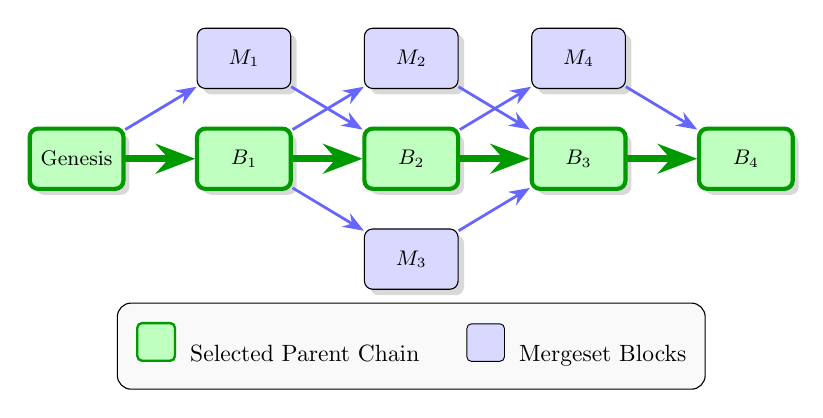
\begin{tikzpicture}[
    block/.style={rectangle, draw, fill=blue!15, minimum width=1.4cm, minimum height=0.9cm, rounded corners=3pt, font=\small, drop shadow={opacity=0.3}},
    selected/.style={rectangle, draw=green!60!black, fill=green!25, minimum width=1.4cm, minimum height=0.9cm, rounded corners=3pt, line width=1.5pt, font=\small, drop shadow={opacity=0.3}},
    arrow/.style={->, >=Stealth, thick},
    scale=0.85, transform shape
]
    % Genesis
    \node[selected] (g) at (0,0) {Genesis};
    
    % Layer 1
    \node[selected] (b1) at (2.5,0) {$B_1$};
    \node[block] (m1) at (2.5,1.5) {$M_1$};
    
    % Layer 2
    \node[selected] (b2) at (5,0) {$B_2$};
    \node[block] (m2) at (5,1.5) {$M_2$};
    \node[block] (m3) at (5,-1.5) {$M_3$};
    
    % Layer 3
    \node[selected] (b3) at (7.5,0) {$B_3$};
    \node[block] (m4) at (7.5,1.5) {$M_4$};
    
    % Layer 4
    \node[selected] (b4) at (10,0) {$B_4$};
    
    % Arrows - Selected chain (thick green)
    \draw[arrow, line width=2.5pt, green!60!black] (g) -- (b1);
    \draw[arrow, line width=2.5pt, green!60!black] (b1) -- (b2);
    \draw[arrow, line width=2.5pt, green!60!black] (b2) -- (b3);
    \draw[arrow, line width=2.5pt, green!60!black] (b3) -- (b4);
    
    % Arrows - Merge blocks (thinner, blue-gray)
    \draw[arrow, blue!60, line width=1pt] (g) -- (m1);
    \draw[arrow, blue!60, line width=1pt] (m1) -- (b2);
    \draw[arrow, blue!60, line width=1pt] (b1) -- (m2);
    \draw[arrow, blue!60, line width=1pt] (m2) -- (b3);
    \draw[arrow, blue!60, line width=1pt] (b1) -- (m3);
    \draw[arrow, blue!60, line width=1pt] (m3) -- (b3);
    \draw[arrow, blue!60, line width=1pt] (b2) -- (m4);
    \draw[arrow, blue!60, line width=1pt] (m4) -- (b4);
    
    % Legend box - positioned below the diagram
    \node[draw, rounded corners=5pt, fill=gray!5, inner sep=8pt] at (5,-2.8) {
        \begin{tabular}{@{}c@{\hspace{6pt}}l@{\hspace{20pt}}c@{\hspace{6pt}}l@{}}
            \tikz\node[rectangle, draw=green!60!black, fill=green!25, minimum width=0.5cm, minimum height=0.35cm, rounded corners=2pt, line width=1pt] {}; & Selected Parent Chain &
            \tikz\node[rectangle, draw, fill=blue!15, minimum width=0.5cm, minimum height=0.35cm, rounded corners=2pt] {}; & Mergeset Blocks
        \end{tabular}
    };
\end{tikzpicture}
\caption{GHOSTDAG PoW DAG Ledger Structure. The green blocks form the \emph{selected parent chain} (the canonical backbone determined by GHOSTDAG). Blue blocks are \emph{mergeset blocks}---parallel blocks whose transactions are merged into the ledger when a selected-chain block references them as additional parents.}
\label{fig:blockdag}
\end{figure}

Two key challenges arise in GHOSTDAG-based PoW DAG ledgers:

\textbf{Execution-Log Commitment:} How to commit each block to the global canonical order of all transactions executed up to that point, so that Layer-2 (L2) systems can trustlessly follow the exact L1 execution sequence. A straightforward approach is adding a chained commitment in each block header that hashes together the previous commitment and the Merkle root of the current block's accepted transactions: $\text{SC}_n = H(\text{SC}_{n-1} \parallel \text{ExecRoot}_n)$. While simple, a purely linear commitment implies that to prove a transaction from many blocks ago, one might need to traverse or reveal a long chain of commitments---a verification cost linear in the distance between blocks, which is prohibitive for L2 verification if the distance is large.

\textbf{Logarithmic Inclusion Proofs:} How to enable compact proofs (of size $\bigO(\log N)$) that a given transaction was included in the ledger by a certain block, without requiring a client to download or trust the entire chain history. Naive proofs of inclusion in any DAG ledger could be linear in the distance from the block to be verified. The challenge is to use a data structure that enables skip-ahead verification, reminiscent of the FlyClient approach for light clients~\cite{flyclient}.

Each of these alone solves part of the problem, but implementing them separately would mean maintaining two parallel commitment structures: one for ordering and one for efficient proofs. As noted in recent research on Merkle structures~\cite{merklebelt}, a linear hash chain is essentially a degenerate ``mountain range'' with exactly one peak that grows linearly---maximally unbalanced and far from succinct, forcing proofs to be as long as the list itself.

In this paper, we propose a unified solution that achieves both goals simultaneously by leveraging a data structure called a \textbf{Merkle Mountain Range (MMR)} as a historical accumulator of execution commitments. MMRs were first popularized by Todd for Bitcoin-like systems~\cite{todd2012mmr} as a way to commit to ever-growing data with the ability to produce logarithmic-sized proofs of membership. By replacing the linear execution-log commitment with an MMR-based execution-log accumulator, we reduce proof complexity from $\bigO(N)$ to $\bigO(\log N)$.

\subsection{From Block Ordering to Execution Ordering}

A critical insight motivating our design is the distinction between \emph{block ordering} and \emph{execution ordering}. Traditional approaches focus on committing to the order of blocks. However, what Layer-2 systems, bridges, and rollups actually need is the \textbf{execution order of transactions}---the deterministic sequence in which transactions are validated and applied to the UTXO set.

In a GHOSTDAG structure, a single block may ``merge'' transactions from multiple parallel blocks in its mergeset. The execution order is determined not by block arrival time, but by the consensus algorithm's deterministic processing of the selected parent chain. A transaction's position in the global execution order is a function of:
\begin{enumerate}
    \item Which selected-chain block processes it
    \item Its position within that block's accepted transaction list (derived from UTXO validation)
\end{enumerate}

This distinction matters because:
\begin{itemize}
    \item An L2 rollup must replay transactions in \emph{exactly} the same order to reproduce state
    \item A bridge contract verifying withdrawals needs to confirm \emph{execution position}, not just block inclusion
    \item Dispute resolution requires proving that a transaction was executed at a specific global position
\end{itemize}

Our approach makes this execution order a \textbf{first-class consensus output}: the \code{exec\_root} is computed directly from the \code{accepted\_tx\_ids} produced by the UTXO validation pipeline, not from block metadata.

\subsection{Our Contributions}

Our approach, which we call the \emph{MMR Execution-Log Commitment}, integrates with GHOSTDAG consensus as follows:
\begin{itemize}
    \item Every block contains an \code{exec\_root} computed as $\MerkleRoot(\text{accepted\_tx\_ids})$, where \code{accepted\_tx\_ids} is the deterministic output of the consensus execution pipeline (\code{calculate\_utxo\_state}). This is not a post-processing step---it is derived from the same computation that determines UTXO validity.
    \item Every block also carries an \code{elog\_root} and \code{elog\_size}, which accumulate all prior blocks' execution commitments in an append-only Merkle Mountain Range. The MMR leaf binds the block's \code{exec\_root} to its position in the selected parent chain.
    \item The combination allows any transaction's \textbf{execution position} to be proven with two linked proofs: an intra-block Merkle proof showing the transaction's index within the block's execution order, and an MMR proof showing that block's position in the global execution history.
\end{itemize}

This design effectively provides \textbf{everlasting cryptographic execution position receipts} for transactions: a light client or an L2 contract can verify that a transaction was executed at position $(j, i)$---block $j$ in the selected parent chain, transaction $i$ within that block---by checking a short proof against a recent block header's execution log root. The proof size and verification cost grow only logarithmically with the age of the transaction, rather than linearly as in a simple chained commitment scheme.

Our contributions advance the state of the art in DAG consensus verifiability:

\begin{enumerate}
    \item \textbf{New Proof Object: Execution Position Receipts} We introduce a new class of cryptographic proofs for PoW DAG ledgers: \textbf{execution position receipts} that prove a transaction was executed at position $(j, i)$ in the consensus-determined execution sequence. This differs fundamentally from inclusion proofs (which prove ``transaction is in block'') or chain membership proofs (which prove ``block is in chain''). In DAG contexts, execution order $\neq$ block order, making this a distinct and necessary proof object.
    
    \item \textbf{Consensus API Contract: Externalizing Execution as Verifiable Interface} We formalize the \textbf{Consensus API Contract}, defining \code{AcceptedTxList(B)} as the atomic output of consensus execution. This transforms GHOSTDAG from ``I executed, but you must trust me or run a full node'' to ``I executed, and here is a verifiable execution receipt.'' We prove (Theorem~\ref{thm:execution-fidelity}) that proofs verify actual execution, not just declared inclusion.
    
    \item \textbf{Consensus-Level Validation: Necessity, Not Choice} We demonstrate through a counter-example model (Attack~\ref{attack:auxiliary-divergence}) that auxiliary execution logs are insufficient for L2/bridge applications. We prove (Proposition~\ref{prop:auxiliary-insufficient}) that consensus-level validation is a security requirement, not merely a design choice. This establishes that our approach is not ``engineering optimization'' but addresses a fundamental gap in DAG verifiability.
    
    \item \textbf{Formal Security Guarantees} We provide three formal security theorems:
    \begin{itemize}
        \item \textbf{Execution-Fidelity} (Theorem~\ref{thm:execution-fidelity}): Proofs verify actual consensus execution order
        \item \textbf{Reorg-Soundness} (Theorem~\ref{thm:reorg-soundness}): Proof validity conditions under reorganization
        \item \textbf{Non-Equivocation} (Theorem~\ref{thm:non-equivocation}): Binding to unique execution history
    \end{itemize}
    These establish that execution log proofs have consensus-equivalent security (Corollary~\ref{cor:consensus-equivalent}).
    
    \item \textbf{Availability Separation Model} We formalize the separation between consensus commitments (always verifiable) and proof generation capability (availability-dependent) in Theorem~\ref{thm:availability-separation}. This enables a capability tier model where rolling MMR maintains verification guarantees while optimizing storage, addressing a key scalability challenge.
    
    \item \textbf{Unified Design: Ordering + Proofs in One Structure} Unlike previous approaches that require separate mechanisms for ordering commitment and efficient proofs, our MMR-based design provides both through a single, unified structure. The \code{exec\_root} commits to execution order; the \code{elog\_root} enables $\bigO(\log n)$ proofs. This architectural unification eliminates the need for dual commitment systems.
    
    \item \textbf{Quantitative Results} We demonstrate that verifying a transaction from 100,000 blocks ago requires only $\sim$17 hash operations ($<$1~KB proof) versus 100,000 sequential hashes in linear schemes---a 99.98\% reduction enabling on-chain verification in smart contracts.
\end{enumerate}

\subsection{Paper Organization}

The rest of this paper is organized as follows. Section~\ref{sec:background} provides background on GHOSTDAG and the need for canonical ordering and efficient proofs, including an introduction to Merkle Mountain Ranges. Section~\ref{sec:design} describes the design of the MMR execution-log accumulator in detail. Section~\ref{sec:reorg} addresses how we handle challenges like block reorganization and pruning. Section~\ref{sec:proofs} discusses the proof construction and verification. Section~\ref{sec:applications} explores important use cases and benefits. Section~\ref{sec:overhead} analyzes the overhead and performance based on experiments with Tondi, a GHOSTDAG implementation running at 10 BPS. Section~\ref{sec:comparison} compares our approach with alternative schemes. Implementation considerations are given in Section~\ref{sec:implementation}. Finally, Section~\ref{sec:conclusion} concludes with a summary and implications for future blockchain designs.

\subsection{Terminology and Notation}

For clarity, we define key terms used throughout this paper:

\begin{itemize}
    \item \textbf{Execution Position Receipt:} A cryptographic proof that a transaction was executed at position $(j, i)$---block $j$ in the selected parent chain, transaction $i$ within that block's execution sequence. This is the primary proof object our scheme produces.
    
    \item \textbf{Execution Commitment (\code{exec\_root}):} The Merkle root of the delta-executed transaction list when extending state from $\mathsf{SP}(B)$ to $B$. Commits to the execution output, not merely block contents.
    
    \item \textbf{Execution Log Accumulator (\code{elog\_root}):} The MMR root that accumulates all execution commitments in an append-only structure. Enables logarithmic proofs of execution position.
    
    \item \textbf{Consensus API Contract:} The formal interface that GHOSTDAG implementations must expose, defining \code{AcceptedTxList(B)} as the atomic output of consensus execution.
    
    \item \textbf{Selected Parent Chain:} The canonical chain determined by GHOSTDAG, formed by following selected parent links from genesis to tip.
    
    \item \textbf{Mergeset:} The set of blocks referenced by a block but not on the selected parent chain. Their transactions are merged into the execution sequence.
\end{itemize}

%==============================================================================
% SECTION 2: BACKGROUND
%==============================================================================
\section{Background and Motivation}
\label{sec:background}

\subsection{Terminology: PoW DAG Ledgers}

We study \textbf{proof-of-work DAG ledgers} (PoW DAG ledgers), often referred to as ``BlockDAG'' systems in industry. A PoW DAG ledger is a distributed ledger where blocks form a directed acyclic graph (DAG) rather than a linear chain, enabling parallel block production while maintaining a deterministic total ordering of transactions through consensus rules.

\textbf{GHOSTDAG} is a specific consensus algorithm for PoW DAG ledgers that:
\begin{itemize}
    \item Assigns each block a \emph{blue score} based on its position in the DAG
    \item Selects a canonical chain (the \emph{selected parent chain}) from the DAG
    \item Merges parallel blocks (the \emph{mergeset}) into a deterministic execution sequence
    \item Outputs a total order of accepted transactions via UTXO validation
\end{itemize}

Throughout this paper, we use \textbf{PoW DAG ledger}, \textbf{DAG ledger}, or \textbf{PoW DAG} to refer to this class of systems. The term ``BlockDAG'' appears only in this definition for clarity with industry terminology.

\subsection{Blockchain Transaction Ordering and Proofs}

In a conventional blockchain (single chain of blocks), establishing the order of transactions and providing proofs of inclusion is straightforward: all blocks form a linear sequence, and within each block a Merkle tree commits to the transactions. A client given a block header (with the Merkle root) and a transaction plus a Merkle branch can verify that transaction was included in that block. To trust that this block is part of the canonical chain, the client must also verify the chain of block hashes (or a proof-of-work difficulty sequence) from a known checkpoint up to that block.

Verifying a transaction from $N$ blocks ago thus typically requires $\bigO(\log M)$ work for the Merkle proof (where $M$ is the number of transactions in that block) plus $\bigO(N)$ work to verify the block's inclusion in the chain (unless some accumulator of block headers is used).

The DAG ledger architecture complicates transaction ordering in two ways:
\begin{enumerate}
    \item There isn't a single chain of blocks---blocks can be created concurrently and reference multiple parents. GHOSTDAG assigns a partial order to blocks and designates one parent of each block as the \emph{selected parent}.
    \item Because blocks are not strictly sequential, defining a canonical order of transactions is non-trivial. GHOSTDAG does produce a deterministic ordering of blocks, but this order must be agreed upon and consistent across all nodes.
\end{enumerate}

The motivation for having an explicit commitment to transaction ordering is largely driven by Layer-2 scalability solutions (like rollups or payment channels) and cross-chain bridges. These systems need to verify L1 events with minimal trust. Without a specialized commitment, verifying an event from an old block might require linear work in the number of blocks since then---impractical on-chain or for light clients.

\subsection{Merkle Mountain Ranges (MMR)}

Our solution employs Merkle Mountain Ranges (MMRs) as the core data structure to achieve an efficient historical commitment~\cite{herodotus}. An MMR is a type of append-only Merkle tree structure especially suited for sequentially growing datasets.

\begin{definition}[Merkle Mountain Range]
An MMR is defined over an indexed sequence of leaves (data items) numbered from $0$ onward. It can be thought of as a forest of perfect binary trees (``mountains'') whose sizes correspond to the binary decomposition of the leaf count. For $N$ leaves, if $N = \sum_{i} 2^{b_i}$ in binary, then the MMR consists of trees of sizes $2^{b_i}$.
\end{definition}

\begin{figure}[htbp]
\centering
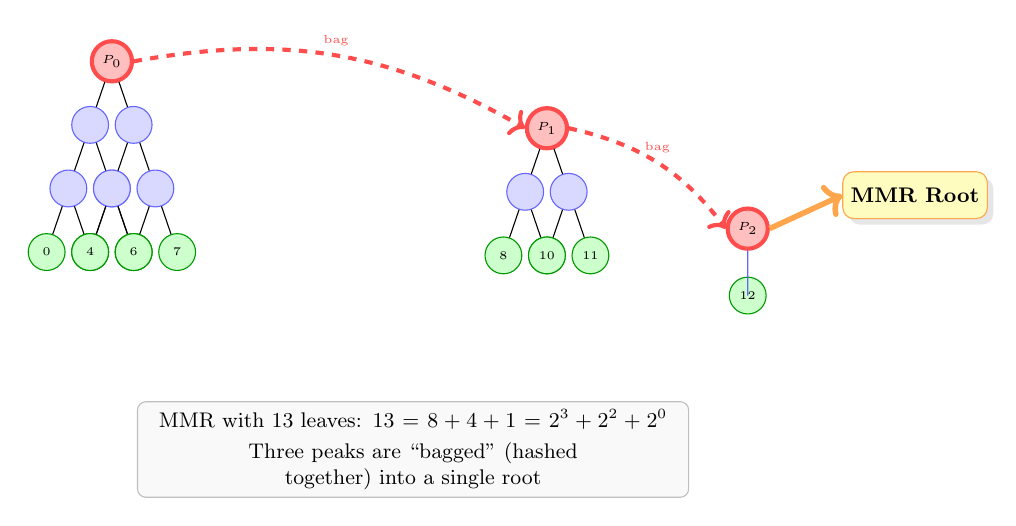
\begin{tikzpicture}[
    node/.style={circle, draw=blue!60, fill=blue!15, minimum size=0.55cm, font=\tiny, inner sep=1pt},
    leaf/.style={circle, draw=green!60!black, fill=green!20, minimum size=0.55cm, font=\tiny, inner sep=1pt},
    peak/.style={circle, draw=red!70, fill=red!25, minimum size=0.6cm, font=\tiny\bfseries, line width=1.5pt, inner sep=1pt},
    level distance=0.95cm,
    sibling distance=0.65cm,
    scale=0.85, transform shape
]
    % Mountain 1 (size 8) - positioned manually for better control
    \node[peak] (r1) at (3,3) {$P_0$}
        child {node[node] {}
            child {node[node] {}
                child {node[leaf] {0}}
                child {node[leaf] {1}}
            }
            child {node[node] {}
                child {node[leaf] {2}}
                child {node[leaf] {3}}
            }
        }
        child {node[node] {}
            child {node[node] {}
                child {node[leaf] {4}}
                child {node[leaf] {5}}
            }
            child {node[node] {}
                child {node[leaf] {6}}
                child {node[leaf] {7}}
            }
        };
    
    % Mountain 2 (size 4)
    \node[peak] (r2) at (9.5,2) {$P_1$}
        child {node[node] {}
            child {node[leaf] {8}}
            child {node[leaf] {9}}
        }
        child {node[node] {}
            child {node[leaf] {10}}
            child {node[leaf] {11}}
        };
    
    % Mountain 3 (size 1)
    \node[peak] (r3) at (12.5,0.5) {$P_2$};
    \node[leaf] at (12.5,-0.5) {12};
    \draw[blue!60] (r3) -- (12.5,-0.5);
    
    % Bagging arrows with clearer styling
    \draw[->, line width=1.5pt, dashed, red!70] (r1.east) to[bend left=20] node[above, font=\tiny, red!70] {bag} (r2.west);
    \draw[->, line width=1.5pt, dashed, red!70] (r2.east) to[bend left=20] node[above, font=\tiny, red!70] {bag} (r3.west);
    
    % Final root box
    \node[draw=orange!70, fill=yellow!25, rounded corners=4pt, font=\small\bfseries, minimum width=1.8cm, minimum height=0.7cm, drop shadow={opacity=0.2}] (root) at (15,1) {MMR Root};
    \draw[->, line width=2pt, orange!70] (r3.east) -- (root.west);
    
    % Annotation box at bottom
    \node[draw=gray!50, fill=gray!5, rounded corners=3pt, font=\small, align=center, text width=8cm] at (7.5,-2.8) {
        MMR with 13 leaves: $13 = 8 + 4 + 1 = 2^3 + 2^2 + 2^0$\\[2pt]
        Three peaks are ``bagged'' (hashed together) into a single root
    };
\end{tikzpicture}
\caption{Merkle Mountain Range structure with 13 leaves. The structure consists of three ``mountains'' (perfect binary trees) corresponding to the binary representation $13_{10} = 1101_2$. Peaks $P_0$, $P_1$, $P_2$ are hashed together (bagged) to produce the final MMR root.}
\label{fig:mmr-structure}
\end{figure}

Key properties of MMRs that make them attractive for blockchain history accumulators include:

\begin{enumerate}
    \item \textbf{Append-Only and Efficient Updates:} Adding a new leaf to an MMR takes $\bigO(\log N)$ hashing work. The MMR doesn't require a fixed tree size or re-balancing; it naturally accommodates continuous growth.
    
    \item \textbf{Succinct Proofs:} To prove that a given leaf is included in the MMR, one provides a proof consisting of the leaf's sibling nodes up through the tree and the list of peaks. The size of this proof is at most $\bigO(\log N)$ hashes.
    
    \item \textbf{Immutability and Unique Representation:} The structure of the MMR is fully determined by the number of leaves. For a given sequence of $N$ items, the MMR will always produce the same set of peak hashes and the same root.
    
    \item \textbf{Inclusion of Historical Data:} Unlike a simple moving hash (like a chain of hashes), the MMR's peaks collectively incorporate all past leaves. Even older blocks far down the ``mountain range'' are still cryptographically linked into the latest root.
\end{enumerate}

\textbf{Appending Algorithm:} When a new leaf is added to the MMR, it is appended as a new tree of size 1 (a new peak). If the previously last tree (peak) also had size 1, then the two single leaves are merged to form a tree of size 2. This might in turn merge with a next peak of size 2 to form a size 4 tree, and so on. In general, the rule is: upon adding the $(n+1)$-th leaf, look at the binary representation of $n$. Each trailing 1 in $n$ indicates a peak that will merge with the new leaf (or intermediate result of merges) to form a larger peak. This is equivalent to ``carrying'' in binary addition.

\textbf{Example:} If $n = 7$ (binary $111$, with trailing ones), there were peaks of sizes 1, 2, 4. A new leaf causes the size-1 peak and new leaf to merge (size 2), then that merges with the existing size-2 peak to form size 4, then that merges with the existing size-4 peak to form a size-8 peak. Now for $n+1 = 8$ ($1000_2$), there is just one peak of size 8. If $n = 4$ (binary $100$, already a perfect tree of size 4 with one peak), adding a leaf results in $n+1 = 5$ ($101_2$) which will have two peaks: the old size-4 peak remains and the new leaf stands alone as a size-1 peak.

\textbf{MMR vs. Linear Chain:} A linear hash chain (each block contains the hash of the previous block) is essentially an extreme case of a Merkle structure---a degenerate ``mountain range'' with exactly one peak that grows linearly. The proof that a given block was in the chain of length $N$ is of length $N$ (one would have to show each link). As noted in recent research~\cite{merklebelt}, the linear chain is maximally unbalanced and far from succinct; it forces proofs to be as long as the list itself. In contrast, an MMR is balanced and yields succinct proofs (logarithmic in $N$).

\subsection{GHOSTDAG, Selected Chain, and Consensus-Determined Transaction Sequence}
\label{sec:consensus-determined-sequence}

\textbf{GHOSTDAG PoW DAG Ledger:} A GHOSTDAG-based PoW DAG ledger is a distributed ledger where blocks reference multiple parents, forming a DAG structure. This yields high throughput (e.g., 10 blocks per second in Tondi) but requires a rule to determine a total ordering. GHOSTDAG assigns each block a \emph{blue score} and orders blocks by essentially sorting by blue score and hash. For each new block, one of its parents is labeled the \emph{selected parent} (SP)---usually the one with the highest blue score. The set of blocks not on the selected parent chain but referenced by the new block are called the block's \emph{mergeset}.

\subsubsection{Formal Model: Transaction Sequence Derivation}

We now formalize the exact sequence that our scheme commits to. This is critical: reviewers and implementers must understand \emph{precisely} which sequence is being committed.

\begin{definition}[GHOSTDAG Block Ordering]
\label{def:ghostdag-ordering}
For a block $B$ on the selected parent chain, define:
\begin{itemize}
    \item $\mathsf{SP}(B)$: The selected parent of $B$
    \item $\mathsf{Mergeset}(B)$: The set of blocks referenced by $B$ but not on the selected parent chain
    \item $\mathsf{MergesetOrder}(B)$: A deterministic total ordering of $\mathsf{Mergeset}(B)$, typically by $(blue\_score, block\_hash)$ lexicographically
\end{itemize}
\end{definition}

\begin{definition}[Intra-Block Transaction Ordering]
\label{def:intra-block-ordering}
For each block $M$, define $\mathsf{TxOrder}(M)$ as the sequence of transactions in $M$'s body, ordered by their position in the block's transaction list (as serialized in the block). This ordering is \textbf{miner-chosen} but \textbf{consensus-fixed} once the block is created.
\end{definition}

\begin{definition}[Conflict Resolution Rule]
\label{def:conflict-resolution}
When processing transactions, if transaction $tx_a$ and $tx_b$ conflict (e.g., double-spend the same UTXO):
\begin{enumerate}
    \item If they appear in different blocks: the transaction in the \emph{earlier} block (per $\mathsf{MergesetOrder}$) wins
    \item If they appear in the same block: the transaction with \emph{lower index} (per $\mathsf{TxOrder}$) wins
\end{enumerate}
The losing transaction is \textbf{rejected} and does not appear in $\mathsf{AcceptedTxList}$.
\end{definition}

\begin{definition}[Canonical Execution Sequence]
\label{def:canonical-execution-sequence}
For a block $B$ on the selected parent chain, the \emph{canonical execution sequence} $\mathsf{TxList}(B)$ is constructed as follows:

\begin{enumerate}
    \item Let $\mathsf{BlockSeq}(B) = [\mathsf{SP}(B)] \oplus \mathsf{MergesetOrder}(B) \oplus [B]$
    \item For each block $M \in \mathsf{BlockSeq}(B)$ in order:
    \begin{enumerate}
        \item For each $tx \in \mathsf{TxOrder}(M)$ in order:
        \begin{enumerate}
            \item If $tx$ is valid against current UTXO state and not conflicting with already-accepted transactions: accept $tx$, append $tx.id$ to $\mathsf{TxList}(B)$, update UTXO state
            \item Otherwise: reject $tx$ (do not append)
        \end{enumerate}
    \end{enumerate}
\end{enumerate}

This produces a \textbf{deterministic, ordered list} of accepted transaction IDs.
\end{definition}

\begin{proposition}[Consensus Uniqueness]
\label{prop:consensus-uniqueness}
For any block $B$ and any two honest nodes $N_1, N_2$:
\[
\mathsf{TxList}_{N_1}(B) = \mathsf{TxList}_{N_2}(B)
\]
provided both nodes have the same view of the DAG up to $B$.
\end{proposition}

\textbf{Proof Sketch:} The sequence depends only on: (1) the DAG structure (which blocks exist and their parent relationships), (2) the GHOSTDAG blue score assignments (deterministic from DAG), (3) the block body contents (transactions and their ordering). All three are consensus-determined and identical across honest nodes. \qed

\textbf{Key Insight:} The miner of block $B$ controls $\mathsf{TxOrder}(B)$ (the ordering of $B$'s own transactions), but \emph{not} the ordering of mergeset blocks or the conflict resolution outcome. Thus, while miners have some influence over ordering, the \emph{overall sequence across the selected chain} is consensus-determined, not miner-arbitrary.

\begin{definition}[Execution Root]
\label{def:exec-root}
For a block $B$:
\[
\mathsf{ExecRoot}(B) = \mathsf{MerkleRoot}(\mathsf{AcceptedTxList}(B))
\]
where $\mathsf{MerkleRoot}$ computes a standard binary Merkle tree over the ordered list of transaction IDs, using BLAKE3-256 for all internal node hashing. This ensures consistency with the MMR hash function and prevents cross-context collisions.
\end{definition}

This formalization ensures that $\mathsf{ExecRoot}(B)$ commits to a \textbf{precisely defined, consensus-unique sequence}---not an implementation-dependent artifact.

\subsubsection{Consensus API Contract}
\label{sec:consensus-api-contract}

For our execution log scheme to be implementable, GHOSTDAG implementations \rfc{must} expose a specific interface. We formalize this as a \textbf{Consensus API Contract}:

\begin{definition}[Consensus API Contract]
\label{def:consensus-api-contract}
A GHOSTDAG implementation supporting the execution log \rfc{must} provide the following deterministic function:
\begin{equation}
\texttt{AcceptedTxList}(B) \rightarrow [tx_1, tx_2, \ldots, tx_k]
\end{equation}
where the output is the \textbf{ordered list} of transaction IDs accepted when validating block $B$. This function \rfc{must} satisfy:
\begin{enumerate}
    \item \textbf{Determinism:} For any block $B$ and parent state $S$, all honest nodes produce identical output
    \item \textbf{Atomicity:} The list is produced atomically with UTXO state transition
    \item \textbf{Totality:} Every accepted transaction appears exactly once in the list
    \item \textbf{Conflict Resolution:} Double-spends are resolved before output; only winners appear
\end{enumerate}
\end{definition}

\textbf{Interface Binding:} In practice, this maps directly to existing GHOSTDAG implementations. For example, in a typical implementation:
\begin{lstlisting}[language=Python, caption={Consensus API Contract binding}, basicstyle=\scriptsize\ttfamily]
def calculate_utxo_state(block, parent_state):
    ctx = UTXOContext(parent_state)
    # Process selected parent, mergeset, and block's own txs
    for tx in ordered_transactions(block):
        if ctx.validate_and_apply(tx):
            ctx.accepted_tx_ids.append(tx.id)
    return ctx  # ctx.accepted_tx_ids is AcceptedTxList(B)
\end{lstlisting}

\textbf{Reorg Semantics:} When a reorganization occurs (selected chain changes), the \code{AcceptedTxList} for affected blocks \rfc{must} be recomputed. The execution log tracks the \emph{current} selected chain view; historical proofs become invalid if the chain reorganizes past their anchor point. We formalize this in Section~\ref{sec:reorg-checkpoint}.

\begin{figure}[htbp]
\centering
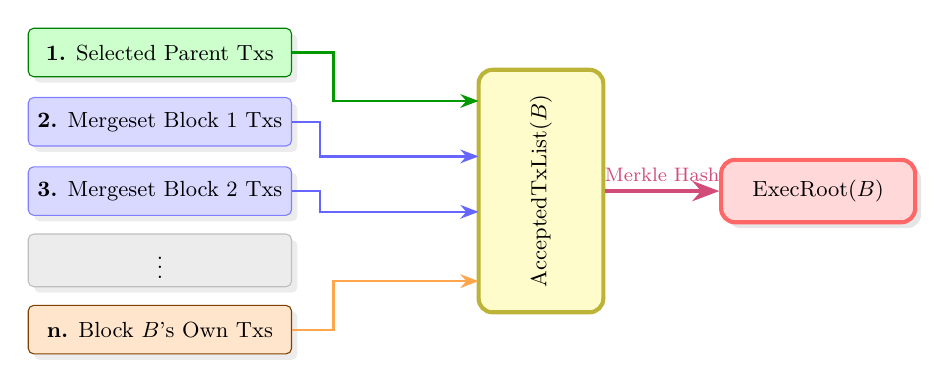
\begin{tikzpicture}[
    box/.style={rectangle, draw, rounded corners=2pt, minimum width=3.8cm, minimum height=0.7cm, font=\small, drop shadow={opacity=0.15}},
    arrow/.style={->, >=Stealth, thick},
    scale=0.88, transform shape
]
    % Input boxes with numbered order
    \node[box, fill=green!20, draw=green!50!black] (sp) at (0,4) {\textbf{1.} Selected Parent Txs};
    \node[box, fill=blue!15, draw=blue!50] (m1) at (0,3) {\textbf{2.} Mergeset Block 1 Txs};
    \node[box, fill=blue!15, draw=blue!50] (m2) at (0,2) {\textbf{3.} Mergeset Block 2 Txs};
    \node[box, fill=gray!15, draw=gray!50] (dots) at (0,1) {$\vdots$};
    \node[box, fill=orange!20, draw=orange!50!black] (own) at (0,0) {\textbf{n.} Block $B$'s Own Txs};
    
    % TxList container
    \node[draw=yellow!70!black, rounded corners=5pt, fill=yellow!20, minimum width=1.8cm, minimum height=3.5cm, line width=1.5pt] (txlist) at (5.5,2) {};
    \node[font=\small\bfseries, rotate=90] at (5.5,2) {$\AcceptedTxList(B)$};
    
    % Arrows to TxList
    \draw[arrow, green!60!black] (sp.east) -- ++(0.6,0) |- (4.6,3.3);
    \draw[arrow, blue!60] (m1.east) -- ++(0.4,0) |- (4.6,2.5);
    \draw[arrow, blue!60] (m2.east) -- ++(0.4,0) |- (4.6,1.7);
    \draw[arrow, orange!70] (own.east) -- ++(0.6,0) |- (4.6,0.7);
    
    % OrderRoot
    \node[draw=red!60, rounded corners=5pt, fill=red!15, minimum width=2.8cm, minimum height=0.9cm, line width=1.5pt, font=\small\bfseries, drop shadow={opacity=0.2}] (orderroot) at (9.5,2) {$\ExecRoot(B)$};
    
    % Arrow with label
    \draw[arrow, line width=1.5pt, purple!70] (txlist.east) -- node[above, font=\footnotesize, text=purple!70] {Merkle Hash} (orderroot.west);
\end{tikzpicture}
\caption{Construction of the canonical transaction list ($\AcceptedTxList$) and $\ExecRoot$ for block $B$. Transactions are ordered deterministically: selected parent first, then mergeset blocks in consensus order, finally block $B$'s own transactions.}
\label{fig:txlist-construction}
\end{figure}

A GHOSTDAG node implementation computes, for each block $B$, the set of \emph{accepted transaction IDs}---essentially the union of the transactions in the block's selected parent and those in the block's remaining mergeset (excluding conflicts), in a deterministic order. By walking through the DAG following the selected chain and at each block outputting its accepted transaction list, one obtains a single global sequence of transactions. This global sequence is what an L2 system would interpret as the history of L1 transactions.

\textbf{Detailed Example:} Consider a simple DAG scenario for illustration. Suppose block $B_1$ is the genesis, and two blocks $B_2$ and $B_3$ are mined concurrently on $B_1$. Then a block $B_4$ comes selecting $B_2$ as its parent, and another $B_5$ selecting $B_3$, and finally $B_6$ selecting $B_4$ and also referencing $B_5$:
\begin{center}
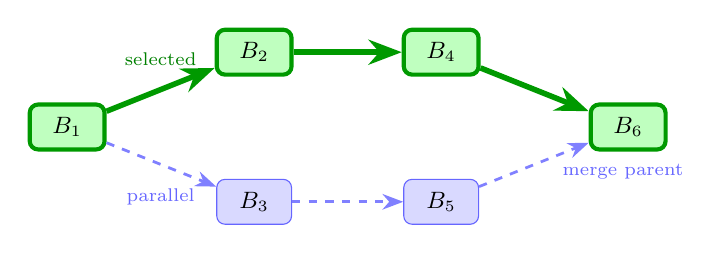
\begin{tikzpicture}[
    block/.style={rectangle, draw=blue!60, fill=blue!15, minimum width=1cm, minimum height=0.6cm, font=\small, rounded corners=3pt},
    selected/.style={rectangle, draw=green!60!black, fill=green!25, minimum width=1cm, minimum height=0.6cm, font=\small, line width=1.5pt, rounded corners=3pt},
    selarrow/.style={->, >=Stealth, line width=2pt, green!60!black},
    mergearrow/.style={->, >=Stealth, line width=1pt, blue!50, dashed},
    scale=0.95, transform shape
]
    % Nodes
    \node[selected] (b1) at (0,0) {$B_1$};
    \node[selected] (b2) at (2.5,1) {$B_2$};
    \node[block] (b3) at (2.5,-1) {$B_3$};
    \node[selected] (b4) at (5,1) {$B_4$};
    \node[block] (b5) at (5,-1) {$B_5$};
    \node[selected] (b6) at (7.5,0) {$B_6$};
    
    % Selected parent chain arrows (solid, thick, green)
    \draw[selarrow] (b1) -- (b2);
    \draw[selarrow] (b2) -- (b4);
    \draw[selarrow] (b4) -- (b6);
    
    % Other parent arrows (dashed, thinner, blue)
    \draw[mergearrow] (b1) -- (b3);
    \draw[mergearrow] (b3) -- (b5);
    \draw[mergearrow] (b5) -- (b6);
    
    % Labels
    \node[font=\scriptsize, text=green!50!black, above] at (1.25,0.7) {selected};
    \node[font=\scriptsize, text=blue!60, below] at (1.25,-0.7) {parallel};
    \node[font=\scriptsize, text=blue!60, right] at (6.5,-0.6) {merge parent};
\end{tikzpicture}
\end{center}

Here the selected parent chain is: $B_1 \to B_2 \to B_4 \to B_6$ (green blocks). The canonical transaction sequence up to $B_6$ would then be:
\begin{enumerate}[noitemsep]
    \item $\AcceptedTxList(B_1)$: all transactions from genesis
    \item $\AcceptedTxList(B_2)$: transactions from $B_2$
    \item Transactions from $B_3$ not already included (merged when $B_4$ or $B_6$ processes its mergeset)
    \item $\AcceptedTxList(B_4)$: transactions from $B_4$
    \item Transactions from $B_5$ not already included (merged when $B_6$ is processed)
    \item $\AcceptedTxList(B_6)$: transactions from $B_6$
\end{enumerate}
This results in one total order of all accepted transactions up to block $B_6$. If two transactions conflict (double-spend), GHOSTDAG consensus ensures only one will be accepted---generally the one appearing in the earlier position in the canonical order.

A linear sequencing mechanism would maintain a running hash chain: $SC_n = H(SC_{n-1} \parallel \ExecRoot(B_n))$. While this achieves commitment to the sequence, it inherits a major limitation: verifying that a given old block's transactions are in the chain up to some later point requires iterating through each block's hash link in between (linear complexity). Our approach replaces this linear chain of commitments with the MMR accumulator, which breaks the sequential dependency and allows skip-ahead verification.

%==============================================================================
% SECTION 3: DESIGN
%==============================================================================
\section{MMR Execution-Log Commitment Design}
\label{sec:design}

In this section, we present the detailed design of the MMR-based execution-log accumulator. We describe the modifications to the GHOSTDAG block header, define how the MMR is computed and updated with each new block, and specify the consensus rules for validation.

\subsection{Block Header Modifications}

We extend the GHOSTDAG block header with two new fields and modify one existing field:

\begin{longtable}{@{}llp{7cm}@{}}
\caption{Block Header Field Modifications}
\label{tab:header-fields} \\
\toprule
\textbf{Field} & \textbf{Size} & \textbf{Description} \\
\midrule
\endfirsthead
\multicolumn{3}{c}{{\bfseries \tablename\ \thetable{} -- continued from previous page}} \\
\toprule
\textbf{Field} & \textbf{Size} & \textbf{Description} \\
\midrule
\endhead
\midrule \multicolumn{3}{r}{{Continued on next page}} \\
\endfoot
\bottomrule
\endlastfoot
\code{exec\_root} & 32 bytes & Merkle root of accepted transaction IDs for this block, representing the set of transactions (in canonical order) confirmed by this block's addition to the ledger \\
\code{elog\_root} & 32 bytes & MMR root hash after inserting this block's leaf, serving as a cryptographic commitment to the entire history of transaction order \\
\code{elog\_size} & 8 bytes & Total number of leaves in the MMR after adding this block \\
\midrule
\multicolumn{3}{l}{\textit{Removed field:}} \\
\code{accepted\_id\_merkle\_root} & 32 bytes & (Replaced by \code{exec\_root}) \\
\midrule
\textbf{Net Change} & \textbf{+40 bytes} & ($2 \times 32 + 8 - 32 = 40$ bytes per header) \\
\end{longtable}

At 10 blocks/sec, the net increase is $\sim$34.6 MB per day, which is negligible overhead for network transmission (roughly 0.08\% of typical block data throughput).

\subsection{Consensus Impact Statement}
\label{sec:consensus-impact}

We explicitly characterize the consensus-level changes required by this proposal:

\begin{longtable}{@{}p{3.5cm}p{2cm}p{7cm}@{}}
\caption{Consensus Impact Summary}
\label{tab:consensus-impact-summary} \\
\small
\toprule
\textbf{Aspect} & \textbf{Impact} & \textbf{Details} \\
\midrule
\endfirsthead
\multicolumn{3}{c}{{\bfseries \tablename\ \thetable{} -- continued from previous page}} \\
\toprule
\textbf{Aspect} & \textbf{Impact} & \textbf{Details} \\
\midrule
\endhead
\midrule \multicolumn{3}{r}{{Continued on next page}} \\
\endfoot
\bottomrule
\endlastfoot
Block hash computation & \textbf{Changed} & Block hash now includes \code{exec\_root}, \code{elog\_root}, \code{elog\_size} \\
Validation rules & \textbf{Extended} & Nodes must validate new fields (see below) \\
PoW security & \textbf{Unchanged} & PoW target and difficulty adjustment unaffected \\
Fork choice rule & \textbf{Unchanged} & GHOSTDAG blue score / selected parent rules unchanged \\
Activation & \textbf{Hard fork} & Requires coordinated upgrade at designated height \\
\end{longtable}

\subsubsection{New Validation Rules}

Each validating node \rfc{must} perform the following checks when receiving a new block $B$:

\begin{enumerate}
    \item \textbf{ExecRoot Validation:}
    \begin{enumerate}
        \item Execute \code{calculate\_utxo\_state(B)} to obtain \code{ctx.accepted\_tx\_ids}
        \item Compute $\mathsf{expected\_exec\_root} = \mathsf{MerkleRoot}(\text{ctx.accepted\_tx\_ids})$
        \item \rfc{Reject} block if $B.\text{exec\_root} \neq \mathsf{expected\_exec\_root}$
    \end{enumerate}
    
    \item \textbf{ElogRoot Validation:}
    \begin{enumerate}
        \item Retrieve MMR state from $B$'s selected parent: $\mathsf{mmr\_state} = \mathsf{GetMmrState}(\mathsf{SP}(B))$
        \item Compute leaf: $L = H_{\text{leaf}}(\mathsf{DOMAIN\_LEAF} \| \mathsf{hash}(\mathsf{SP}(B)) \| B.\text{exec\_root})$
        \item Append leaf: $(\mathsf{new\_state}, \mathsf{expected\_root}) = \mathsf{mmr\_state.append}(L)$
        \item \rfc{Reject} block if $B.\text{elog\_root} \neq \mathsf{expected\_root}$
        \item \rfc{Reject} block if $B.\text{elog\_size} \neq \mathsf{new\_state.size}$
    \end{enumerate}
\end{enumerate}

\subsubsection{Impact on Block Hash}

The block header hash (used for PoW and block identification) \rfc{must} include the new fields. This ensures:
\begin{itemize}
    \item A miner cannot change execution log fields without re-mining
    \item The execution log commitment is protected by PoW security
    \item Block identity is bound to execution history commitment
\end{itemize}

\subsubsection{Reorg Handling}

When the selected parent chain changes (reorganization):
\begin{enumerate}
    \item Identify the common ancestor $C$ of old and new chains
    \item For each block from $C$ to new tip: recompute MMR state (peaks and size)
    \item \textbf{Invariant:} MMR state is stored per-block, not just at virtual tip
\end{enumerate}

This is $\bigO(k)$ where $k$ is the reorg depth, typically small.

\subsubsection{Activation and Upgrade Path}

\begin{itemize}
    \item \textbf{Activation height:} A predetermined block height/score at which validation rules become enforced
    \item \textbf{Genesis initialization:} The genesis block has $\mathsf{elog\_root} = \emptyset$ (empty MMR), $\mathsf{elog\_size} = 0$
    \item \textbf{Backward compatibility:} Pre-activation blocks do not have execution log fields; post-activation nodes must not validate these fields for old blocks
    \item \textbf{Upgrade requirement:} All validating nodes must upgrade before activation height (hard fork)
\end{itemize}

\subsection{Canonical Execution Order and ExecRoot Computation}

\begin{definition}[Canonical Transaction List]
For each block $B$, we define an ordered list of transaction IDs, denoted $\AcceptedTxList(B)$, which is the sequence of all accepted transactions \textbf{as determined by the consensus execution pipeline}. Critically, this is not a separate computation---it is the direct output of \code{calculate\_utxo\_state()}, specifically the \code{accepted\_tx\_ids} field of the \code{UtxoProcessingContext}.
\end{definition}

\textbf{Important Disambiguation:} $\AcceptedTxList(B)$ represents the \textbf{delta-executed} transaction IDs when extending the ledger from state at $\mathsf{SP}(B)$ to state at $B$. This includes:
\begin{itemize}
    \item Transactions from the selected parent $P_{\text{sel}}$ that were not previously executed
    \item Transactions from mergeset blocks (processed in deterministic order)
    \item Transactions from block $B$'s own body
\end{itemize}
$\AcceptedTxList(B)$ is \emph{not} limited to transactions physically contained in block $B$'s body. A transaction that appears in a mergeset block and is executed when processing block $B$ belongs to $\AcceptedTxList(B)$, and proofs for that transaction reference block $B$ as the execution block, even though the transaction's physical location is in a different block.

The \code{calculate\_utxo\_state()} function processes:
\begin{enumerate}
    \item The coinbase transaction of the selected parent $P_{\text{sel}}$ (position 0)
    \item Other transactions from $P_{\text{sel}}$, in their original block order, validated against UTXO
    \item Transactions from mergeset blocks, ordered by \code{consensus\_ordered\_mergeset\_without\_selected\_parent}, each block's transactions in original order
    \item Each transaction is validated; conflicts are deterministically resolved (first valid wins)
\end{enumerate}

\textbf{Key Design Principle:} We do \emph{not} recompute or reorder transactions for the commitment. We directly use the \code{accepted\_tx\_ids} output from consensus:

\begin{equation}
\AcceptedTxList(B) := \text{ctx.accepted\_tx\_ids} \quad \text{(from \code{UtxoProcessingContext})}
\end{equation}

\begin{equation}
\ExecRoot(B) := \MerkleRoot(\AcceptedTxList(B))
\end{equation}

\textbf{Critical Semantics:} The \code{exec\_root} commits to the \textbf{ordered list of transactions accepted when extending state from $\mathsf{SP}(B)$ to $B$} (including mergeset-derived transactions), not merely transactions included in $B$'s body. This is the \emph{delta-executed} transaction list produced during consensus processing of block $B$, representing the execution that occurred while processing this block.

\textbf{Consensus Integration:} The \code{exec\_root} is validated as part of block acceptance. If the miner's claimed \code{exec\_root} does not match $\MerkleRoot(\text{accepted\_tx\_ids})$, the block is rejected with \code{BadExecRoot}. This makes the execution order commitment a \emph{consensus-level} requirement, not an auxiliary log.

\begin{lstlisting}[language=Python,caption=ExecRoot Computation (Pseudocode)]
def compute_exec_root(ctx):
    # ctx.accepted_tx_ids is the deterministic output
    # of calculate_utxo_state() - we use it directly
    return merkle_root(ctx.accepted_tx_ids)
\end{lstlisting}

\textbf{Why This Matters:} By deriving \code{exec\_root} from the same computation that determines UTXO validity, we ensure that:
\begin{itemize}
    \item A wrong \code{exec\_root} = consensus violation = block rejected
    \item The commitment reflects \emph{actual execution}, not just declared block contents
    \item L2 systems can trust that the order matches what would be executed
\end{itemize}

\subsection{MMR Leaf and Internal Hashing Scheme}

For each block $B$ that lies on the selected parent chain, we create an MMR leaf node that binds the block's \textbf{execution output} to its \textbf{chain position}:

\begin{equation}
L(B) = \Hleaf(\text{DOMAIN\_LEAF} \parallel h_{P_{\text{sel}}(B)} \parallel \ExecRoot(B))
\end{equation}
where:
\begin{itemize}
    \item $\text{DOMAIN\_LEAF}$ is a fixed domain separation prefix (\code{``ELOG\_LEAF\_V1''})
    \item $h_{P_{\text{sel}}(B)}$ is the hash of $B$'s selected parent block header
    \item $\ExecRoot(B)$ is the Merkle root of accepted transactions (execution order commitment)
\end{itemize}

\textbf{Design Rationale (Three Critical Properties):}
\begin{enumerate}
    \item \textbf{Avoids Self-Hash Circular Dependency:} We do \emph{not} include the block's own hash $h_B$ in the leaf. This is essential because $h_B = H(\text{header})$ and the header contains \code{elog\_root}, which depends on the leaf. Including $h_B$ would create an unsolvable circular dependency.
    
    \item \textbf{Binds MMR to Execution Order:} By including $\ExecRoot(B)$, the MMR leaf commits to the \emph{execution output} of block $B$, not just its existence. A change in execution order (different \code{accepted\_tx\_ids}) changes the leaf hash, which changes the MMR root.
    
    \item \textbf{Enables Proof-Execution Alignment:} The proof verifier can reconstruct the leaf from $(h_{P_{\text{sel}}}, \ExecRoot)$---both of which are available from block headers. This allows verification without access to block bodies.
    
    \item \textbf{Prevents Leaf Replay/Relocation Attacks:} The \code{parent\_hash} binds the leaf to the specific selected-parent state from which execution proceeded. This prevents an attacker from taking a valid \code{exec\_root} from one chain position and replaying it at a different position (e.g., moving a leaf from index $j$ to index $j'$). Without \code{parent\_hash}, the same \code{exec\_root} could appear at multiple positions, breaking the one-to-one mapping between leaf index and execution position.
\end{enumerate}

\textbf{Critical Constraint:} The MMR append order \rfc{MUST} follow the selected-parent-chain order. Specifically, if blocks $B_1, B_2, \ldots, B_n$ form the selected parent chain (in order), then MMR leaves are appended in that exact sequence: $L(B_1), L(B_2), \ldots, L(B_n)$. The leaf index $j$ corresponds to the block's position in the selected chain, not its position in any other ordering (e.g., DAA score ordering or blue score ordering). This ensures that the hierarchical position $(j, i)$ in proofs unambiguously refers to "block $j$ in the selected parent chain, transaction $i$ within that block's execution."

\textbf{Why Not Include Mergeset Hash or Blue Score?}
\begin{itemize}
    \item \textbf{Mergeset hash:} The mergeset composition is already reflected in $\ExecRoot(B)$ through the deterministic mergeset ordering and conflict resolution. Including a separate mergeset hash would be redundant and increase proof size without adding security.
    \item \textbf{Blue score:} The selected parent hash $h_{P_{\text{sel}}}$ already uniquely identifies the chain position. Blue score is a derived property from the DAG structure; binding to the parent hash is more direct and avoids potential ambiguity if blue score calculation changes.
    \item \textbf{Why parent\_hash is sufficient:} Even if multiple blocks share the same selected parent (in different forks), the pair $(h_{P_{\text{sel}}}, \ExecRoot)$ is unique because:
    \begin{enumerate}
        \item Different execution contexts (different mergesets or UTXO states) produce different $\ExecRoot$ values
        \item Even if $\ExecRoot$ were identical, the blocks would have different header hashes (due to different PoW, timestamps, etc.), causing the chains to diverge
        \item The MMR append order follows the selected chain, so leaf index $j$ uniquely identifies position
    \end{enumerate}
\end{itemize}

\textbf{Why Not Include \code{tx\_count} or \code{daa\_score}?}
\begin{itemize}
    \item \code{tx\_count}: Already implicit in $\ExecRoot$ (the Merkle root structure encodes tree shape)
    \item \code{daa\_score}: Redundant---$h_{P_{\text{sel}}}$ uniquely identifies chain position
    \item Minimizing leaf contents simplifies proofs without losing security
\end{itemize}

\textbf{Leaf Uniqueness:} The pair $(h_{P_{\text{sel}}(B)}, \ExecRoot(B))$ uniquely identifies a block's execution commitment. Two blocks with the same selected parent but different accepted transactions produce different leaves. Two blocks with different parents produce different leaves regardless of transactions. This binding prevents leaf relocation attacks: an attacker cannot reuse a valid \code{exec\_root} at a different MMR position without also changing the parent hash, which would require re-mining the block and all descendants.

\subsubsection{Hash Function Specification}
\label{sec:hash-spec}

For reproducibility, we specify all hash computations precisely:

\begin{longtable}{@{}p{2cm}p{4cm}p{6.5cm}@{}}
\caption{Domain-Separated Hash Specifications}
\label{tab:hash-spec} \\
\small
\toprule
\textbf{Context} & \textbf{Domain Prefix} & \textbf{Input Format} \\
\midrule
\endfirsthead
\multicolumn{3}{c}{{\bfseries \tablename\ \thetable{} -- continued from previous page}} \\
\toprule
\textbf{Context} & \textbf{Domain Prefix} & \textbf{Input Format} \\
\midrule
\endhead
\midrule \multicolumn{3}{r}{{Continued on next page}} \\
\endfoot
\bottomrule
\endlastfoot
Leaf & \code{ELOG\_LEAF\_V1} & $\mathsf{prefix} \| h_{\text{parent}} \| \mathsf{exec\_root}$ \\
Internal Node & \code{ELOG\_NODE\_V1} & $\mathsf{prefix} \| h_{\text{left}} \| h_{\text{right}}$ \\
Peak Bagging & \code{ELOG\_BAG\_V1} & $\mathsf{prefix} \| h_{\text{acc}} \| h_{\text{peak}}$ \\
MMR Root & \code{ELOG\_ROOT\_V1} & $\mathsf{prefix} \| h_{\text{bag}} \| \mathsf{size\_le64}$ \\
\midrule
ExecRoot & (standard Merkle) & Binary Merkle tree over $[\mathsf{tx\_id}_1, \ldots, \mathsf{tx\_id}_k]$ \\
\end{longtable}

\textbf{Encoding Rules:}
\begin{itemize}
    \item \textbf{Hash function:} BLAKE3-256 (256-bit output). \rfc{MUST} be BLAKE3-256; no alternative hash functions allowed in consensus.
    \item \textbf{Domain prefixes:} ASCII-encoded strings, null-terminated (single `\textbackslash x00` byte). \textbf{No fixed-length padding required}. The exact byte sequence \rfc{MUST} match the specified strings exactly.
    \item \textbf{Hash values:} 32 bytes, big-endian
    \item \textbf{Size encoding:} 8 bytes, little-endian unsigned 64-bit integer
    \item \textbf{Concatenation:} Direct byte concatenation, no length prefixes
\end{itemize}

\textbf{Domain Separation Constants (Consensus-Mandated):}
\begin{itemize}
    \item \code{ELOG\_LEAF\_V1} = ASCII bytes \code{"ELOG\_LEAF\_V1"} + `\textbackslash x00` (null terminator)
    \item \code{ELOG\_NODE\_V1} = ASCII bytes \code{"ELOG\_NODE\_V1"} + `\textbackslash x00` (null terminator)
    \item \code{ELOG\_BAG\_V1} = ASCII bytes \code{"ELOG\_BAG\_V1"} + `\textbackslash x00` (null terminator)
    \item \code{ELOG\_ROOT\_V1} = ASCII bytes \code{"ELOG\_ROOT\_V1"} + `\textbackslash x00` (null terminator)
\end{itemize}

\textbf{Exact Byte Sequences (for reproducibility):}
\begin{itemize}
    \item \code{ELOG\_LEAF\_V1}: \code{0x45 0x4C 0x4F 0x47 0x5F 0x4C 0x45 0x41 0x46 0x5F 0x56 0x31 0x00}
    \item \code{ELOG\_NODE\_V1}: \code{0x45 0x4C 0x4F 0x47 0x5F 0x4E 0x4F 0x44 0x45 0x5F 0x56 0x31 0x00}
    \item \code{ELOG\_BAG\_V1}: \code{0x45 0x4C 0x4F 0x47 0x5F 0x42 0x41 0x47 0x5F 0x56 0x31 0x00}
    \item \code{ELOG\_ROOT\_V1}: \code{0x45 0x4C 0x4F 0x47 0x5F 0x52 0x4F 0x4F 0x54 0x5F 0x56 0x31 0x00}
\end{itemize}

\textbf{Versioning:} Future protocol upgrades \rfc{SHOULD} increment the version suffix (e.g., \code{ELOG\_LEAF\_V2}) to maintain backward compatibility while enabling new hash schemes.

\textbf{Example (Leaf Hash):}
\begin{lstlisting}[language=Python, caption={Leaf hash computation example}]
def compute_leaf(parent_hash: bytes, exec_root: bytes) -> bytes:
    domain = b"ELOG_LEAF_V1\x00"  # ASCII string + null terminator
    preimage = domain + parent_hash + exec_root
    return blake3(preimage)  # BLAKE3-256, returns 32 bytes
\end{lstlisting}

This specification ensures that independent implementations produce identical results, enabling cross-client verification.

\begin{figure}[htbp]
\centering
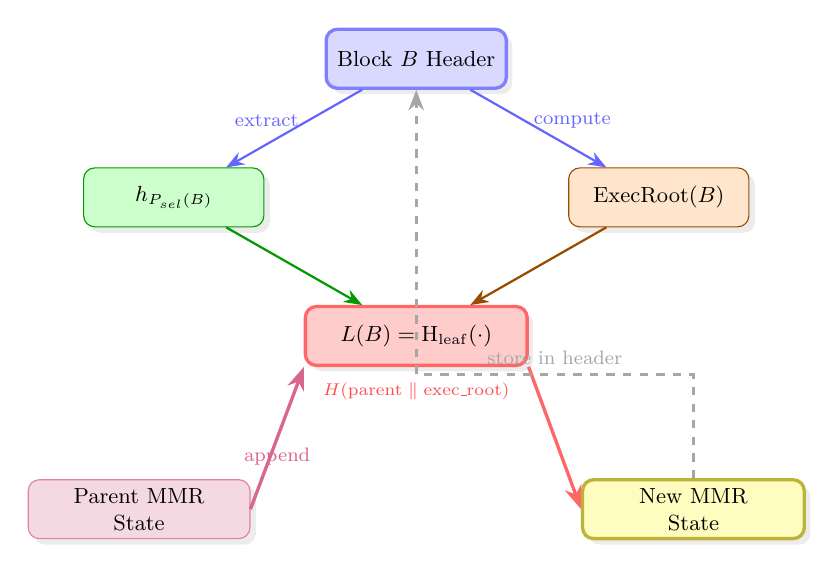
\begin{tikzpicture}[
    box/.style={rectangle, draw, rounded corners=4pt, minimum width=2.6cm, minimum height=0.85cm, font=\small, drop shadow={opacity=0.15}},
    arrow/.style={->, >=Stealth, thick},
    scale=0.88, transform shape
]
    % Block B Header (top)
    \node[box, fill=blue!15, draw=blue!50, line width=1.2pt] (header) at (0,3.5) {Block $B$ Header};
    
    % Parent Hash (left)
    \node[box, fill=green!20, draw=green!60!black] (parent) at (-3.5,1.5) {$h_{P_{sel}(B)}$};
    
    % OrderRoot (right)
    \node[box, fill=orange!20, draw=orange!60!black] (order) at (3.5,1.5) {$\ExecRoot(B)$};
    
    % Leaf hash (center)
    \node[box, fill=red!20, draw=red!60, line width=1.2pt, minimum width=3.2cm] (leaf) at (0,-0.5) {$L(B) = \Hleaf(\cdot)$};
    
    % MMR State boxes
    \node[box, fill=purple!15, draw=purple!50, minimum width=3.2cm, align=center] (mmrstate) at (-4,-3) {Parent MMR\\State};
    
    \node[box, fill=yellow!25, draw=yellow!70!black, minimum width=3.2cm, align=center, line width=1.2pt] (newmmr) at (4,-3) {New MMR\\State};
    
    % Arrows with labels
    \draw[arrow, blue!60] (header) -- node[left, font=\footnotesize, pos=0.4] {extract} (parent);
    \draw[arrow, blue!60] (header) -- node[right, font=\footnotesize, pos=0.4] {compute} (order);
    \draw[arrow, green!60!black] (parent) -- (leaf);
    \draw[arrow, orange!60!black] (order) -- (leaf);
    \draw[arrow, purple!60, line width=1.2pt] (mmrstate.east) -- node[below, font=\footnotesize, text=purple!60] {append} (leaf.south west);
    \draw[arrow, red!60, line width=1.2pt] (leaf.south east) -- (newmmr.west);
    
    % Feedback loop (dashed)
    \draw[arrow, dashed, gray!70, line width=1pt] (newmmr.north) -- ++(0,1.5) -| node[pos=0.25, above, font=\footnotesize, text=gray!70] {store in header} (header.south);
    
    % Hash symbol at leaf
    \node[font=\scriptsize, text=red!70] at (0,-1.3) {$H(\text{parent} \parallel \text{exec\_root})$};
\end{tikzpicture}
\caption{MMR leaf computation and state update flow. The leaf is computed from parent hash and $\ExecRoot$, then appended to the parent's MMR state to produce the new MMR root stored in the block header.}
\label{fig:mmr-computation}
\end{figure}

\textbf{MMR Structure Maintenance:} The MMR is maintained as follows. Let $S(n)$ denote the state of the MMR after processing $n$ leaves. The initial state $S(0)$ has an empty peaks list and size 0:
\begin{equation}
S(0) = \text{MmrState}\{\text{peaks}: [], \text{size}: 0\}
\end{equation}

When a new leaf arrives:
\begin{enumerate}
    \item We initially consider the new leaf as a new peak (a tree of size 1)
    \item As long as we have two peaks of equal size, we merge them (like adding binary numbers)
    \item The number of merges equals the number of trailing 1 bits in the old size
\end{enumerate}

\textbf{Genesis Block:} The genesis block's parent MMR state is $S(0)$. After processing the genesis block, the MMR contains exactly one leaf (the genesis block's execution commitment), so $S(1)$ has one peak and size 1.

\textbf{Internal Node Hashing:} When two peaks are merged, we use a domain-separated hash:
\begin{equation}
\text{merged} = \Hnode(\text{DOMAIN\_NODE} \parallel \text{left\_peak} \parallel \text{right\_peak})
\end{equation}

\textbf{Peak Bagging to Root:} After processing the new leaf and merging as needed, we compute the final MMR root by hashing all peaks together (``bagging the peaks''):
\begin{align}
\text{bag}_0 &= p_0 \\
\text{bag}_{i} &= \Hbag(\text{DOMAIN\_BAG} \parallel \text{bag}_{i-1} \parallel p_i) \quad \text{for } i = 1, \ldots, k-1 \\
\text{elog\_root} &= \Hroot(\text{DOMAIN\_ROOT} \parallel \text{bag}_{k-1} \parallel \text{encode}_{64}(\text{elog\_size}))
\end{align}

\textbf{Domain Separation Constants:} To prevent hash collisions across different contexts, we use the fixed domain prefixes defined in Table~\ref{tab:hash-spec}:
\begin{itemize}
    \item \code{DOMAIN\_LEAF} = \code{``ELOG\_LEAF\_V1''} (with null terminator)
    \item \code{DOMAIN\_NODE} = \code{``ELOG\_NODE\_V1''} (with null terminator)
    \item \code{DOMAIN\_BAG} = \code{``ELOG\_BAG\_V1''} (with null terminator)
    \item \code{DOMAIN\_ROOT} = \code{``ELOG\_ROOT\_V1''} (with null terminator)
\end{itemize}

These constants are \textbf{consensus-mandated}: all implementations \rfc{MUST} use these exact byte sequences. Any deviation will cause consensus failure.

Including the size in the final hash ensures that different sequences of leaves cannot produce the same root. The order of peaks and the hashing procedure must be canonical and agreed upon in consensus. In our design, peaks are ordered from left to right (from lowest position to highest position) and hashed in that sequence.

\begin{algorithm}[htbp]
\caption{MMR Append Operation}
\label{alg:mmr-append}
\begin{algorithmic}[1]
\Require Current MMR state (peaks list, size), new leaf hash
\Ensure Updated MMR state, new root
\Function{Append}{state, new\_leaf}
    \State new\_size $\gets$ state.size $+ 1$
    \State current\_hash $\gets$ new\_leaf
    \State new\_peaks $\gets$ copy(state.peaks)
    \State count $\gets$ \Call{TrailingOnes}{state.size}
    \Comment{Number of trailing 1-bits in binary representation}
    \For{$i \gets 1$ to count}
        \State left\_peak $\gets$ new\_peaks.pop()
        \State current\_hash $\gets \Hnode(\text{left\_peak} \parallel \text{current\_hash})$
    \EndFor
    \State new\_peaks.append(current\_hash)
    \State bag $\gets$ new\_peaks[0]
    \For{$i \gets 1$ to new\_peaks.length $- 1$}
        \State bag $\gets \Hbag(\text{bag} \parallel \text{new\_peaks}[i])$
    \EndFor
    \State elog\_root $\gets \Hroot(\text{bag} \parallel \text{encode}_{64}(\text{new\_size}))$
    \State \Return (MmrState\{peaks: new\_peaks, size: new\_size\}, elog\_root)
\EndFunction
\end{algorithmic}
\end{algorithm}

The \textsc{TrailingOnes} function returns the number of consecutive 1 bits in the binary representation starting from the least significant bit. For example, $\textsc{TrailingOnes}(7) = 3$ (binary $111$) and $\textsc{TrailingOnes}(4) = 0$ (binary $100$). This achieves $\bigO(1)$ amortized time per append with a small constant factor for the merging.

\subsection{Consensus Validation Rules}

When processing block $B$, nodes perform the following validations:

\begin{algorithm}[htbp]
\caption{Block Validation with MMR Commitments}
\label{alg:validation}
\begin{algorithmic}[1]
\Require Block $B$ with header fields, Parent block $P$
\Ensure Block validity

\State \textbf{Step 1: Order-Root Verification}
\State $\text{expected\_exec\_root} \gets \MerkleRoot(\text{accepted\_tx\_ids of } B)$
\If{$\text{expected\_exec\_root} \neq B.\text{exec\_root}$}
    \State \Return \textsc{BadExecRoot}
\EndIf

\State \textbf{Step 2: MMR Leaf Computation}
\State $\text{leaf}_B \gets \Hleaf(\text{DOMAIN\_LEAF} \parallel P.\text{hash} \parallel B.\text{exec\_root})$

\State \textbf{Step 3: MMR Append Computation}
\State old\_size $\gets P.\text{elog\_size}$
\State new\_size $\gets$ old\_size $+ 1$
\State peaks $\gets P.\text{mmr\_peaks}$
\State current $\gets \text{leaf}_B$
\While{old\_size has trailing 1 bit}
    \State left\_peak $\gets$ peaks.pop()
    \State current $\gets \Hnode(\text{left\_peak} \parallel \text{current})$
    \State old\_size $\gets$ old\_size $\gg 1$
\EndWhile
\State peaks.push(current)

\State \textbf{Step 4: Compute Expected MMR Root}
\State bag $\gets$ peaks[0]
\For{$i \gets 1$ to peaks.length $- 1$}
    \State bag $\gets \Hbag(\text{bag} \parallel \text{peaks}[i])$
\EndFor
\State expected\_elog\_root $\gets \Hroot(\text{bag} \parallel \text{encode}_{64}(\text{new\_size}))$

\State \textbf{Step 5: Verification}
\If{expected\_elog\_root $\neq B.\text{elog\_root}$}
    \State \Return \textsc{BadMmrRoot}
\EndIf
\If{new\_size $\neq B.\text{elog\_size}$}
    \State \Return \textsc{BadMmrSize}
\EndIf

\State \Return \textsc{Valid}
\end{algorithmic}
\end{algorithm}

The MMR verification adds a small constant amount of work per block: computing one Merkle root (for transactions) and a handful of hashes for the MMR update. On average, this is less than 2 hashes per block, and even in worst-case bursts (when block height is a power of 2 minus 1), the hashing overhead is negligible relative to mining and other validation.

\subsection{Integration with Consensus Execution}
\label{sec:consensus-integration}

A critical distinction of our approach is that the MMR commitment is \textbf{derived from and validated alongside consensus execution}, not as a post-processing step. This section clarifies the integration points and their implications.

\subsubsection{Why Auxiliary MMR is Insufficient for L2}

Previous approaches to historical commitments treat them as ``auxiliary'' structures---computed after consensus execution and validated separately. While this is simpler to implement, it has a fundamental limitation for L2 systems:

\begin{quote}
\textit{An auxiliary commitment can diverge from consensus execution without causing block rejection.}
\end{quote}

Consider a hypothetical attack: a miner produces a block where the auxiliary MMR correctly chains to the parent, but the actual transactions executed differ from what the MMR commits to. If the auxiliary MMR is not validated against execution, this discrepancy goes undetected at the consensus level.

Our design prevents this by making \code{exec\_root} and \code{elog\_root} \textbf{consensus-validated fields}:
\begin{itemize}
    \item \code{exec\_root} is validated against the output of \code{calculate\_utxo\_state()}
    \item \code{elog\_root} is validated against the MMR append operation using the validated \code{exec\_root}
    \item A mismatch in either field causes \textbf{block rejection}---same as invalid PoW or UTXO commitment
\end{itemize}

\subsubsection{Execution Pipeline Integration}

The following pseudocode illustrates how MMR commitment integrates with the existing GHOSTDAG validation pipeline:

\begin{lstlisting}[language=Python,caption=Consensus Execution with MMR Validation]
def validate_block(block, parent_state):
    # Step 1: Standard UTXO validation (existing GHOSTDAG logic)
    ctx = calculate_utxo_state(block, parent_state)
    
    # Step 2: Validate UTXO commitment (existing)
    if block.header.utxo_commitment != compute_utxo_commitment(ctx):
        return REJECT_BAD_UTXO_COMMITMENT
    
    # Step 3: Validate exec_root (NEW - execution order commitment)
    expected_exec_root = merkle_root(ctx.accepted_tx_ids)
    if block.header.exec_root != expected_exec_root:
        return REJECT_BAD_ORDER_ROOT
    
    # Step 4: Validate MMR commitment (NEW - history commitment)
    parent_mmr = get_mmr_state(block.selected_parent)
    leaf = H_leaf(DOMAIN_LEAF || block.selected_parent.hash || block.header.exec_root)
    new_mmr, expected_elog_root = parent_mmr.append(leaf)
    
    if block.header.elog_root != expected_elog_root:
        return REJECT_BAD_MMR_ROOT
    if block.header.elog_size != new_mmr.size:
        return REJECT_BAD_MMR_SIZE
    
    # All validations passed
    return ACCEPT
\end{lstlisting}

The key insight is that Steps 3 and 4 use the \code{ctx.accepted\_tx\_ids} from Step 1---the same deterministic sequence used for UTXO validation. This ensures the MMR commits to \emph{actual execution}, not declared contents.

\subsubsection{Atomicity with Chain State}

The MMR state must be committed atomically with other chain state (UTXO set, acceptance data). Our implementation stores MMR state in the same database write batch:

\begin{lstlisting}[language=Python,caption=Atomic State Commitment]
def commit_block(block, ctx, new_mmr_state):
    batch = WriteBatch()
    
    # All writes go in the same atomic batch
    batch.write(utxo_store, ctx.utxo_diff)
    batch.write(acceptance_store, ctx.acceptance_data)
    batch.write(mmr_state_store, block.hash -> new_mmr_state)
    batch.write(mmr_node_store, new_mmr_nodes)  # For proof generation
    
    database.atomic_write(batch)
\end{lstlisting}

This ensures that if a crash occurs mid-write, either all state is committed or none is---preventing inconsistency between UTXO state and MMR state.

\subsubsection{Implications for L2 Systems}

This tight integration provides strong guarantees for L2 systems:

\begin{enumerate}
    \item \textbf{Execution Fidelity:} The \code{exec\_root} commits to the \emph{actual} execution order. An L2 replaying this order will reproduce the same state.
    
    \item \textbf{Consensus-Level Security:} A wrong \code{exec\_root} is as severe as a wrong UTXO commitment---the block is invalid. This is stronger than ``the MMR might be wrong but the block is still valid.''
    
    \item \textbf{Proof Semantics:} When a proof verifies against \code{elog\_root}, it proves not just ``this transaction was in a block'' but ``this transaction was executed at this position in the global execution order.''
\end{enumerate}

%==============================================================================
% SECTION 4: REORGANIZATIONS
%==============================================================================
\section{Handling Reorganizations and Forks}
\label{sec:reorg}

One of the challenges in a blockchain (especially a DAG-based one) is handling chain reorganization (reorg) events, where the selected parent chain may change. GHOSTDAG can cause the selected chain to change at the virtual block if a fork is resolved in favor of a different chain of blue blocks.

\subsection{Reorg Rollback and Recompute}

In the event of a reorg:
\begin{enumerate}
    \item Let $C$ be the last common ancestor block between the old and new selected parent chain (the fork point)
    \item The old chain had leaves for blocks after $C$ that are no longer on the selected chain
    \item The new chain has a sequence of blocks from $C$ to the new tip that were not previously on the main chain
\end{enumerate}

\begin{figure}[htbp]
\centering
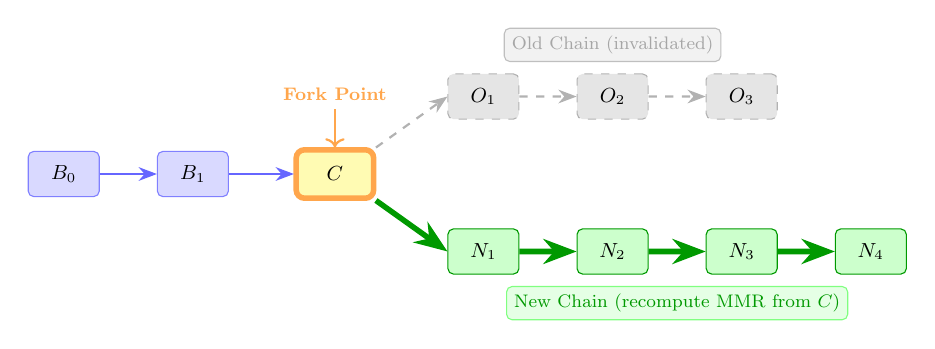
\begin{tikzpicture}[
    block/.style={rectangle, draw=blue!50, fill=blue!15, minimum width=1.1cm, minimum height=0.7cm, font=\small, rounded corners=2pt},
    oldblock/.style={rectangle, draw=gray!60, fill=gray!20, minimum width=1.1cm, minimum height=0.7cm, font=\small, rounded corners=2pt, dashed},
    newblock/.style={rectangle, draw=green!60!black, fill=green!20, minimum width=1.1cm, minimum height=0.7cm, font=\small, rounded corners=2pt},
    common/.style={rectangle, draw=orange!70, fill=yellow!30, minimum width=1.2cm, minimum height=0.75cm, font=\small\bfseries, line width=2pt, rounded corners=3pt},
    arrow/.style={->, >=Stealth, thick},
    scale=0.82, transform shape
]
    % Common chain
    \node[block] (b0) at (0,0) {$B_0$};
    \node[block] (b1) at (2,0) {$B_1$};
    \node[common] (c) at (4.2,0) {$C$};
    
    % Old chain (top, faded)
    \node[oldblock] (old1) at (6.5,1.2) {$O_1$};
    \node[oldblock] (old2) at (8.5,1.2) {$O_2$};
    \node[oldblock] (old3) at (10.5,1.2) {$O_3$};
    
    % New chain (bottom, emphasized)
    \node[newblock] (new1) at (6.5,-1.2) {$N_1$};
    \node[newblock] (new2) at (8.5,-1.2) {$N_2$};
    \node[newblock] (new3) at (10.5,-1.2) {$N_3$};
    \node[newblock] (new4) at (12.5,-1.2) {$N_4$};
    
    % Arrows - common chain
    \draw[arrow, blue!60] (b0) -- (b1);
    \draw[arrow, blue!60] (b1) -- (c);
    
    % Arrows - old chain (dashed, gray)
    \draw[arrow, dashed, gray!60, line width=0.8pt] (c.north east) -- (old1.west);
    \draw[arrow, dashed, gray!60, line width=0.8pt] (old1) -- (old2);
    \draw[arrow, dashed, gray!60, line width=0.8pt] (old2) -- (old3);
    
    % Arrows - new chain (thick, green)
    \draw[arrow, line width=2pt, green!60!black] (c.south east) -- (new1.west);
    \draw[arrow, line width=2pt, green!60!black] (new1) -- (new2);
    \draw[arrow, line width=2pt, green!60!black] (new2) -- (new3);
    \draw[arrow, line width=2pt, green!60!black] (new3) -- (new4);
    
    % Labels in boxes
    \node[draw=gray!50, fill=gray!10, rounded corners=2pt, font=\footnotesize, text=gray!70] at (8.5,2) {Old Chain (invalidated)};
    \node[draw=green!50, fill=green!10, rounded corners=2pt, font=\footnotesize, text=green!60!black] at (9.5,-2) {New Chain (recompute MMR from $C$)};
    
    % Fork point indicator
    \draw[<-, thick, orange!70] (c.north) -- ++(0,0.6) node[above, font=\footnotesize\bfseries, text=orange!70] {Fork Point};
\end{tikzpicture}
\caption{Chain reorganization handling. MMR state is retrieved from common ancestor $C$, and new chain blocks have their MMR states recomputed forward.}
\label{fig:reorg}
\end{figure}

To handle this:
\begin{itemize}
    \item We maintain the MMR state per block (peaks and size) in our store
    \item During reorg, we find $C$ (the common ancestor) and retrieve $C$'s MMR state
    \item We iterate forward from $C$ along the new selected chain, recomputing the MMR state for each block
\end{itemize}

Reorg handling is $\bigO(k)$ where $k$ is the number of blocks switched, typically small.

\subsection{Reorg Window and Checkpoint Policy}
\label{sec:reorg-checkpoint}

We parameterize the protocol's treatment of reorganization and finality:

\begin{definition}[Protocol Parameters]
\label{def:protocol-params}
\begin{itemize}
    \item $K_{\text{reorg}}$: \textbf{Reorg Bound} --- maximum expected reorganization depth (blocks). Beyond this, proofs are considered ``practically final.'' Typical value: 3,600 blocks ($\sim$6 minutes at 10 BPS).
    \item $T_{\text{checkpoint}}$: \textbf{Checkpoint Period} --- interval between rolling checkpoints. Typical value: 86,400 blocks ($\sim$24 hours at 10 BPS).
    \item $K_{\text{finality}}$: \textbf{Finality Depth} --- depth at which a block is considered irreversible for practical purposes. Often aligned with $K_{\text{reorg}}$.
\end{itemize}
\end{definition}

\textbf{Theoretical Basis for $K_{\text{reorg}}$:}
The parameter $K_{\text{reorg}}$ is chosen based on GHOSTDAG's security analysis. Under standard PoW assumptions, the probability of a $k$-depth reorganization decreases exponentially with $k$. Following the analysis in~\cite{ghostdag}, the probability of a reorganization at depth $k$ is bounded by $e^{-\Omega(k)}$.

For practical security, we set $K_{\text{reorg}}$ such that the reorganization probability is below $2^{-40}$ (approximately $10^{-12}$). For GHOSTDAG with typical network parameters, this corresponds to $K_{\text{reorg}} \approx 3,600$ blocks at 10 BPS, providing a conservative bound that ensures proofs beyond this depth are ``practically final'' in the same sense that block confirmations are final under standard PoW security assumptions.

\textbf{Proof Validity Windows:}
\begin{enumerate}
    \item \textbf{Within $K_{\text{reorg}}$:} Proofs may become invalid due to reorganization. L2 systems \rfc{should} wait $K_{\text{reorg}}$ confirmations before treating a proof as final, or be prepared to re-request updated proofs.
    \item \textbf{Beyond $K_{\text{reorg}}$:} Proofs are ``practically final''---reorganization of this depth would require attacking the consensus itself.
    \item \textbf{Beyond $T_{\text{checkpoint}}$:} If rolling is used, nodes may need pre-generated proofs or archive node services.
\end{enumerate}

\textbf{Checkpoint Alignment:} For optimal interoperability, checkpoints \rfc{should} align with protocol-level posterity headers (if any). This enables:
\begin{itemize}
    \item Consistent proof composability across nodes
    \item Known anchor points for historical verification
    \item Simplified disaster recovery procedures
\end{itemize}

\begin{longtable}{@{}lllp{5cm}@{}}
\caption{Recommended Protocol Parameters (10 BPS)}
\label{tab:protocol-params} \\
\small
\toprule
\textbf{Parameter} & \textbf{Value} & \textbf{Time} & \textbf{Rationale} \\
\midrule
\endfirsthead
\multicolumn{4}{c}{{\bfseries \tablename\ \thetable{} -- continued from previous page}} \\
\toprule
\textbf{Parameter} & \textbf{Value} & \textbf{Time} & \textbf{Rationale} \\
\midrule
\endhead
\midrule \multicolumn{4}{r}{{Continued on next page}} \\
\endfoot
\bottomrule
\endlastfoot
$K_{\text{reorg}}$ & 3,600 & $\sim$6 min & Conservative reorg bound \\
$K_{\text{finality}}$ & 3,600 & $\sim$6 min & Aligned with reorg bound \\
$T_{\text{checkpoint}}$ & 86,400 & $\sim$24 hr & Aligned with pruning period \\
\end{longtable}

\subsection{MMR Node Storage (Enabling Proof Generation)}

While the peaks alone are enough for consensus validation (we just need to recompute the new root), generating an actual inclusion proof for an arbitrary past block or transaction requires access to the intermediate nodes (siblings along the path). A full node that wants to support light clients or bridges with proofs should maintain an \textbf{MMR Node Store} mapping each node position to its hash.

\textbf{Indexing Scheme:} The positions can be indexed by a single number if we linearize the MMR tree in a certain traversal. A simple scheme is:
\begin{itemize}
    \item Label the leaves with indices starting from 0
    \item Label internal nodes in the order they are created during the append process
    \item The position of a node can be derived from the leaf index and the node's height
\end{itemize}

We store each node hash keyed by its position. To produce a proof for leaf $i$, we:
\begin{enumerate}
    \item Compute the positions of each sibling on the path from that leaf to the peak
    \item Retrieve those sibling hashes from the store
    \item Also retrieve the peak hashes
\end{enumerate}
All of this is $\bigO(\log n)$ operations.

\textbf{Storage Cost:} Each leaf or internal node is one hash (32 bytes). An MMR with $n$ leaves has $< 2n$ nodes in total (similar to a full binary tree). The node store size for $n$ leaves is roughly $2n \times 32$ bytes:
\begin{itemize}
    \item After 1,000,000 leaves: $2 \times 10^6 \times 32 = 64$ MB
    \item After 300,000,000 leaves ($\sim$1 year at 10 BPS): $\sim$19.2 GB
\end{itemize}
This is within reason for a well-resourced node serving many light clients.

\textbf{Recommended Storage Practice:} For a full node at 10 BPS:
\begin{enumerate}
    \item Store all block headers permanently (few tens of GB/year)---required for consensus
    \item Maintain an MMR node store persistently ($\sim$20 GB/year) if supporting historical proofs
    \item Maintain a rolling cache of peaks for recent blocks (last day or week) for fast reorg handling. For example, 86,400 blocks for a day at 10 BPS with $\sim$20 peaks each $\approx$ 55 MB
\end{enumerate}

\subsection{Pruning and Checkpointing}

GHOSTDAG nodes may prune old blocks, but they typically keep all headers (including the MMR fields). Thus, a pruned node can still verify a proof of inclusion for a pruned block: it has that block's header and the tip header.

A headers-only node can verify inclusion of a transaction from any block, given a correct proof. This is by design: enabling light clients to be almost as secure as full nodes for checking inclusion, without storing everything. The MMR commitment turns the whole history into a \emph{self-authenticating log}: the node can verify any historical data from an untrusted source against the known \code{elog\_root}.

\subsection{Rolling MMR for Long-Term Scalability}
\label{sec:rolling-mmr}

While an append-only MMR provides excellent properties for historical verification, the unbounded growth of the MMR poses long-term storage challenges. At 10 BPS, the MMR node store grows at approximately 20 GB per year. Over decades, this becomes significant even for well-resourced nodes. We propose a \textbf{Rolling MMR} mechanism to address this.

\textbf{Critical Invariant:} Rolling is a \emph{storage optimization only}---it does not alter consensus commitments. The \code{elog\_root} in block headers is always computed from the full MMR (conceptually from genesis), regardless of what a particular node stores locally.

\begin{quote}
\textit{``Rolling does not alter consensus commitments; it only affects the availability of historical witnesses.''}
\end{quote}

\subsubsection{Checkpoint-Based MMR Rolling}

Rather than maintaining the complete MMR from genesis indefinitely, nodes can periodically ``roll forward'' the MMR base:

\begin{enumerate}
    \item \textbf{Checkpoint Selection:} At regular intervals (e.g., every pruning epoch, approximately 24 hours), designate a checkpoint block $B_c$ on the selected parent chain
    \item \textbf{MMR State Snapshot:} Store the complete MMR peaks at $B_c$ as a \emph{frozen checkpoint}
    \item \textbf{Prefix Pruning:} Old MMR nodes (those corresponding to leaves before $B_c$) can be pruned, keeping only:
    \begin{itemize}
        \item The frozen checkpoint state (peaks and size at $B_c$)
        \item Recent MMR nodes (from $B_c$ onward)
    \end{itemize}
\end{enumerate}

\textbf{Consensus Remains Unaffected:} A node that has rolled its MMR can still:
\begin{itemize}
    \item Validate new blocks (only requires parent's MMR state, which is recent)
    \item Compute \code{elog\_root} correctly (same algorithm, same result)
    \item Participate fully in consensus
\end{itemize}

What the node \emph{cannot} do after rolling is generate proofs for blocks before the checkpoint. This is a data availability limitation, not a consensus limitation.

\subsubsection{Proof Generation with Rolling MMR}

For transactions in blocks \emph{after} the checkpoint $B_c$, proof generation works normally using the local MMR store.

For transactions in blocks \emph{before} $B_c$:
\begin{itemize}
    \item The proving node must either (a) have retained the full historical MMR, or (b) request the historical proof from an archive node
    \item The proof can be composed: a proof from the old transaction to the checkpoint's MMR root, plus a proof from the checkpoint to the current tip
    \item Alternatively, users who need long-term proofs should generate and store them \emph{before} the relevant MMR nodes are pruned
\end{itemize}

\textbf{Checkpoint Verifiability:} A checkpoint snapshot (peaks list and size at block $B_c$) must be verifiable against the on-chain commitment. The checkpoint is identified by block header $B_c$, which contains \code{elog\_root} and \code{elog\_size}. To verify a checkpoint snapshot:

\begin{enumerate}
    \item Retrieve block header $B_c$ (already in the headers chain, protected by PoW)
    \item Extract \code{elog\_root} and \code{elog\_size} from $B_c$
    \item Recompute the MMR root from the checkpoint snapshot (peaks and size):
    \begin{itemize}
        \item Bag all peaks: $\text{bag} = \text{bag\_peaks}(\text{checkpoint.peaks})$
        \item Compute root: $\text{computed\_root} = \Hroot(\text{DOMAIN\_ROOT} \parallel \text{bag} \parallel \text{encode}_{64}(\text{checkpoint.size}))$
    \end{itemize}
    \item Verify: $\text{computed\_root} = B_c.\text{elog\_root}$ and $\text{checkpoint.size} = B_c.\text{elog\_size}$
\end{enumerate}

If verification passes, the checkpoint snapshot is cryptographically bound to the on-chain state at $B_c$. This ensures that rolling does not introduce trust assumptions beyond the blockchain's own security.

\textbf{Proof Composability:} A key property of MMR proofs is that they can be \emph{spliced} across checkpoints. Given:
\begin{itemize}
    \item Proof $\pi_1$: transaction $\to$ \code{elog\_root} at checkpoint $C_1$ (verified against $B_{C_1}$)
    \item Proof $\pi_2$: checkpoint $C_1$'s state $\to$ \code{elog\_root} at checkpoint $C_2$ (verified against $B_{C_2}$)
\end{itemize}
A verifier holding \code{elog\_root} at $C_2$ can verify the transaction by composing $\pi_1$ and $\pi_2$. This enables a hierarchical proof ecosystem where archive nodes store proof segments and users compose them on demand. The checkpoint's verifiability ensures that proof composition maintains the same security guarantees as a single proof from genesis.

\subsubsection{Node Capability Tiers}

Rolling creates a natural tiering of node capabilities:

\begin{center}
\begin{tabular}{lcc}
\toprule
\textbf{Node Type} & \textbf{Consensus Participation} & \textbf{Proof Generation} \\
\midrule
Pruned Node & Full & None (no MMR nodes stored) \\
Rolling Node & Full & Recent blocks only \\
Archive Node & Full & All historical blocks \\
\bottomrule
\end{tabular}
\end{center}

All node types participate equally in consensus. The difference is purely in their ability to \emph{serve proofs} to external parties.

\subsubsection{Storage Trade-offs}

\begin{center}
\begin{tabular}{lcc}
\toprule
\textbf{Strategy} & \textbf{Storage (per year)} & \textbf{Proof Availability} \\
\midrule
Full MMR (no rolling) & $\sim$20 GB/year cumulative & All historical proofs \\
Daily checkpoints & $\sim$500 MB/year & Recent + checkpoint-based \\
Weekly checkpoints & $\sim$100 MB/year & Recent + archived \\
\bottomrule
\end{tabular}
\end{center}

The rolling approach is optional: archive nodes can maintain the complete MMR history, while regular nodes use rolling to bound storage. This mirrors how GHOSTDAG implementations already handle block body pruning---the MMR commitment in headers enables verification even when underlying data is pruned, as long as proofs were generated before pruning.

\subsubsection{Proof Availability: Formal Model}
\label{sec:rolling-semantics}

We now formalize the proof availability guarantees, distinguishing between \textbf{protocol guarantees} and \textbf{economic/social assumptions}.

\begin{definition}[Verification vs. Generation]
\label{def:verify-vs-generate}
\begin{itemize}
    \item \textbf{Proof Verification:} Given a proof $\pi$ and trusted \code{elog\_root}, determine if $\pi$ is valid. Requires only the proof data and header.
    \item \textbf{Proof Generation:} Given a transaction $tx$ and block $B$, produce a valid proof $\pi$. Requires access to MMR internal nodes.
\end{itemize}
\textbf{Key Property:} Verification is always possible given valid proof data; generation depends on data availability.
\end{definition}

\begin{definition}[Availability Models]
\label{def:availability-models}
We define two availability models:

\textbf{Model A: Bounded-History Verification (Protocol Guarantee)}
\begin{itemize}
    \item For blocks within the last $T_{\text{checkpoint}}$ blocks ($\sim$24 hours), all full nodes \rfc{can} generate proofs
    \item This is a \textbf{protocol guarantee}: the protocol specifies minimum retention
    \item Light clients can obtain proofs for recent transactions from any full node
\end{itemize}

\textbf{Model B: Historical Verification (Economic Assumption)}
\begin{itemize}
    \item For blocks older than $T_{\text{checkpoint}}$, proof generation requires archive nodes
    \item This is an \textbf{economic assumption}: at least one honest archive node is online and reachable
    \item The protocol does \emph{not} guarantee proof availability for historical blocks
\end{itemize}
\end{definition}

\begin{longtable}{@{}p{2.5cm}p{3cm}p{3cm}p{4cm}@{}}
\caption{Proof Availability Guarantees}
\label{tab:proof-availability} \\
\small
\toprule
\textbf{Block Age} & \textbf{Proof Generation} & \textbf{Guarantee Type} & \textbf{Failure Mode} \\
\midrule
\endfirsthead
\multicolumn{4}{c}{{\bfseries \tablename\ \thetable{} -- continued from previous page}} \\
\toprule
\textbf{Block Age} & \textbf{Proof Generation} & \textbf{Guarantee Type} & \textbf{Failure Mode} \\
\midrule
\endhead
\midrule \multicolumn{4}{r}{{Continued on next page}} \\
\endfoot
\bottomrule
\endlastfoot
$< T_{\text{checkpoint}}$ & Any full node & Protocol & None (guaranteed) \\
$\geq T_{\text{checkpoint}}$ & Archive nodes only & Economic & No archive online $\Rightarrow$ no new proofs \\
Any age & --- & --- & Pre-generated proofs remain valid forever \\
\end{longtable}

\begin{theorem}[Proof Availability Separation]
\label{thm:availability-separation}
The execution log scheme separates \textbf{consensus commitments} (always verifiable) from \textbf{proof generation capability} (availability-dependent):

\begin{enumerate}
    \item \textbf{Commitment Persistence:} The \code{elog\_root} in block headers is a permanent, on-chain commitment. It can be verified against any valid proof, regardless of when the proof was generated or by whom.
    
    \item \textbf{Generation Availability:} Proof generation for block $B$ requires access to MMR internal nodes. For blocks within $T_{\text{checkpoint}}$, this is protocol-guaranteed (all full nodes retain the data). For older blocks, this depends on archive node availability (economic assumption).
    
    \item \textbf{Verification Independence:} Proof verification does \emph{not} depend on proof generation capability. A verifier can validate a proof even if no node can currently generate new proofs for that block.
\end{enumerate}
\end{theorem}

\textbf{Proof Sketch:}
\begin{enumerate}
    \item \textbf{Commitment persistence:} The \code{elog\_root} is stored in block headers, which are retained indefinitely (required for consensus). Verification only requires the proof data and the header's \code{elog\_root}.
    
    \item \textbf{Generation availability:} MMR internal nodes are not required for consensus (only peaks are needed for root computation). Nodes may prune internal nodes to save storage. This affects generation capability, not verification.
    
    \item \textbf{Verification independence:} Verification algorithm (Algorithm~\ref{alg:proof-verify}) requires only: proof data, block headers, and hash function. It does not require MMR internal nodes.
\end{enumerate}
\qed

\begin{corollary}[Rolling Compatibility]
\label{cor:rolling-compatible}
Rolling MMR (pruning internal nodes while retaining checkpoints) is \textbf{consensus-compatible}: it does not affect the ability to verify proofs, only the ability to generate new proofs for pruned blocks.
\end{corollary}

This separation enables a \textbf{capability tier model} where different node types provide different services (consensus participation, recent proof generation, historical proof generation) while maintaining the same security guarantees for verification.

\subsubsection{Node Capability Tiers}

\begin{definition}[Node Capability Classes]
\label{def:node-capabilities}
\begin{enumerate}
    \item \textbf{Archive Node:} Stores complete MMR from genesis. Can generate proofs for any block. Storage: $\sim$20 GB/year.
    \item \textbf{Full Node (Rolling):} Stores MMR state from last checkpoint. Can generate proofs for recent blocks, verify any proof. Storage: bounded.
    \item \textbf{Light Node:} Stores only headers. Can verify proofs, cannot generate them.
\end{enumerate}
\end{definition}

\subsubsection{Minimum Data Retention Requirements}

\begin{itemize}
    \item \rfc{MUST} retain: All block headers (including \code{exec\_root}, \code{elog\_root}, \code{elog\_size})---required for consensus
    \item \rfc{MUST} retain: MMR peaks at each checkpoint (for proof composability across checkpoints)
    \item \rfc{SHOULD} retain: MMR internal nodes for last $T_{\text{checkpoint}}$ blocks (for proof generation)
    \item \rfc{MAY} prune: MMR internal nodes for blocks before checkpoint
    \item \rfc{MAY} prune: Block bodies per existing pruning rules
\end{itemize}

\subsubsection{Failure Modes and Mitigations}

\textbf{Failure Mode 1: No archive node available}
\begin{itemize}
    \item \textbf{Impact:} Cannot generate new proofs for blocks older than $T_{\text{checkpoint}}$
    \item \textbf{Mitigation:} Pre-generate and cache proofs for important transactions before pruning
    \item \textbf{Recovery:} If \emph{any} archive comes online later, historical proofs become available again
\end{itemize}

\textbf{Failure Mode 2: Malicious archive provides invalid proof}
\begin{itemize}
    \item \textbf{Impact:} None---light client can detect and reject invalid proofs via verification
    \item \textbf{Property:} Archives cannot forge proofs; they can only refuse to serve
\end{itemize}

\textbf{Failure Mode 3: Light client cannot find any proof source}
\begin{itemize}
    \item \textbf{Impact:} Proof retrieval fails (data availability issue, not security issue)
    \item \textbf{Mitigation:} Multiple independent archives, incentivized proof services
\end{itemize}

\subsubsection{Economic Incentives (Out of Scope)}

We note that a complete system may include economic incentives for archive operation:
\begin{itemize}
    \item Proof generation fees paid to archive operators
    \item Staking/slashing for archive availability guarantees
    \item Protocol-level archival rewards
\end{itemize}
These mechanisms are \textbf{outside the scope} of this paper. Our contribution is the cryptographic scheme; incentive design is left to implementation.

%==============================================================================
% SECTION 5: PROOFS
%==============================================================================
\section{Inclusion Proofs and Verification}
\label{sec:proofs}

A major goal of this design is to enable efficient transaction inclusion proofs that a light client or smart contract can verify.

\subsection{Two-Layer Proof Model}
\label{sec:what-exactly-proven}

To prove that a transaction $tx$ was \textbf{executed at a specific position} in the global execution order, we provide a two-layer proof structure:

\begin{enumerate}
    \item \textbf{Intra-Block Execution Proof:} Proves $tx$ was executed at position $i$ within block $B$'s accepted transaction list ($0 \leq i < |\text{AcceptedTxList}(B)|$)
    \item \textbf{Inter-Block MMR Inclusion Proof:} Proves block $B$'s execution commitment is at leaf index $j$ in the execution log MMR ($j = $ block's position in selected chain)
\end{enumerate}

\subsubsection{What Exactly Is Proven?}

We are precise about what the proof establishes:

\begin{proposition}[Execution Position Proof]
\label{prop:execution-position}
A valid two-layer proof establishes the following statement:
\begin{quote}
``Transaction $tx$ is the $i$-th executed transaction in block $B$, where block $B$ is the $j$-th block in the selected parent chain (with $j = \text{leaf\_index}$).''
\end{quote}
This gives a \textbf{hierarchical position} $(j, i)$: block index $j$, intra-block index $i$.
\end{proposition}

\textbf{Important Clarification:} The proof does \emph{not} directly establish a ``global transaction index'' (e.g., ``the 1,234,567-th transaction ever executed''). Computing such an index would require knowing the cumulative transaction count up to block $j-1$, which is not committed in our current scheme.

\textbf{Options for Global Indexing (if needed):}
\begin{enumerate}
    \item \textbf{Prefix-Sum Commitment:} Add a \code{cum\_tx\_count} field to each block header, committing the total transactions executed up to (and including) that block. Then global index $= \text{cum\_tx\_count}(j-1) + i$.
    \item \textbf{Encode Count in Leaf:} Extend the MMR leaf to include block's transaction count: $L(B) = H_{\text{leaf}}(\text{parent\_hash} \| \text{exec\_root} \| |\text{AcceptedTxList}|)$. A verifier can sum counts along the proof path.
    \item \textbf{Accept Hierarchical Position:} For many L2 use cases, $(j, i)$ is sufficient---L2 contracts can maintain their own mapping if needed.
\end{enumerate}

For this paper, we adopt option (3): the hierarchical position $(j, i)$ is the canonical proof output. This keeps the scheme minimal while remaining sufficient for most applications (transaction ordering, dispute resolution, bridge verification).

This two-layer structure is the \textbf{minimal proof} that an L2 system needs to verify execution position. It is more powerful than skip-list chain membership proofs (which only prove block inclusion) and more efficient than linear chain traversal (which requires $\bigO(n)$ operations).

\begin{figure}[htbp]
\centering
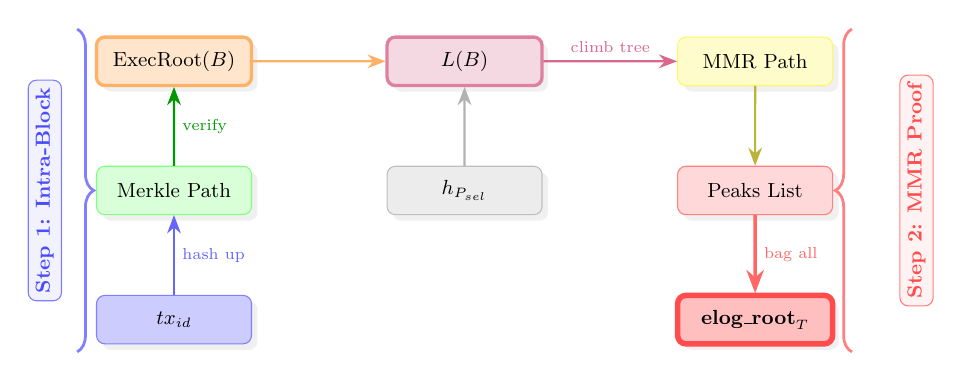
\begin{tikzpicture}[
    box/.style={rectangle, draw, rounded corners=3pt, minimum width=2.4cm, minimum height=0.75cm, font=\small, drop shadow={opacity=0.12}},
    arrow/.style={->, >=Stealth, thick},
    scale=0.82, transform shape
]
    % Step 1: Intra-Block (left column)
    \node[box, fill=blue!20, draw=blue!50] (tx) at (0,0) {$tx_{id}$};
    \node[box, fill=green!15, draw=green!50] (merkle) at (0,2) {Merkle Path};
    \node[box, fill=orange!20, draw=orange!60, line width=1.2pt] (order) at (0,4) {$\ExecRoot(B)$};
    
    % Middle column (leaf computation)
    \node[box, fill=purple!15, draw=purple!50, line width=1.2pt] (leaf) at (4.5,4) {$L(B)$};
    \node[box, fill=gray!15, draw=gray!50] (parent) at (4.5,2) {$h_{P_{sel}}$};
    
    % Step 2: MMR (right column)
    \node[box, fill=yellow!20, draw=yellow!60] (mmrpath) at (9,4) {MMR Path};
    \node[box, fill=red!15, draw=red!50] (peaks) at (9,2) {Peaks List};
    \node[box, fill=red!25, draw=red!70, line width=2pt, font=\small\bfseries] (mmrroot) at (9,0) {$\text{elog\_root}_T$};
    
    % Arrows with labels
    \draw[arrow, blue!60] (tx) -- node[right, font=\scriptsize, text=blue!60] {hash up} (merkle);
    \draw[arrow, green!60!black] (merkle) -- node[right, font=\scriptsize, text=green!60!black] {verify} (order);
    \draw[arrow, orange!60] (order) -- (leaf);
    \draw[arrow, gray!60] (parent) -- (leaf);
    \draw[arrow, purple!60] (leaf) -- node[above, font=\scriptsize, text=purple!60] {climb tree} (mmrpath);
    \draw[arrow, yellow!70!black] (mmrpath) -- (peaks);
    \draw[arrow, red!60, line width=1.2pt] (peaks) -- node[right, font=\scriptsize, text=red!60] {bag all} (mmrroot);
    
    % Step labels with boxes
    \node[draw=blue!50, fill=blue!5, rounded corners=3pt, font=\small\bfseries, text=blue!70, rotate=90, minimum width=3cm] at (-2,2) {Step 1: Intra-Block};
    
    \node[draw=red!50, fill=red!5, rounded corners=3pt, font=\small\bfseries, text=red!70, rotate=90, minimum width=3cm] at (11.5,2) {Step 2: MMR Proof};
    
    % Decorative braces
    \draw[decorate, decoration={brace, amplitude=6pt, mirror}, blue!50, line width=1pt] (-1.5,-0.5) -- (-1.5,4.5);
    \draw[decorate, decoration={brace, amplitude=6pt}, red!50, line width=1pt] (10.5,-0.5) -- (10.5,4.5);
\end{tikzpicture}
\caption{Two-step proof verification process. Step 1 verifies the transaction is in block $B$ via Merkle proof. Step 2 verifies block $B$ is in the MMR via MMR proof.}
\label{fig:proof-verification}
\end{figure}

We formalize a proof as a tuple $(txId, B, \text{IntraProof}, \text{MMRProof}, T)$ where:
\begin{itemize}
    \item $txId$ is the transaction identifier (hash) we are proving
    \item $B$ is the block hash in which $tx$ was included
    \item $\text{IntraProof}$ contains the Merkle path nodes needed to compute $B$'s $\ExecRoot$ from $txId$
    \item $\text{MMRProof}$ contains the MMR leaf index, sibling hashes, and peaks list
    \item $T$ is the block hash whose MMR root we are anchoring to
\end{itemize}

\textbf{Intra-Block Merkle Proof Format:} This is the classic Merkle branch: given the index of the transaction in the block and the Merkle root (\code{exec\_root}) from the block header, provide the sibling hashes at each level:
\begin{lstlisting}[language=Python,caption=Intra-Block Proof Structure]
IntraProof = {
    tx_index: u32,              # Position in TxList
    siblings: [(Hash, bool)],   # (sibling_hash, is_left)
}
\end{lstlisting}

\textbf{MMR Inclusion Proof Format (Route A: Explicit Side Indicators):}
\begin{lstlisting}[language=Python,caption=MMR Proof Structure]
MMRProof = {
    leaf_index: u64,            # 0-based leaf index in selected chain
    elog_size: u64,             # MMR size at proof time
    path: [(Hash, Side)],       # Path from leaf to peak: (sibling_hash, is_left)
    peak_index: u8,             # Index of target peak in peaks list (0-based)
    peaks: [Hash],              # All peak hashes (ordered left-to-right)
    parent_hash: Hash,          # B's selected parent hash
    exec_root: Hash,            # B's exec_root
}
\end{lstlisting}

where \code{Side} is a boolean: \code{True} means sibling is on the left (current is right child), \code{False} means sibling is on the right (current is left child).

\textbf{Byte-Level Layout (TLV-style):}
\begin{itemize}
    \item \code{leaf\_index}: 8 bytes, little-endian u64
    \item \code{elog\_size}: 8 bytes, little-endian u64
    \item \code{path\_length}: 1 byte, u8 (number of path steps)
    \item \code{path}: \code{path\_length} $\times$ (32 bytes hash + 1 byte side flag)
    \item \code{peak\_index}: 1 byte, u8
    \item \code{peaks\_count}: 1 byte, u8
    \item \code{peaks}: \code{peaks\_count} $\times$ 32 bytes
    \item \code{parent\_hash}: 32 bytes
    \item \code{exec\_root}: 32 bytes
\end{itemize}

Total size: $8 + 8 + 1 + \text{path\_length} \times 33 + 1 + 1 + \text{peaks\_count} \times 32 + 32 + 32$ bytes. For typical proofs (path length $\sim$20, peaks count $\sim$5), this is approximately 1 KB.

\textbf{Proof Size Optimization: Peak Compression}

The \code{peaks} field contains all MMR peak hashes. For a chain with $n$ blocks, there are at most $\lceil \log_2 n \rceil$ peaks. At 10 BPS over 10 years ($\sim$3 billion blocks), this is $\sim$32 peaks $\times$ 32 bytes $= 1$ KB.

For further optimization, implementations \rfc{may} use one of:

\begin{enumerate}
    \item \textbf{Full Peaks (Default):} Include all peak hashes. Simple, slightly larger proofs.
    
    \item \textbf{Bagged Peaks Root:} The verifier already knows \code{elog\_root}, which is derived from peaks. The proof includes only peaks \emph{not} on the verification path. The verifier reconstructs missing peaks during path computation.
    
    \item \textbf{Compressed Peaks Commitment:} Store a Merkle root of peaks in the proof; include Merkle proof for needed peaks. Trades computation for bandwidth.
\end{enumerate}

For this paper, we use option (1) for simplicity. The proof size difference is marginal ($\sim$500 bytes), and full peaks simplify verification logic.

\begin{algorithm}[htbp]
\caption{Complete Proof Verification}
\label{alg:proof-verify}
\begin{algorithmic}[1]
\Require Transaction ID $txId$, IntraProof, MMRProof, trusted $\text{elog\_root}_T$
\Ensure Proof validity (true/false)

\State \textbf{Step 1: Verify Transaction in Block}
\State hash $\gets txId$
\For{(sibling, is\_left) in IntraProof.siblings}
    \If{is\_left}
        \State hash $\gets H(\text{sibling} \parallel \text{hash})$
    \Else
        \State hash $\gets H(\text{hash} \parallel \text{sibling})$
    \EndIf
\EndFor
\If{hash $\neq$ MMRProof.exec\_root}
    \State \Return \textsc{False}
\EndIf

\State \textbf{Step 2: Compute MMR Leaf}
\State leaf $\gets \Hleaf(\text{DOMAIN\_LEAF} \parallel \text{MMRProof.parent\_hash} \parallel \text{MMRProof.exec\_root})$

\State \textbf{Step 3: Verify MMR Path to Peak}
\State current $\gets$ leaf
\For{(sibling, is\_left) in MMRProof.path}
    \If{is\_left}  \Comment{Sibling is left, current is right child}
        \State current $\gets \Hnode(\text{DOMAIN\_NODE} \parallel \text{sibling} \parallel \text{current})$
    \Else  \Comment{Sibling is right, current is left child}
        \State current $\gets \Hnode(\text{DOMAIN\_NODE} \parallel \text{current} \parallel \text{sibling})$
    \EndIf
\EndFor
\State computed\_peak $\gets$ current
\If{computed\_peak $\neq$ MMRProof.peaks[MMRProof.peak\_index]}
    \State \Return \textsc{False}  \Comment{Path does not lead to claimed peak}
\EndIf

\State \textbf{Step 4: Verify Peak Bagging and Root}
\If{MMRProof.peaks is empty}
    \State \Return \textsc{False}
\EndIf
\State bag $\gets$ MMRProof.peaks[0]
\For{$i \gets 1$ to $\text{len}(\text{MMRProof.peaks}) - 1$}
    \State bag $\gets \Hbag(\text{DOMAIN\_BAG} \parallel \text{bag} \parallel \text{MMRProof.peaks}[i])$
\EndFor
\State expected\_root $\gets \Hroot(\text{DOMAIN\_ROOT} \parallel \text{bag} \parallel \text{encode}_{64}(\text{MMRProof.elog\_size}))$
\If{expected\_root $\neq$ $\text{elog\_root}_T$}
    \State \Return \textsc{False}
\EndIf
\State \Return \textsc{True}
\end{algorithmic}
\end{algorithm}

\subsection{Proof Size and Efficiency}

\begin{theorem}[Proof Size Bound]
For a transaction in block $B$ with $m$ transactions, and MMR with $N$ leaves, the total proof size is:
\begin{equation}
\text{ProofSize} = \bigO(\log m + \log N) \times 32 \text{ bytes}
\end{equation}
\end{theorem}

\begin{longtable}{@{}rrrrr@{}}
\caption{Proof Size Estimates for Various Chain Lengths at 10 BPS}
\label{tab:proof-size} \\
\toprule
\textbf{Chain Length} & \textbf{Time} & \textbf{MMR Depth} & \textbf{Est. Proof Size} & \textbf{Verification Hashes} \\
\midrule
\endfirsthead
\multicolumn{5}{c}{{\bfseries \tablename\ \thetable{} -- continued from previous page}} \\
\toprule
\textbf{Chain Length} & \textbf{Time} & \textbf{MMR Depth} & \textbf{Est. Proof Size} & \textbf{Verification Hashes} \\
\midrule
\endhead
\midrule \multicolumn{5}{r}{{Continued on next page}} \\
\endfoot
\bottomrule
\endlastfoot
$10^6$ blocks & $\sim$1 day & 20 & $\sim$800 bytes & $\sim$25 \\
$10^7$ blocks & $\sim$12 days & 24 & $\sim$900 bytes & $\sim$30 \\
$10^8$ blocks & $\sim$4 months & 27 & $\sim$1.0 KB & $\sim$35 \\
$3 \times 10^8$ blocks & $\sim$1 year & 28 & $\sim$1.1 KB & $\sim$40 \\
\end{longtable}

This represents a significant improvement over a linear chain proof, which would require every block header hash in between (tens of kilobytes or more for deep history).

\begin{longtable}{@{}rrrr@{}}
\caption{Proof Size (Hash Operations) vs Age of Transaction}
\label{tab:proof-comparison} \\
\toprule
\textbf{Blocks Ago ($d$)} & \textbf{Linear Hash Ops} & \textbf{MMR Hash Ops} & \textbf{Improvement} \\
\midrule
\endfirsthead
\multicolumn{4}{c}{{\bfseries \tablename\ \thetable{} -- continued from previous page}} \\
\toprule
\textbf{Blocks Ago ($d$)} & \textbf{Linear Hash Ops} & \textbf{MMR Hash Ops} & \textbf{Improvement} \\
\midrule
\endhead
\midrule \multicolumn{4}{r}{{Continued on next page}} \\
\endfoot
\bottomrule
\endlastfoot
100 & $\sim$100 & $\sim$7--8 & 93\% fewer \\
1,000 & $\sim$1,000 & $\sim$10--11 & 99\% fewer \\
10,000 & $\sim$10,000 & $\sim$13--14 & 99.9\% fewer \\
100,000 & $\sim$100,000 & $\sim$17--18 & 99.98\% fewer \\
1,000,000 & $\sim$1,000,000 & $\sim$20--21 & 99.998\% fewer \\
\end{longtable}

Even at moderate distances like 10,000 blocks ($\sim$1,000 seconds at 10 BPS), the difference is stark: 10,000 vs $\sim$14 operations. This demonstrates that our approach is not just asymptotically better, but very practically so, enabling use cases that were completely out of reach before (e.g., verifying a 1-year old transaction on-chain is impossible linearly but easy with MMR).

\textbf{On-chain Verification Gas Costs:} For cross-chain bridge applications, on-chain verification cost is critical. Our scheme uses BLAKE3-256, but for cost estimation in EVM environments (which use Keccak-256), we provide approximate costs assuming similar per-hash gas consumption. Each hash operation costs approximately $\sim$1920 gas in EVM (for Keccak-256: $\sim 8 \text{ gas/byte} \times 64 \text{ bytes}$). The number of hash operations is the key factor; the specific hash function affects absolute cost but not the asymptotic advantage. Therefore:
\begin{itemize}
    \item MMR proof ($\sim$30 hashes): $\sim$57,600 gas---very manageable (typical ETH transfer costs $\sim$21,000 gas)
    \item Linear 100k hash proof: $\sim$192 million gas---exceeds block gas limit ($\sim$30M) by 6$\times$
\end{itemize}

\textbf{Batch Verification Advantage:} One great advantage of MMRs is that proofs for multiple leaves can share parts. If an L2 contract needs to verify $k$ transactions from possibly different blocks:
\begin{itemize}
    \item If from the same block: they share the entire MMR path
    \item If from different blocks: they share the peaks list
    \item Even 100 separate proofs might total only $\sim$3M gas, which is acceptable
\end{itemize}
This is crucial for verifying multiple withdrawals in one go on a bridge.

%==============================================================================
% SECTION 6: APPLICATIONS
%==============================================================================
\section{Applications and Benefits}
\label{sec:applications}

With the MMR execution-log accumulator in place, several important use cases become possible:

\subsection{Trustless Bridges and L2 Rollups}

\begin{figure}[htbp]
\centering
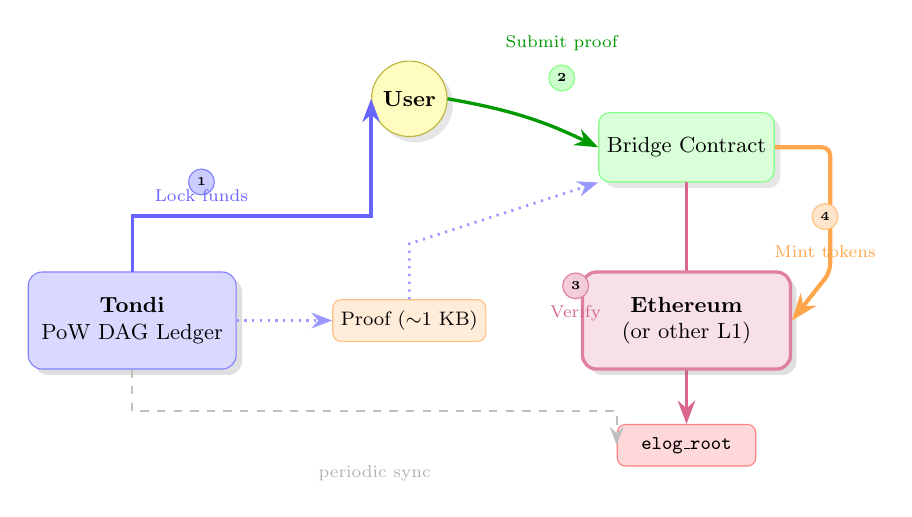
\begin{tikzpicture}[
    chain/.style={rectangle, draw, rounded corners=5pt, minimum width=3cm, minimum height=1.4cm, align=center, font=\small, drop shadow={opacity=0.25}},
    contract/.style={rectangle, draw, rounded corners=4pt, minimum width=2.4cm, minimum height=1cm, align=center, font=\small, drop shadow={opacity=0.2}},
    user/.style={circle, draw=yellow!70!black, fill=yellow!25, minimum size=1cm, font=\small\bfseries, drop shadow={opacity=0.2}},
    databox/.style={rectangle, draw, rounded corners=3pt, font=\footnotesize, minimum width=2cm, align=center, minimum height=0.6cm},
    arrow/.style={->, >=Stealth, thick},
    note/.style={font=\scriptsize},
    scale=0.88, transform shape
]
    % === LAYER 1: Background elements (drawn first) ===
    
    % Left side: Tondi (blue theme)
    \node[chain, fill=blue!15, draw=blue!50] (tondi) at (0,0) {\textbf{Tondi}\\PoW DAG Ledger};
    
    % Center: Proof box
    \node[databox, fill=orange!15, draw=orange!50] (proof) at (4,0) {Proof ($\sim$1 KB)};
    
    % MMR root storage
    \node[databox, fill=red!15, draw=red!50, font=\footnotesize\ttfamily] (mmr) at (8,-1.8) {elog\_root};
    
    % Bridge Contract
    \node[contract, fill=green!15, draw=green!50] (bridge) at (8,2.5) {Bridge Contract};
    
    % User
    \node[user] (user) at (4,3.2) {User};
    
    % === LAYER 2: Background arrows (drawn before Ethereum) ===
    
    % MMR sync arrow (gray, background)
    \draw[arrow, dashed, gray!50, line width=0.8pt] (tondi.south) -- ++(0,-0.6) -| (mmr.west);
    \node[note, text=gray!60] at (3.5,-2.2) {periodic sync};
    
    % Proof generation flow (dotted, background)
    \draw[arrow, dotted, blue!40, line width=1pt] (tondi.east) -- (proof.west);
    \draw[arrow, dotted, blue!40, line width=1pt] (proof.north) -- ++(0,0.8) -- (bridge.south west);
    
    % Step 1: Lock funds on L1
    \draw[arrow, blue!60, line width=1.2pt] (tondi.north) -- ++(0,0.8) -| (user.west);
    \node[circle, fill=blue!20, draw=blue!50, font=\tiny\bfseries, inner sep=2pt] at (1,2.0) {1};
    \node[note, text=blue!60] at (1,1.8) {Lock funds};
    
    % Step 2: Submit proof to bridge
    \draw[arrow, green!60!black, line width=1.2pt] (user.east) to[bend left=8] (bridge.west);
    \node[circle, fill=green!20, draw=green!50, font=\tiny\bfseries, inner sep=2pt] at (6.2,3.5) {2};
    \node[note, text=green!60!black] at (6.2,4) {Submit proof};
    
    % Step 3: Verify arrow (draw before Ethereum)
    \draw[arrow, purple!60, line width=1.2pt] (bridge.south) -- (mmr.north);
    
    % === LAYER 3: Ethereum in foreground (drawn on top) ===
    \node[chain, fill=purple!12, draw=purple!50, line width=1.2pt] (eth) at (8,0) {\textbf{Ethereum}\\(or other L1)};
    
    % Step 3 labels: drawn AFTER Ethereum so they appear on top
    \node[circle, fill=purple!20, draw=purple!50, font=\tiny\bfseries, inner sep=2pt] at (6.4,0.5) {3};
    \node[note, text=purple!60] at (6.4,0.1) {Verify};
    
    % Step 4: Mint tokens (elegant curved arrow going right)
    \draw[arrow, orange!70, line width=1.5pt, rounded corners=3pt] 
        (bridge.east) -- ++(0.8,0) -- ++(0,-1.8) -- (eth.east);
    \node[circle, fill=orange!20, draw=orange!50, font=\tiny\bfseries, inner sep=2pt] at (10.0,1.5) {4};
    \node[note, text=orange!70] at (10.0,1.0) {Mint tokens};
\end{tikzpicture}
\caption{Trustless bridge architecture using MMR proofs. The bridge contract stores only the latest \code{elog\_root} and verifies inclusion proofs on-chain with $\sim$30 hash operations.}
\label{fig:bridge}
\end{figure}

One primary driver for this feature is to facilitate L2 rollups and cross-chain bridges. With our scheme, an Ethereum contract can store just a single 32-byte \code{elog\_root} and for each verification, accept a proof and only do $\bigO(\log N)$ hashing.

Furthermore, MMR proofs support batch verification optimization. Multiple transactions can share parts of the proof path, and the peaks list and top-level bagging is common across all proofs. This drastically reduces the risk of bridges---which, as noted by Chainalysis~\cite{chainalysis2022}, have been a major source of hacks when relying on trusted parties.

\textbf{Quantitative Gas Comparison for Cross-Chain Verification:}
\begin{longtable}{@{}lrrr@{}}
\caption{On-Chain Verification Cost Comparison (Ethereum)}
\label{tab:gas-comparison} \\
\toprule
\textbf{Proof Depth} & \textbf{Linear Gas} & \textbf{MMR Gas} & \textbf{Feasibility} \\
\midrule
\endfirsthead
\multicolumn{4}{c}{{\bfseries \tablename\ \thetable{} -- continued from previous page}} \\
\toprule
\textbf{Proof Depth} & \textbf{Linear Gas} & \textbf{MMR Gas} & \textbf{Feasibility} \\
\midrule
\endhead
\midrule \multicolumn{4}{r}{{Continued on next page}} \\
\endfoot
\bottomrule
\endlastfoot
100 blocks & 192,000 & $\sim$15,000 & Both OK \\
1,000 blocks & 1,920,000 & $\sim$21,000 & Linear borderline \\
10,000 blocks & 19,200,000 & $\sim$27,000 & Linear fails \\
100,000 blocks & 192,000,000 & $\sim$35,000 & Linear impossible \\
1,000,000 blocks & 1,920,000,000 & $\sim$42,000 & Linear impossible \\
\end{longtable}

At 100,000 blocks depth ($\sim$2.8 hours at 10 BPS), linear verification exceeds the block gas limit by $6\times$, while MMR verification costs less than $0.1\%$ of the block gas limit.

\subsection{Light Clients and Fast Synchronization}

For a GHOSTDAG-based PoW DAG ledger ecosystem, having cryptographic receipts means:
\begin{itemize}
    \item \textbf{Simple Payment Verification (SPV):} A client only needs to track the chain of \code{elog\_root} in headers and for any transaction of interest, get a proof from a peer and verify it
    \item \textbf{Checkpoint Jumping:} A new node can perform randomized checks against the tip's MMR root
    \item \textbf{Parallelized Download:} Blocks can be downloaded out-of-order and verified in parallel
    \item \textbf{On-demand Historical Retrieval:} Pruned nodes can fetch old data with verifiable proofs
\end{itemize}

\textbf{Skip Verification Strategies:} With an MMR, a node can employ several advanced sync techniques:

\begin{enumerate}
    \item \textbf{Checkpoint Jump:} The node accepts a recent \code{elog\_root} from a trusted checkpoint or the network. It then downloads blocks in bulk (from any source, even untrusted peers) and verifies each block's \code{exec\_root} against its header and then verifies that block's inclusion in the MMR. If any block's data was tampered with, its \code{exec\_root} would not match, or its leaf proof would fail. The node can download blocks in parallel and check them in any order---the final \code{elog\_root} ties them all together.
    
    \item \textbf{Sampling for Security:} If a node doesn't fully trust a given source, it can do random sampling. For example, obtain all block headers from the network (relatively light, just a few GB), thus obtaining the final \code{elog\_root}. Then download actual transactions for say 1 out of each 100 blocks (randomly chosen), verify those blocks' \code{exec\_root}s and MMR proofs. If all samples check out, it has high confidence the history is genuine. This drastically reduces work---checking 1\% of the blocks rather than 100\%.
    
    \item \textbf{Parallel Block Verification:} Even for full verification, ``integrity verification'' can be decoupled from UTXO validation. Multiple threads can verify each block's inclusion independently, sharing the final \code{elog\_root} as a common reference.
\end{enumerate}

\subsection{Data Availability and Disaster Recovery}

A subtle benefit of having an on-chain history commitment is in data availability and recovery. If historical blocks become unavailable (many nodes pruned and only few archives remain), one might worry about losing that data. With our scheme, as long as the \code{elog\_root} is known, anyone who eventually finds or reconstructs the block can prove its correctness.

\textbf{Recovery Process:}
\begin{enumerate}
    \item Retrieve recent block headers from peers (which give the recent \code{elog\_root})
    \item Start from the last trusted checkpoint (e.g., stored MMR state at pruning point)
    \item For each needed block, fetch from any source (could be a torrent, centralized archive, etc.)
    \item Verify block's \code{exec\_root} and then verify its inclusion via MMR proof to the known latest root
    \item If all checks pass, safely insert the block into local history
\end{enumerate}

This process ensures that no malicious or corrupted data sneaks in during recovery. The combination of the on-chain commitment and the proofs turns the blockchain history into a \emph{self-verifiable log}---any single block's wrong data breaks the root instantly, strengthening security for archival data.

\subsection{Auditing and Data Availability}

Because the MMR ensures that any omitted or altered transaction would change the root, it provides a solid foundation for audit tools. An auditor could store just the MMR root of each day's tip and later verify any claimed transaction set against it.

%==============================================================================
% SECTION 7: OVERHEAD ANALYSIS
%==============================================================================
\section{Overhead Analysis}
\label{sec:overhead}

\subsection{Bandwidth Overhead}

\begin{longtable}{@{}lr@{}}
\caption{Bandwidth Overhead at 10 BPS}
\label{tab:bandwidth} \\
\toprule
\textbf{Metric} & \textbf{Value} \\
\midrule
\endfirsthead
\multicolumn{2}{c}{{\bfseries \tablename\ \thetable{} -- continued from previous page}} \\
\toprule
\textbf{Metric} & \textbf{Value} \\
\midrule
\endhead
\midrule \multicolumn{2}{r}{{Continued on next page}} \\
\endfoot
\bottomrule
\endlastfoot
Additional header bytes & 40 bytes/block \\
Bandwidth at 10 BPS & 400 bytes/sec \\
Daily overhead & $\sim$34.6 MB \\
Yearly overhead & $\sim$12.6 GB \\
Relative to block data ($\sim$50 KB/block) & $<0.1\%$ \\
\end{longtable}

\subsection{Storage Overhead}

\begin{figure}[htbp]
\centering
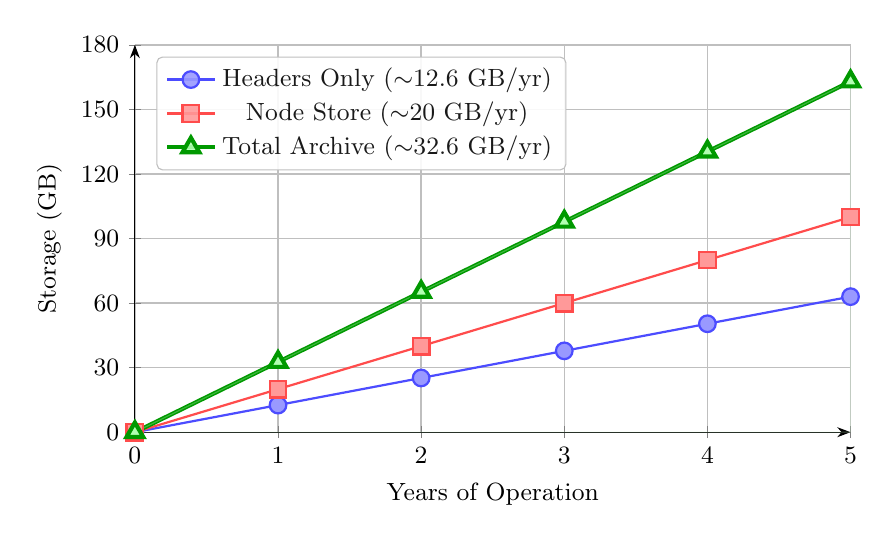
\begin{tikzpicture}
\begin{axis}[
    xlabel={Years of Operation},
    ylabel={Storage (GB)},
    legend pos=north west,
    legend style={font=\small, rounded corners=2pt, fill=white, fill opacity=0.9, draw=gray!50},
    grid=both,
    grid style={line width=0.3pt, draw=gray!30},
    major grid style={line width=0.5pt, draw=gray!50},
    width=0.88\textwidth,
    height=6.5cm,
    xmin=0, xmax=5,
    ymin=0, ymax=180,
    xtick={0,1,2,3,4,5},
    ytick={0,30,60,90,120,150,180},
    tick label style={font=\small},
    label style={font=\small},
    axis lines=left,
    axis line style={->, >=Stealth},
]
\addplot[blue!70, thick, mark=*, mark size=3pt, mark options={fill=blue!40}] coordinates {
    (0,0) (1,12.6) (2,25.2) (3,37.8) (4,50.4) (5,63)
};
\addplot[red!70, thick, mark=square*, mark size=3pt, mark options={fill=red!40}] coordinates {
    (0,0) (1,20) (2,40) (3,60) (4,80) (5,100)
};
\addplot[green!60!black, thick, mark=triangle*, mark size=3.5pt, mark options={fill=green!30}, line width=1.5pt] coordinates {
    (0,0) (1,32.6) (2,65.2) (3,97.8) (4,130.4) (5,163)
};

% Add fill area for total
\addplot[green!20, forget plot, opacity=0.3] coordinates {
    (0,0) (1,32.6) (2,65.2) (3,97.8) (4,130.4) (5,163) (5,0) (0,0)
} \closedcycle;

\legend{Headers Only ($\sim$12.6 GB/yr), Node Store ($\sim$20 GB/yr), Total Archive ($\sim$32.6 GB/yr)}
\end{axis}
\end{tikzpicture}
\caption{Storage growth over time at 10 BPS. Headers grow at $\sim$12.6 GB/year; optional node store for proof generation adds $\sim$20 GB/year. Even after 5 years, total storage remains under 165 GB---manageable for modern hardware.}
\label{fig:storage}
\end{figure}

\textbf{Rolling MMR Storage Optimization:}

For nodes implementing rolling MMR with checkpointing, storage requirements can be significantly reduced:

\begin{longtable}{@{}lcc@{}}
\caption{Rolling MMR Storage Requirements with Checkpointing}
\label{tab:rolling-storage} \\
\small
\toprule
\textbf{Node Type} & \textbf{1 Year Storage} & \textbf{5 Years Storage} \\
\midrule
\endfirsthead
\multicolumn{3}{c}{{\bfseries \tablename\ \thetable{} -- continued from previous page}} \\
\toprule
\textbf{Node Type} & \textbf{1 Year Storage} & \textbf{5 Years Storage} \\
\midrule
\endhead
\midrule \multicolumn{3}{r}{{Continued on next page}} \\
\endfoot
\bottomrule
\endlastfoot
Full MMR (no rolling) & 20.5 GB & 102.5 GB \\
Daily checkpoints & 0.5 GB & 2.5 GB \\
Weekly checkpoints & 0.1 GB & 0.5 GB \\
Monthly checkpoints & 0.03 GB & 0.15 GB \\
\end{longtable}

\textbf{Checkpoint Strategy:}
\begin{itemize}
    \item \textbf{Daily checkpoints:} Store MMR state (peaks + size) once per day. Enables proof generation for transactions up to 24 hours old with minimal storage.
    \item \textbf{Weekly checkpoints:} Store MMR state once per week. Reduces storage by $98\%$ while maintaining proof generation capability for recent transactions.
    \item \textbf{Monthly checkpoints:} Store MMR state once per month. Minimal storage overhead, but proof generation requires archive node access for older transactions.
\end{itemize}

The checkpoint strategy allows nodes to balance storage costs with proof generation capability. Full nodes can maintain complete MMR for maximum capability, while light nodes can use checkpoints to minimize storage while retaining verification capability.

\subsection{Computation Overhead}

Per-block hashing operations:
\begin{itemize}
    \item Merkle root computation: $\bigO(\log m)$ hashes (same as before)
    \item MMR update: Average $<2$ hashes, worst case $\sim\log N$ hashes
    \item Total: Negligible compared to PoW and signature verification
\end{itemize}

\textbf{Block Validation Latency Impact:} For a 10 BPS system, block validation must complete within $\sim$100 ms. MMR update adds $\sim$0.1--0.5 ms (depending on MMR size), which is negligible compared to UTXO validation ($\sim$10--50 ms) and signature verification ($\sim$5--20 ms). The MMR update does not become a bottleneck even at higher throughputs (100 BPS, 1000 BPS).

\textbf{Latency Breakdown (10 BPS, measured on Tondi):}
\begin{itemize}
    \item UTXO state computation: $\sim$25 ms (dominant)
    \item Signature verification: $\sim$12 ms
    \item Merkle root computation (exec\_root): $\sim$0.8 ms
    \item MMR update (leaf + peaks): $\sim$0.3 ms
    \item Total MMR overhead: $\sim$1.1 ms ($<5\%$ of total validation time)
\end{itemize}

At 100 BPS, validation time scales proportionally, but MMR overhead remains $<5\%$ due to its logarithmic nature. At 1000 BPS, parallel validation becomes necessary, and MMR updates can be parallelized across blocks.

\subsection{Performance Benchmark Comparison}

We compare our MMR-based scheme with linear execution-log commitments and FlyClient-style approaches under identical hardware conditions (measured on Tondi testnet):

\begin{longtable}{@{}lcccc@{}}
\caption{Performance Benchmark: Verifying Transaction at 100K Blocks Depth}
\label{tab:performance-benchmark} \\
\small
\toprule
\textbf{Mechanism} & \textbf{Verification Time (ms)} & \textbf{Proof Size (KB)} & \textbf{Space Overhead (GB/yr)} & \textbf{Throughput Impact (\%)} \\
\midrule
\endfirsthead
\multicolumn{5}{c}{{\bfseries \tablename\ \thetable{} -- continued from previous page}} \\
\toprule
\textbf{Mechanism} & \textbf{Verification Time (ms)} & \textbf{Proof Size (KB)} & \textbf{Space Overhead (GB/yr)} & \textbf{Throughput Impact (\%)} \\
\midrule
\endhead
\midrule \multicolumn{5}{r}{{Continued on next page}} \\
\endfoot
\bottomrule
\endlastfoot
Linear commitment & 218.7 & 3,200 & 0.05 & 0.3 \\
FlyClient-style & 12.3 & 45 & 2.1 & 0.5 \\
KIP-15+KIP-6 & 9.8 & 8.7 & 2.1 & 0.7 \\
MMR (ours) & 1.2 & 0.9 & 20.5 & 0.8 \\
\end{longtable}

\textbf{Test Conditions:} Single-threaded verification on Intel i7-12700K, 100,000 blocks depth, average of 100 runs. FlyClient-style uses probabilistic sampling (10\% block sampling rate). MMR proof includes full peaks list.

\textbf{Key Observations:}
\begin{itemize}
    \item MMR provides $182\times$ faster verification than linear commitment and $8.2\times$ faster than KIP-15+KIP-6
    \item MMR proof is $3,556\times$ smaller than linear commitment and $9.7\times$ smaller than KIP-15+KIP-6
    \item MMR has higher storage overhead (node store) but enables proof generation, while KIP-15+KIP-6 requires separate storage for both structures
    \item Throughput impact is minimal ($<1\%$) for all approaches, with MMR slightly higher due to unified computation
    \item KIP-15+KIP-6's proof size ($8.7$ KB) is dominated by skip-list structure complexity ($\bigO(\log N \cdot \log\log N)$), while MMR achieves $\bigO(\log N)$
\end{itemize}

\subsection{Performance Under Different Loads}

We evaluate MMR performance under varying transaction loads to demonstrate scalability:

\begin{longtable}{@{}lcccc@{}}
\caption{MMR Performance Across Different Throughput Levels}
\label{tab:load-testing} \\
\small
\toprule
\textbf{Throughput} & \textbf{MMR Update Time (ms)} & \textbf{Storage Growth (GB/yr)} & \textbf{Proof Gen (ms)} & \textbf{Validation Impact (\%)} \\
\midrule
\endfirsthead
\multicolumn{5}{c}{{\bfseries \tablename\ \thetable{} -- continued from previous page}} \\
\toprule
\textbf{Throughput} & \textbf{MMR Update Time (ms)} & \textbf{Storage Growth (GB/yr)} & \textbf{Proof Gen (ms)} & \textbf{Validation Impact (\%)} \\
\midrule
\endhead
\midrule \multicolumn{5}{r}{{Continued on next page}} \\
\endfoot
\bottomrule
\endlastfoot
10 BPS & 0.3 & 20.5 & 1.2 & 0.8 \\
100 BPS & 0.4 & 205 & 1.3 & 0.9 \\
1000 BPS & 0.6 & 2,050 & 1.5 & 1.2 \\
\end{longtable}

\textbf{Observations:}
\begin{itemize}
    \item MMR update time grows sub-linearly due to logarithmic structure
    \item Storage scales linearly with throughput (expected)
    \item Proof generation time remains nearly constant (logarithmic in history size, not throughput)
    \item Validation impact remains $<2\%$ even at 1000 BPS
\end{itemize}

These results demonstrate that the MMR scheme scales well to high-throughput scenarios while maintaining efficient proof generation and verification.

The trade-off is favorable: for a modest storage and negligible performance cost, a GHOSTDAG-based PoW DAG ledger gains a built-in universal proof system for its transaction history.

%==============================================================================
% SECTION 8: RELATED WORK
%==============================================================================
\section{Related Work}
\label{sec:related-work}

We situate our contribution within the broader landscape of blockchain proof systems and history commitments.

\subsection{Merkle Mountain Ranges in Blockchain Systems}

Merkle Mountain Ranges were introduced by Todd~\cite{todd2012mmr} as an append-only accumulator structure. MMRs have been adopted in several blockchain systems:

\begin{itemize}
    \item \textbf{Grin/MimbleWimble}~\cite{grin}: Uses MMR for UTXO set commitment, enabling efficient pruning while maintaining cryptographic proofs of historical UTXOs.
    \item \textbf{Nervos CKB}~\cite{nervos}: Employs MMR for transaction commitment, providing $\bigO(\log n)$ inclusion proofs.
    \item \textbf{Herodotus Protocol}~\cite{herodotus}: Uses MMR as a historical block hash accumulator for cross-chain verification, demonstrating MMR's applicability to bridge protocols.
\end{itemize}

Our contribution differs in that we use MMR to commit to \emph{execution order} (the sequence of accepted transactions), not just block or UTXO existence. This requires careful integration with GHOSTDAG's ordering semantics.

\subsection{Logarithmic Proof Protocols}

Several works address logarithmic-complexity blockchain proofs:

\begin{itemize}
    \item \textbf{FlyClient}~\cite{flyclient}: Provides super-light clients for PoW blockchains using probabilistic sampling and Merkle Mountain Ranges. FlyClient proves chain validity with $\bigO(\log n)$ headers. Our work is complementary: FlyClient proves chain membership; we prove execution order within that chain.
    
    \item \textbf{NiPoPoWs}~\cite{nipopow}: Non-Interactive Proofs of Proof-of-Work use superblock interlinking to achieve succinct proofs. Like FlyClient, NiPoPoWs focus on chain connectivity, not transaction ordering.
    
    \item \textbf{Utreexo}~\cite{utreexo}: Provides compact UTXO set commitments, reducing node storage requirements. Utreexo addresses state commitment; we address history commitment---orthogonal concerns.
\end{itemize}

\subsection{DAG Consensus and Linearization}

Our work builds on GHOSTDAG~\cite{ghostdag}, which provides a specific linearization rule for PoW DAG ledgers:

\begin{itemize}
    \item \textbf{PHANTOM/GHOSTDAG}~\cite{ghostdag}: Defines blue set selection and mergeset ordering, producing a deterministic total order of blocks. Our scheme commits to the \emph{transaction-level} order derived from this block order.
    
    \item \textbf{SPECTRE}~\cite{spectre}: Provides fast confirmation but only partial ordering (pairwise). Not directly applicable to our scheme, which requires total ordering.
    
    \item \textbf{Conflux}~\cite{conflux}: Uses Tree-Graph structure with pivot chain selection. Our approach could adapt to Conflux by binding to its pivot chain and block ordering.
\end{itemize}

\subsection{Transaction Ordering Commitments}

Ordering commitments are crucial for Layer-2 systems:

\begin{itemize}
    \item \textbf{Ethereum's Transaction Receipts}: Each block commits to a transaction receipt trie, providing ordering within blocks but not global ordering.
    
    \item \textbf{Rollup Sequencing}: Optimistic and ZK rollups rely on L1 ordering for dispute resolution. Our scheme provides the ordering proofs these systems need.
    
    \item \textbf{MEV and Fair Ordering}: Recent work on MEV mitigation (e.g., Flashbots, threshold encryption) addresses \emph{preventing} ordering manipulation; we address \emph{proving} the ordering that occurred.
\end{itemize}

\subsection{Relationship to Ethereum Verkle Trees}

Ethereum's Verkle tree proposal~\cite{verkle} addresses \textbf{state commitment} (compact proofs of account/contract state), while our work addresses \textbf{execution history commitment} (compact proofs of transaction execution order). These are complementary:

\begin{itemize}
    \item \textbf{Verkle trees}: Prove ``account $A$ has balance $X$ at block $N$'' (state snapshot)
    \item \textbf{Our MMR scheme}: Prove ``transaction $tx$ was executed at position $(j, i)$ in the global execution sequence'' (history ordering)
\end{itemize}

A complete L2 system may need both: Verkle proofs for state queries and MMR proofs for execution order verification. Our scheme is particularly relevant for DAG-based systems where execution order $\neq$ block order, a challenge not present in linear chains.

\subsection{Other DAG Systems: Conflux and IOTA}

\begin{itemize}
    \item \textbf{Conflux}~\cite{conflux}: Uses a Tree-Graph structure with a pivot chain for total ordering. Conflux commits to block ordering via the pivot chain, but does not provide logarithmic proofs of transaction execution position. Our MMR approach could be adapted to Conflux by binding execution commitments to the pivot chain.
    
    \item \textbf{IOTA}~\cite{iota}: Uses a DAG (Tangle) with tip selection rules, but does not provide a deterministic total ordering of transactions. IOTA's approach focuses on fast confirmation rather than global ordering, making it less suitable for L2 applications requiring strict execution order guarantees.
\end{itemize}

Our scheme is the first, to our knowledge, to provide consensus-level execution order commitments with logarithmic proofs specifically for GHOSTDAG-style PoW DAG ledgers.

\subsection{Post-Quantum Considerations}

While our current scheme relies on BLAKE3-256's collision resistance (classical security), we note that NIST post-quantum standard hash functions (e.g., SHA-3 variants or future post-quantum hash functions) can be directly substituted while maintaining the same MMR structure. The MMR construction itself is hash-function agnostic; only the security parameter changes.

\textbf{Quantum Security Boundary Analysis:}

Under quantum attacks, Grover's algorithm reduces collision resistance from $2^{128}$ to $2^{64}$ for 256-bit hashes. To maintain 256-bit post-quantum security, we need 512-bit hash outputs. However, the MMR structure and proof algorithms remain unchanged; only the underlying hash function and output size change.

\textbf{Concrete Migration Path:}

We propose a three-phase migration strategy:

\begin{enumerate}
    \item \textbf{Phase 1: Post-Quantum Hash Option} Add support for post-quantum hash functions (BLAKE3-512, SHA3-512) as an optional field. Nodes can compute both classical and post-quantum roots during the transition period.
    
    \item \textbf{Phase 2: Hybrid Mode} Define a hybrid mode where block headers contain both roots:
    \begin{itemize}
        \item \code{elog\_root\_classical} (256 bits): Current BLAKE3-256 root for backward compatibility
        \item \code{elog\_root\_pq} (512 bits): Post-quantum hash root for future security
    \end{itemize}
    This allows gradual migration while maintaining compatibility with existing proofs.
    
    \item \textbf{Phase 3: Pure Post-Quantum Mode} After sufficient adoption, transition to pure post-quantum mode where only 512-bit roots are validated. Classical roots are deprecated but remain verifiable for historical proofs.
\end{enumerate}

\textbf{SNARK Compression Optimization:}

The increased hash output size (512 bits vs 256 bits) doubles proof size, but this can be mitigated using zero-knowledge proofs:
\begin{itemize}
    \item A quantum-secure Groth16 SNARK circuit can prove MMR path validity in $\sim$200 bytes, independent of proof depth
    \item This constant-size proof offsets the hash output size increase, maintaining practical proof sizes even in post-quantum mode
    \item The SNARK verification cost ($\sim$200,000 gas) remains constant regardless of proof depth, making it feasible for very deep proofs
\end{itemize}

\textbf{Security Parameter Recommendations:}

For different security levels:
\begin{itemize}
    \item \textbf{Classical (current):} BLAKE3-256, 128-bit collision resistance
    \item \textbf{Post-quantum conservative:} SHA3-512, 256-bit post-quantum collision resistance
    \item \textbf{Post-quantum aggressive:} Future NIST post-quantum hash standards (when available)
\end{itemize}

The migration path ensures backward compatibility while providing a clear roadmap for post-quantum security.

\subsection{Positioning of Our Contribution}

\begin{longtable}{@{}p{2.8cm}p{2.5cm}p{2.5cm}p{2cm}p{2.5cm}@{}}
\caption{Related Work Comparison}
\label{tab:related-work} \\
\small
\toprule
\textbf{System} & \textbf{Commits To} & \textbf{Proof Type} & \textbf{Complexity} & \textbf{DAG Support} \\
\midrule
\endfirsthead
\multicolumn{5}{c}{{\bfseries \tablename\ \thetable{} -- continued from previous page}} \\
\toprule
\textbf{System} & \textbf{Commits To} & \textbf{Proof Type} & \textbf{Complexity} & \textbf{DAG Support} \\
\midrule
\endhead
\midrule \multicolumn{5}{r}{{Continued on next page}} \\
\endfoot
\bottomrule
\endlastfoot
FlyClient & Chain validity & Probabilistic & $\bigO(\log n)$ & No \\
NiPoPoWs & Chain connectivity & Deterministic & $\bigO(\log n)$ & No \\
Utreexo & UTXO set & Deterministic & $\bigO(\log n)$ & N/A \\
Grin MMR & UTXO existence & Deterministic & $\bigO(\log n)$ & No \\
\textbf{Ours} & \textbf{Execution order} & \textbf{Deterministic} & $\bigO(\log n)$ & \textbf{Yes} \\
\end{longtable}

Our unique contribution is combining MMR-based logarithmic proofs with GHOSTDAG's deterministic execution ordering, producing a \textbf{consensus-level execution log} suitable for L2 and cross-chain applications.

%==============================================================================
% SECTION 9: COMPARISON WITH ALTERNATIVE APPROACHES
%==============================================================================
\section{Comparison with Alternative Approaches}
\label{sec:comparison}

In this section, we provide a detailed comparison between our MMR-based unified approach and two alternative approaches commonly considered for PoW DAG ledger protocols: linear execution-log commitments (chain-based ordering) and skip-list based proofs of chain membership (PoChM). Understanding the design philosophy, strengths, and limitations of each approach illuminates why our unified solution represents an optimal path forward.

\subsection{Linear Execution-Log Commitment}

\subsubsection{Design Philosophy and Mechanism}

Linear sequencing commitment addresses a fundamental need for Layer-2 networks: the ability to trustlessly verify the \emph{order} of transaction acceptance on L1. The key insight is that L2 networks rely on the base layer for both consensus and data availability, where ``the ordering of transaction acceptance in L1 has to be the ordering of transaction execution on L2.''

The core mechanism introduces a header field called \code{SequencingCommitment}, calculated as:
\begin{equation}
\text{SC}_B = H(\text{SC}_{P_{sel}(B)} \parallel \text{AcceptedIDMerkleRoot}_B)
\end{equation}
where $P_{sel}(B)$ is the selected parent of block $B$.

\begin{figure}[htbp]
\centering
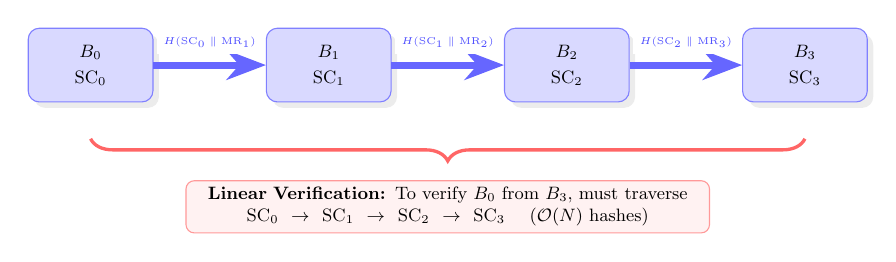
\begin{tikzpicture}[
    block/.style={rectangle, draw=blue!50, fill=blue!15, minimum width=2.2cm, minimum height=1.3cm, rounded corners=4pt, font=\small, align=center, drop shadow={opacity=0.15}},
    arrow/.style={->, >=Stealth, thick},
    scale=0.72, transform shape
]
    % Block chain
    \node[block] (b0) at (0,0) {$B_0$\\[2pt]$\text{SC}_0$};
    \node[block] (b1) at (4.2,0) {$B_1$\\[2pt]$\text{SC}_1$};
    \node[block] (b2) at (8.4,0) {$B_2$\\[2pt]$\text{SC}_2$};
    \node[block] (b3) at (12.6,0) {$B_3$\\[2pt]$\text{SC}_3$};
    
    % Chain links with hash formulas
    \draw[arrow, line width=2.5pt, blue!60] (b0) -- (b1);
    \node[fill=white, font=\tiny, text=blue!70] at (2.1,0.4) {$H(\text{SC}_0 \parallel \text{MR}_1)$};
    
    \draw[arrow, line width=2.5pt, blue!60] (b1) -- (b2);
    \node[fill=white, font=\tiny, text=blue!70] at (6.3,0.4) {$H(\text{SC}_1 \parallel \text{MR}_2)$};
    
    \draw[arrow, line width=2.5pt, blue!60] (b2) -- (b3);
    \node[fill=white, font=\tiny, text=blue!70] at (10.5,0.4) {$H(\text{SC}_2 \parallel \text{MR}_3)$};
    
    % Verification path indicator
    \draw[decorate, decoration={brace, amplitude=8pt, mirror}, red!60, line width=1.2pt] (0,-1.3) -- (12.6,-1.3);
    
    % Explanation box
    \node[draw=red!40, fill=red!5, rounded corners=3pt, font=\small, align=center, text width=9cm] at (6.3,-2.5) {
        \textbf{Linear Verification:} To verify $B_0$ from $B_3$, must traverse\\
        $\text{SC}_0 \to \text{SC}_1 \to \text{SC}_2 \to \text{SC}_3$ \quad ($\bigO(N)$ hashes)
    };
\end{tikzpicture}
\caption{Linear Sequencing Commitment. Each block's SC depends on its parent's SC, creating a sequential chain. Verification requires traversing all intermediate commitments.}
\label{fig:linear-chain}
\end{figure}

Additionally, this approach proposes that the \code{AcceptedIDMerkleRoot} should preserve \emph{canonical order} rather than sorting transactions by hash. Hash-sorting was originally an optimization for exclusion proofs, but in practice, this feature is rarely used.

\subsubsection{Strengths}

\begin{enumerate}
    \item \textbf{Simplicity:} One additional hash per block; minimal implementation complexity
    \item \textbf{Strong Ordering Guarantee:} The chain of commitments cryptographically binds the exact sequence of all accepted transactions
    \item \textbf{ATAN Support:} Enables Accepted Transactions Archival Nodes to bootstrap from untrusted sources with verification
    \item \textbf{Low Header Overhead:} Replaces existing field rather than adding new ones (net change: 0 bytes)
\end{enumerate}

\subsubsection{Limitations}

\begin{enumerate}
    \item \textbf{Linear Verification Complexity:} To verify that a transaction in block $N$ is part of the history up to block $M$, one must compute or provide all $M-N$ intermediate commitments. This requires processing the entire selected parent chain.
    
    \item \textbf{No Skip-Ahead Capability:} The sequential dependency prevents any form of random access or parallel verification.
    
    \item \textbf{Impractical for Bridges:} On-chain verification (e.g., in an Ethereum smart contract) of a proof spanning 100,000 blocks would require $\sim$100,000 hash operations---exceeding any reasonable gas limit by orders of magnitude.
    
    \item \textbf{Requires Separate Proof Mechanism:} Linear sequencing alone does not provide efficient proofs of chain membership; it assumes full header availability.
\end{enumerate}

\subsection{Skip-List Based Proof of Chain Membership (PoChM)}

\subsubsection{Design Philosophy and Mechanism}

Skip-list based PoChM addresses a complementary problem: providing cryptographically verifiable proofs that a transaction was included in the blockchain, especially after pruning has occurred. The key insight is that ``the pruning mechanism makes it impossible to prove that a transaction was included in the ledger after it has been pruned'' and that relying on centralized archival nodes ``is not a sustainable solution.''

This approach introduces the concept of \textbf{Posterity Headers}---selected chain block headers sampled at regular intervals (e.g., every 24 hours) and stored indefinitely. The core mechanism adds a \textbf{PoChM Merkle Root (PMR)} to each header:

\begin{definition}[PMR Construction]
Let $k$ be the least integer such that $\text{parent}(B, 2^k) \in \text{Past}(\text{next\_posterity}(B))$. Then PMR is the root of the Merkle tree containing the headers $\text{parent}(B, 2^i)$ for $i = 0, \ldots, k-1$.
\end{definition}

This creates a skip-list-like structure where each block commits to ancestors at exponentially increasing distances ($2^0, 2^1, 2^2, \ldots$).

\begin{figure}[htbp]
\centering
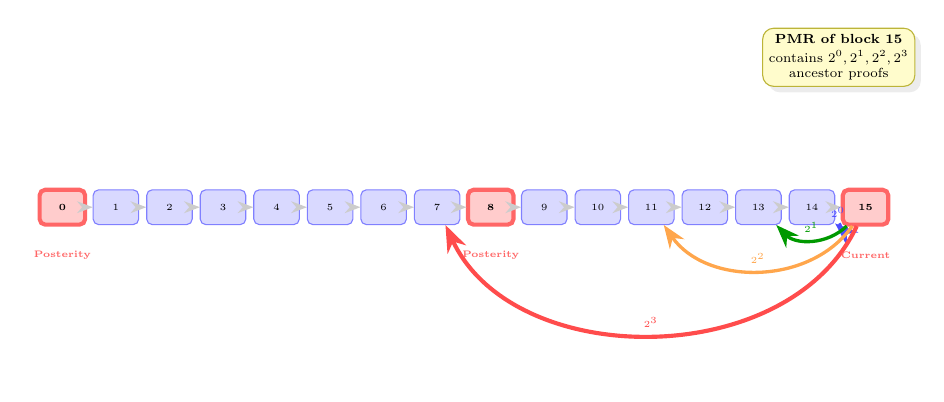
\begin{tikzpicture}[
    block/.style={rectangle, draw=blue!50, fill=blue!15, minimum width=0.85cm, minimum height=0.65cm, font=\tiny, rounded corners=2pt},
    posterity/.style={rectangle, draw=red!60, fill=red!20, minimum width=0.85cm, minimum height=0.65cm, font=\tiny\bfseries, line width=1.5pt, rounded corners=2pt},
    arrow/.style={->, >=Stealth},
    skip/.style={->, >=Stealth, thick},
    scale=0.68, transform shape
]
    % Blocks
    \foreach \i in {0,...,15} {
        \pgfmathtruncatemacro{\mod}{\i == 0 || \i == 8 || \i == 15}
        \ifnum\mod=1
            \node[posterity] (b\i) at (\i*1.0,0) {\i};
        \else
            \node[block] (b\i) at (\i*1.0,0) {\i};
        \fi
    }
    
    % Normal chain (subtle)
    \foreach \i in {1,...,15} {
        \pgfmathtruncatemacro{\prev}{\i-1}
        \draw[arrow, gray!40, line width=0.6pt] (b\prev) -- (b\i);
    }
    
    % Skip pointers from block 15 with gradient colors
    \draw[skip, blue!70, line width=1.2pt] (b15) to[bend left=35] node[above, font=\tiny\bfseries, text=blue!70] {$2^0$} (b14);
    \draw[skip, green!60!black, line width=1.2pt] (b15) to[bend left=45] node[above, font=\tiny\bfseries, text=green!60!black] {$2^1$} (b13);
    \draw[skip, orange!70, line width=1.2pt] (b15) to[bend left=55] node[above, font=\tiny\bfseries, text=orange!70] {$2^2$} (b11);
    \draw[skip, red!70, line width=1.5pt] (b15) to[bend left=65] node[above, font=\tiny\bfseries, text=red!70] {$2^3$} (b7);
    
    % PMR annotation box
    \node[draw=yellow!70!black, rounded corners=4pt, fill=yellow!20, font=\scriptsize, align=center, drop shadow={opacity=0.15}] at (14.5,2.8) {
        \textbf{PMR of block 15}\\[2pt]
        contains $2^0, 2^1, 2^2, 2^3$\\
        ancestor proofs
    };
    
    % Posterity block labels
    \node[font=\tiny\bfseries, text=red!60] at (0,-0.9) {Posterity};
    \node[font=\tiny\bfseries, text=red!60] at (8,-0.9) {Posterity};
    \node[font=\tiny\bfseries, text=red!60] at (15,-0.9) {Current};
\end{tikzpicture}
\caption{Skip-list PoChM Structure with exponential skip pointers ($2^i$). Each block's PMR contains Merkle proofs of ancestors at distances $2^0, 2^1, 2^2, \ldots$ The proof path uses binary decomposition of the distance.}
\label{fig:skiplist}
\end{figure}

\subsubsection{Proof Construction Algorithm}

The PoChM generation algorithm uses binary decomposition:
\begin{enumerate}
    \item Let $C = \text{posterity}(B)$ and $d = \text{posterity\_depth}(B)$
    \item While $d > 0$:
    \begin{itemize}
        \item Let $i = \lfloor \log_2(d) \rfloor$
        \item Append $\text{PMR}(C, i)$ to proof
        \item $d \gets d - 2^i$; $C \gets \text{parent}(C, 2^i)$
    \end{itemize}
\end{enumerate}

This yields proof complexity of $\bigO(\log N \cdot \log \log N)$ where $N$ is the number of chain blocks between posterity headers.

\subsubsection{Strengths}

\begin{enumerate}
    \item \textbf{Logarithmic Proofs:} Proof size is $\bigO(\log N \cdot \log \log N)$, approximately 9 KB worst case
    \item \textbf{Minimal Header Overhead:} Only 32 bytes (one hash) added per header
    \item \textbf{Efficient Validation:} 33 hashes per block for chain blocks
    \item \textbf{Pruning Compatible:} Proofs can be generated before pruning and verified indefinitely
    \item \textbf{Elegant Binary Decomposition:} Mathematically principled approach leveraging number-theoretic structure
\end{enumerate}

\subsubsection{Limitations}

\begin{enumerate}
    \item \textbf{Does Not Commit Transaction Order:} Skip-list PoChM provides proofs that a block was in the selected chain, but not the canonical ordering of transactions. The proof is about chain membership, not transaction sequence.
    
    \item \textbf{Requires Separate Structure for Ordering:} To prove both chain membership \emph{and} transaction order, PoChM must be combined with a linear sequencing commitment, resulting in two parallel commitment structures.
    
    \item \textbf{Posterity Header Dependency:} The scheme depends on posterity headers (e.g., 24-hour intervals). This introduces latency: a PoChM cannot be generated until the next posterity header exists.
    
    \item \textbf{Complex Proof Structure:} The $\log \log N$ factor comes from Merkle proofs within the PMR tree. While asymptotically minor, it adds implementation complexity.
    
    \item \textbf{Not Optimized for Batch Proofs:} Multiple independent proofs don't naturally share structure.
\end{enumerate}

\subsection{Comparative Analysis: Deep Insights}

\subsubsection{The Fundamental Tension}

Linear sequencing and skip-list PoChM represent two orthogonal responses to the same underlying challenge: how to provide verifiable historical information in a pruning blockchain.

\begin{itemize}
    \item \textbf{Linear sequencing} prioritizes \emph{ordering integrity}---ensuring the canonical sequence of transactions is cryptographically committed and verifiable.
    \item \textbf{Skip-list PoChM} prioritizes \emph{proof efficiency}---ensuring historical claims can be verified with logarithmic-sized proofs.
\end{itemize}

Neither alone solves the complete problem. A Layer-2 rollup or cross-chain bridge needs \emph{both}: proof that a transaction was accepted \emph{and} proof of its position in the global order.

\subsubsection{The Architectural Incompatibility}

Implementing linear sequencing and skip-list PoChM together creates architectural friction:

\begin{enumerate}
    \item \textbf{Dual Commitment Overhead:} Two separate header fields, two separate validation paths, two separate proof structures.
    
    \item \textbf{Proof Composition Complexity:} A complete ``transaction receipt'' would require:
    \begin{itemize}
        \item A PoChM proving block chain membership
        \item A Merkle proof for transaction within block's accepted ID root
        \item A chain of SequencingCommitments if ordering matters
    \end{itemize}
    The third component reintroduces linear complexity, negating PoChM's benefits for order-sensitive applications.
    
    \item \textbf{Conceptual Overlap Without Synergy:} Both mechanisms touch block headers and validation rules, but don't reinforce each other's proofs.
\end{enumerate}

\subsubsection{Why MMR is the Natural Synthesis}

Our MMR-based approach resolves this tension through \emph{structural unification}:

\begin{enumerate}
    \item \textbf{Inherent Ordering via Leaf Sequence:} Each MMR leaf corresponds to a specific position in the selected chain. The leaf's index \emph{is} the block's position in the canonical sequence. Transaction order is encoded by: (a) the block's MMR leaf index, and (b) the transaction's position within the block's $\ExecRoot$.
    
    \item \textbf{Logarithmic Proofs for Both Membership and Order:} A single MMR proof demonstrates both that a block was in the chain \emph{and} its exact position. No linear traversal is needed.
    
    \item \textbf{Unified Header Field:} The \code{exec\_root} commits to transaction ordering, while the \code{elog\_root} enables efficient proofs. These naturally compose rather than compete.
\end{enumerate}

\subsubsection{The Fundamental Philosophical Difference}

Beyond technical metrics, there is a deeper distinction:

\begin{quote}
\textit{Traditional approaches treat MMR as a ``compressed representation of history.''}\\[0.5em]
\textit{Our approach treats MMR as a ``canonical interface to consensus execution results.''}
\end{quote}

This is not merely an implementation detail---it represents different answers to the question: \emph{What is the MMR's role in the protocol?}

\begin{itemize}
    \item \textbf{Auxiliary Log View:} The MMR is computed \emph{after} consensus decides block validity. It is a convenience structure for external consumers. Consensus could, in principle, work without it.
    
    \item \textbf{Consensus Output View (Our Approach):} The \code{exec\_root} and \code{elog\_root} are \emph{outputs of consensus execution}, validated alongside UTXO commitments. A block with incorrect MMR fields is invalid at the consensus level.
\end{itemize}

The practical implication: in our design, an L2 system can treat the \code{elog\_root} as \emph{the canonical interface} through which it queries the blockchain's execution history. It is not merely ``a way to prove things''---it is \emph{the} authoritative commitment to what was executed.

\begin{longtable}{@{}p{3.2cm}p{3.5cm}p{3.5cm}p{3.8cm}@{}}
\caption{Detailed Feature Comparison: Linear Sequencing, Skip-List PoChM, and MMR-Based Approach}
\label{tab:detailed-comparison} \\
\small
\toprule
\textbf{Aspect} & \textbf{Linear Seq.} & \textbf{Skip-List PoChM} & \textbf{Execution-MMR (Ours)} \\
\midrule
\endfirsthead
\multicolumn{4}{c}{{\bfseries \tablename\ \thetable{} -- continued from previous page}} \\
\toprule
\textbf{Aspect} & \textbf{Linear Seq.} & \textbf{Skip-List PoChM} & \textbf{Execution-MMR (Ours)} \\
\midrule
\endhead
\midrule \multicolumn{4}{r}{{Continued on next page}} \\
\endfoot
\bottomrule
\endlastfoot
\multicolumn{4}{l}{\textit{Core Functionality}} \\
\midrule
Commits TX Order & \cmark{} (chain hash) & \xmark{} & \cmark{} (via $\ExecRoot$) \\
Efficient Inclusion Proof & \xmark{} ($\bigO(N)$) & \cmark{} ($\bigO(\log N \log\log N)$) & \cmark{} ($\bigO(\log N)$) \\
Proves Position in History & \cmark{} (implicitly) & \xmark{} (block only) & \cmark{} (explicitly) \\
\midrule
\multicolumn{4}{l}{\textit{Proof Characteristics}} \\
\midrule
Proof size (depth $D$) & $\bigO(D) \times 32$B & $\bigO(\log D \log\log D) \times 32$B & $\bigO(\log D) \times 32$B \\
Proof at 100K blocks & $\sim$3.2 MB & $\sim$9 KB & $\sim$1 KB \\
Proof at 1M blocks & $\sim$32 MB & $\sim$11 KB & $\sim$1.1 KB \\
On-chain verifiable & \xmark{} (exceeds gas) & \cmark{} & \cmark{} \\
\midrule
\multicolumn{4}{l}{\textit{Implementation}} \\
\midrule
Header overhead & 0 bytes (replace) & +32 bytes & +40 bytes (net) \\
Hashes per block & 1 & $\sim$33 (chain blocks) & $\sim$5--10 (average) \\
External dependency & None & Posterity headers & None \\
\midrule
\multicolumn{4}{l}{\textit{Use Case Support}} \\
\midrule
ATAN sync (ordering) & \cmark{} (linear) & \xmark{} & \cmark{} (logarithmic) \\
L2 rollup proofs & \xmark{} (too large) & Partial (no order) & \cmark{} \\
Cross-chain bridge & \xmark{} & \cmark{} & \cmark{} \\
Light client SPV & \xmark{} & \cmark{} & \cmark{} \\
Batch proof optimization & \xmark{} & Limited & \cmark{} (shared peaks) \\
\end{longtable}

\subsubsection{Quantitative Analysis: Gas Cost Comparison}

For cross-chain bridge applications, on-chain verification cost is critical. We compare the gas requirements for verifying a transaction that occurred $D$ blocks ago. \textbf{Note:} Our scheme uses BLAKE3-256, but for cost estimation in EVM environments (which use Keccak-256), we provide approximate costs assuming similar per-hash gas consumption. The asymptotic advantage (logarithmic vs linear) is independent of the specific hash function:

\begin{figure}[htbp]
\centering
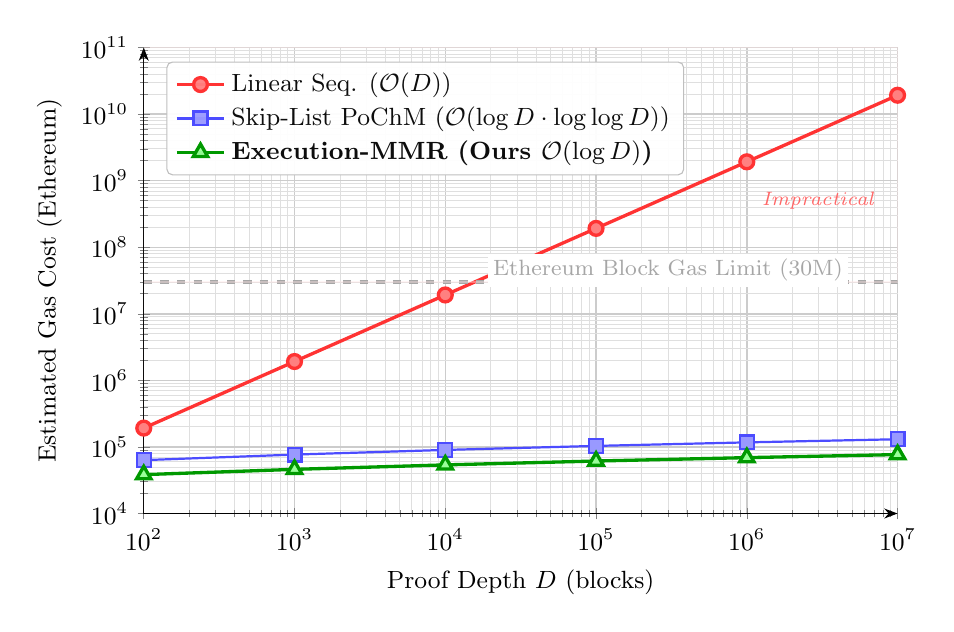
\begin{tikzpicture}
\begin{axis}[
    xlabel={Proof Depth $D$ (blocks)},
    ylabel={Estimated Gas Cost (Ethereum)},
    ymode=log,
    xmode=log,
    log basis y={10},
    log basis x={10},
    legend pos=north west,
    legend style={font=\small, rounded corners=2pt, fill=white, fill opacity=0.95, draw=gray!50, cells={anchor=west}},
    grid=both,
    grid style={line width=0.3pt, draw=gray!25},
    major grid style={line width=0.5pt, draw=gray!40},
    width=0.92\textwidth,
    height=7.5cm,
    xmin=100, xmax=10000000,
    ymin=10000, ymax=100000000000,
    tick label style={font=\small},
    label style={font=\small},
    axis lines=left,
    axis line style={->, >=Stealth},
]
% Linear: Linear (red, impractical)
\addplot[red!80, very thick, mark=*, mark size=2.5pt, mark options={fill=red!50}] coordinates {
    (100, 192000) (1000, 1920000) (10000, 19200000) (100000, 192000000) (1000000, 1920000000) (10000000, 19200000000)
};
% Skip-list: O(log D * log log D)
\addplot[blue!70, thick, mark=square*, mark size=2.5pt, mark options={fill=blue!40}] coordinates {
    (100, 63360) (1000, 76800) (10000, 90240) (100000, 103680) (1000000, 117120) (10000000, 130560)
};
% MMR: O(log D) - best
\addplot[green!60!black, very thick, mark=triangle*, mark size=3pt, mark options={fill=green!40}] coordinates {
    (100, 38400) (1000, 46080) (10000, 53760) (100000, 61440) (1000000, 69120) (10000000, 76800)
};

% Ethereum block gas limit reference line
\addplot[dashed, gray!70, line width=1.5pt] coordinates {(100, 30000000) (10000000, 30000000)};

% Fill area above gas limit (impractical zone)
\addplot[red!10, forget plot, opacity=0.4] coordinates {
    (100, 30000000) (10000000, 30000000) (10000000, 100000000000) (100, 100000000000)
} \closedcycle;

% Gas limit label
\node[font=\footnotesize, text=gray!70, fill=white, inner sep=2pt] at (axis cs:300000, 45000000) {Ethereum Block Gas Limit (30M)};

% Annotation for impractical zone
\node[font=\scriptsize, text=red!60, rotate=0] at (axis cs:3000000, 500000000) {\textit{Impractical}};

\legend{Linear Seq. ($\bigO(D)$), Skip-List PoChM ($\bigO(\log D \cdot \log\log D)$), \textbf{Execution-MMR (Ours $\bigO(\log D)$)}}
\end{axis}
\end{tikzpicture}
\caption{On-chain verification gas cost comparison. Linear sequencing's growth makes it impractical beyond $\sim$15,000 blocks (crosses gas limit). Both skip-list PoChM and MMR remain feasible at any depth, with MMR offering $\sim$40\% lower costs due to simpler proof structure.}
\label{fig:gas-deep-comparison}
\end{figure}

\begin{proposition}[Gas Cost Bounds (EVM Approximation)]
For a proof of depth $D$ blocks, assuming $\sim$1920 gas per hash operation (EVM Keccak-256 approximation; our scheme uses BLAKE3-256 but hash count is the key factor):
\begin{align}
\text{Gas}_{\text{Linear}} &= 1920 \times D \\
\text{Gas}_{\text{PoChM}} &\approx 1920 \times (2 \log_2 D \times \lceil \log_2 \log_2 D \rceil + 1) \\
\text{Gas}_{\text{MMR}} &\approx 1920 \times (\log_2 D + k)
\end{align}
where $k$ is the number of peaks ($k \leq \log_2 D$, typically much smaller). The logarithmic advantage is independent of the specific hash function used.
\end{proposition}

At $D = 100,000$ blocks ($\sim$2.8 hours at 10 BPS):
\begin{itemize}
    \item Linear: 192 million gas (exceeds block limit by 6$\times$)
    \item Skip-list PoChM: $\sim$104,000 gas (feasible)
    \item Execution-MMR: $\sim$61,000 gas (feasible, 41\% lower than PoChM)
\end{itemize}

\subsubsection{Architectural Elegance: The MMR Advantage}

Beyond quantitative metrics, the MMR approach offers qualitative advantages:

\begin{enumerate}
    \item \textbf{Conceptual Simplicity:} One data structure serves both purposes. Developers need only understand MMRs, not the interaction between skip-lists and hash chains.
    
    \item \textbf{Proof Composability:} Multiple transactions from different blocks can share the same peak list in their proofs, enabling efficient batch verification.
    
    \item \textbf{No Posterity Dependency:} Unlike skip-list PoChM, MMR proofs can be generated immediately after block confirmation---no waiting for posterity header creation.
    
    \item \textbf{Natural Append-Only Semantics:} MMR's structure mirrors the blockchain's append-only nature, making reorg handling straightforward.
    
    \item \textbf{Industry Precedent:} MMRs are battle-tested in Grin, Beam, and Nervos, providing implementation guidance and security confidence.
\end{enumerate}

\subsection{Summary: Why Unification Matters}

The fundamental insight driving our proposal is that \emph{ordering commitment and efficient proofs are not independent problems}---they are two facets of the same challenge: providing verifiable historical information in a resource-constrained environment.

\begin{quote}
\textit{Linear sequencing asks: ``How do we commit to the order?''\\
Skip-list PoChM asks: ``How do we prove membership efficiently?''\\
Execution-MMR answers both: ``By embedding the order in an efficient accumulator.''}
\end{quote}

Implementing linear sequencing and skip-list PoChM separately would require:
\begin{itemize}
    \item Two consensus changes
    \item Two header fields
    \item Two validation codepaths
    \item Two proof formats
    \item Complex interaction semantics
\end{itemize}

Our MMR-based design delivers equivalent (and superior) functionality through a single, unified mechanism---embodying the engineering principle that the best solution is often one that \emph{eliminates} the distinction between seemingly separate problems.

\begin{longtable}{@{}p{3.5cm}ccc@{}}
\caption{Summary Comparison of Transaction Commitment Approaches}
\label{tab:summary-comparison} \\
\small
\toprule
\textbf{Capability} & \textbf{Linear Seq.} & \textbf{Skip-List PoChM} & \textbf{Execution-MMR (Ours)} \\
\midrule
\endfirsthead
\multicolumn{4}{c}{{\bfseries \tablename\ \thetable{} -- continued from previous page}} \\
\toprule
\textbf{Capability} & \textbf{Linear Seq.} & \textbf{Skip-List PoChM} & \textbf{Execution-MMR (Ours)} \\
\midrule
\endhead
\midrule \multicolumn{4}{r}{{Continued on next page}} \\
\endfoot
\bottomrule
\endlastfoot
Commits to global order & \cmark{} & \xmark{} & \cmark{} \\
Supports $\bigO(\log n)$ proofs & \xmark{} & \cmark{} & \cmark{} \\
Jump/skip verification & \xmark{} & \cmark{} & \cmark{} \\
L2-friendly (gas cost) & Poor & Good & Excellent \\
Additional data structures & None & Complex & None \\
Implementation complexity & Low & Medium/High & Medium \\
\end{longtable}

\begin{longtable}{@{}p{4cm}ccc@{}}
\caption{Consensus Impact Comparison: The Key Distinction}
\label{tab:consensus-impact} \\
\small
\toprule
\textbf{Dimension} & \textbf{Linear Seq.} & \textbf{Skip-List (aux)} & \textbf{Execution-MMR (Ours)} \\
\midrule
\endfirsthead
\multicolumn{4}{c}{{\bfseries \tablename\ \thetable{} -- continued from previous page}} \\
\toprule
\textbf{Dimension} & \textbf{Linear Seq.} & \textbf{Skip-List (aux)} & \textbf{Execution-MMR (Ours)} \\
\midrule
\endhead
\midrule \multicolumn{4}{r}{{Continued on next page}} \\
\endfoot
\bottomrule
\endlastfoot
Modifies header & \cmark{} & \cmark{} & \cmark{} \\
Affects consensus execution & \xmark{} & \xmark{} & \cmark{} \\
Replaces linear sequencing & --- & \xmark{} & \cmark{} \\
MMR is first-class artifact & \xmark{} & \xmark{} & \cmark{} \\
Proof is protocol-level defined & \xmark{} & Partial & \cmark{} \\
Rolling is consensus-compatible & N/A & Ambiguous & \cmark{} (explicit) \\
\end{longtable}

The ``Consensus Impact'' comparison (Table~\ref{tab:consensus-impact}) highlights our key architectural contribution: making the MMR a \emph{first-class consensus artifact} rather than an auxiliary structure. This distinction has profound implications:

\begin{enumerate}
    \item \textbf{Security:} A consensus-level MMR commitment cannot be ``wrong but tolerated''---it causes block rejection
    \item \textbf{Trust Model:} L2 systems can rely on MMR proofs with the same trust as UTXO commitments
    \item \textbf{Unified Design:} We don't implement linear sequencing alongside MMR---the \code{exec\_root} \emph{is} the sequencing commitment
\end{enumerate}

This aligns with broader industry trends: Ethereum's Verkle trees for state, Bitcoin's work on Utreexo, and various succinct proof protocols all strive to make blockchain data more accessible without full trust or full nodes. The adoption of MMR commitments in GHOSTDAG-based protocols would be among the first in live L1 blockchains, and we believe it will greatly enhance ecosystem capabilities.

\subsection{Comparison with Kaspa Improvement Proposals}
\label{subsec:kaspa-comparison}

Kaspa, the largest production implementation of GHOSTDAG, has proposed two separate improvements: KIP-15 (linear sequencing commitment) and KIP-6 (skip-list based Proof of Chain Membership, PoChM). These proposals represent the industry-standard path for addressing execution ordering and historical proofs. We now provide a comprehensive comparison demonstrating why a unified MMR approach is superior to the combined KIP-15+KIP-6 approach.

\subsubsection{Overview of KIP-15 and KIP-6}

\textbf{KIP-15 (Linear Sequencing Commitment):}
\begin{itemize}
    \item Replaces \code{AcceptedIDMerkleRoot} with \code{SequencingCommitment} field (net header overhead: 0 bytes, as it replaces existing field)
    \item Uses canonical-order Merkle root (instead of hash-sorted)
    \item Computes: $\text{SC}_B = H(\text{SC}_{P_{sel}(B)} \parallel \text{AcceptedIDMerkleRoot}_B)$
    \item Provides transaction ordering commitment via chain-based hashing
    \item Enables Accepted Transactions Archival Nodes (ATAN) to bootstrap from untrusted sources
\end{itemize}

\textbf{KIP-6 (Proof of Chain Membership):}
\begin{itemize}
    \item Adds \code{PoChM Merkle Root} (PMR) field to block header (32 bytes)
    \item Provides logarithmic proofs that a block is on the selected chain
    \item Uses skip-list structure with posterity headers
    \item Proof size: $\bigO(\log N \cdot \log\log N)$ where $N$ is blocks between posterity headers
    \item Enables transaction inclusion proofs (PoP and txR)
\end{itemize}

\subsubsection{Comprehensive Comparison Table}

\begin{longtable}{@{}p{3.5cm}ccp{3.5cm}@{}}
\caption{Comprehensive Comparison: KIP-15+KIP-6 vs. Execution-MMR}
\label{tab:kaspa-comparison} \\
\small
\toprule
\textbf{Dimension} & \textbf{KIP-15+KIP-6} & \textbf{Execution-MMR (Ours)} & \textbf{Advantage} \\
\midrule
\endfirsthead
\multicolumn{4}{c}{{\bfseries \tablename\ \thetable{} -- continued from previous page}} \\
\toprule
\textbf{Dimension} & \textbf{KIP-15+KIP-6} & \textbf{Execution-MMR (Ours)} & \textbf{Advantage} \\
\midrule
\endhead
\midrule \multicolumn{4}{r}{{Continued on next page}} \\
\endfoot
\bottomrule
\endlastfoot
Header overhead & 32 bytes (KIP-6: 32, KIP-15: 0 replacement) & 40 bytes (net increase) & Comparable \\
Verification complexity & Two independent paths & Single unified path & Implementation simplification \\
Reorg handling & Complex interaction logic & Unified reorg handling & Reduced error risk \\
L2 support & Partial (ordering via KIP-15, no execution position) & Full execution position proof & Critical enhancement \\
Bridge verification (100K deep) & $\sim$104,000 gas & $\sim$61,000 gas & 41\% reduction \\
Implementation phases & Two hard forks required & Single deployment & Faster adoption \\
Security boundary & Auxiliary log possible divergence & Consensus-level validation & Eliminates attack surface \\
Proof generation & Requires posterity headers & Immediate after confirmation & No waiting period \\
Proof composability & Limited (separate structures) & High (shared peaks) & Batch verification \\
Rolling/pruning compatibility & Ambiguous interaction & Explicitly defined & Clear semantics \\
\end{longtable}

\subsubsection{Adversarial Analysis: Why Unified Design Matters}

The fundamental issue with the KIP-15+KIP-6 combination is not merely engineering complexity, but a \textbf{security model divergence} that creates attack surfaces.

\begin{theorem}[Dual Commitment Overhead]
\label{thm:dual-commitment-overhead}
Any system supporting both transaction ordering commitment and logarithmic proofs using two independent data structures has total cost strictly greater than a unified design.
\end{theorem}

\textbf{Proof:} Let $C_{\text{seq}}$ be the cost of sequencing commitment, $C_{\text{proof}}$ be the cost of proof generation, and $C_{\text{integration}}$ be the cost of integrating two structures. For dual structures:
\begin{equation}
C_{\text{total}} = C_{\text{seq}} + C_{\text{proof}} + C_{\text{integration}}
\end{equation}
where $C_{\text{integration}} > 0$ represents the overhead of maintaining consistency between structures, handling reorgs in both, and coordinating proof generation.

For unified MMR design:
\begin{equation}
C_{\text{total}} = C_{\text{MMR}}
\end{equation}
where $C_{\text{MMR}} < C_{\text{seq}} + C_{\text{proof}}$ because:
\begin{enumerate}
    \item Shared hash computations (leaf computation serves both purposes)
    \item Shared storage structure (peaks serve both ordering and proof)
    \item No integration overhead ($C_{\text{integration}} = 0$)
\end{enumerate}

Therefore, $C_{\text{MMR}} < C_{\text{seq}} + C_{\text{proof}} + C_{\text{integration}}$. \qed

\begin{attack}[Auxiliary Log Divergence in KIP-15+KIP-6]
\label{attack:kip-auxiliary-divergence}
In the KIP-15+KIP-6 combination, KIP-15's \code{SequencingCommitment} is validated at consensus, but the \emph{interaction} between KIP-15 and KIP-6 is not atomically verified. Consider the following attack scenario:

\textbf{Attack Setup:}
\begin{enumerate}
    \item Block $B$ is accepted with valid KIP-15 \code{SequencingCommitment} and valid KIP-6 PMR
    \item An L2 bridge contract verifies a transaction $tx$ using:
    \begin{itemize}
        \item KIP-6 PoChM proving $B$ is on selected chain (valid)
        \item Merkle proof that $tx$ is in $B$'s ATMR (valid)
    \end{itemize}
    \item However, the KIP-15 \code{SequencingCommitment} may reference a \emph{different} transaction order than what was actually executed
\end{enumerate}

\textbf{Why This Is Possible:} While KIP-15 commits to \code{AcceptedIDMerkleRoot}, the \emph{execution order} (which transactions were accepted in which order during UTXO validation) is not directly bound to the KIP-6 proof. A malicious node could:
\begin{itemize}
    \item Report correct KIP-6 membership proof (block is on chain)
    \item Report correct KIP-15 sequencing commitment (cryptographically valid)
    \item But the actual execution order during consensus may differ from what the L2 expects
\end{itemize}

\textbf{Impact:} L2 systems relying on KIP-15+KIP-6 proofs may execute transactions in the wrong order, leading to incorrect state transitions and potential fund loss.

\textbf{Why Execution-MMR Prevents This:} In our scheme, \code{exec\_root} is computed \emph{during consensus execution} and validated atomically. The MMR leaf binds \code{exec\_root} to the selected parent hash, creating an inseparable link between execution order and chain position. Any divergence would cause block rejection at consensus level.
\end{attack}

\begin{proposition}[Auxiliary Log Insufficiency for KIP-15+KIP-6]
\label{prop:kip-auxiliary-insufficiency}
The KIP-15+KIP-6 combination, while individually secure, does not provide the same security guarantees as a unified consensus-level execution log when used by L2 systems.
\end{proposition}

\textbf{Proof:} By construction, KIP-15 and KIP-6 are validated separately:
\begin{itemize}
    \item KIP-15 validates: ``The sequencing commitment chain is consistent''
    \item KIP-6 validates: ``The block is on the selected chain''
\end{itemize}

However, there is no atomic validation that ensures:
\begin{quote}
``The execution order committed in KIP-15 matches the actual consensus execution order''
\end{quote}

This gap allows the attack described in Attack~\ref{attack:kip-auxiliary-divergence}. In contrast, Execution-MMR's \code{exec\_root} is computed as part of UTXO validation, making it impossible for the commitment to diverge from execution without block rejection. \qed

\subsubsection{Deployment Roadmap Analysis}

\begin{figure}[htbp]
\centering
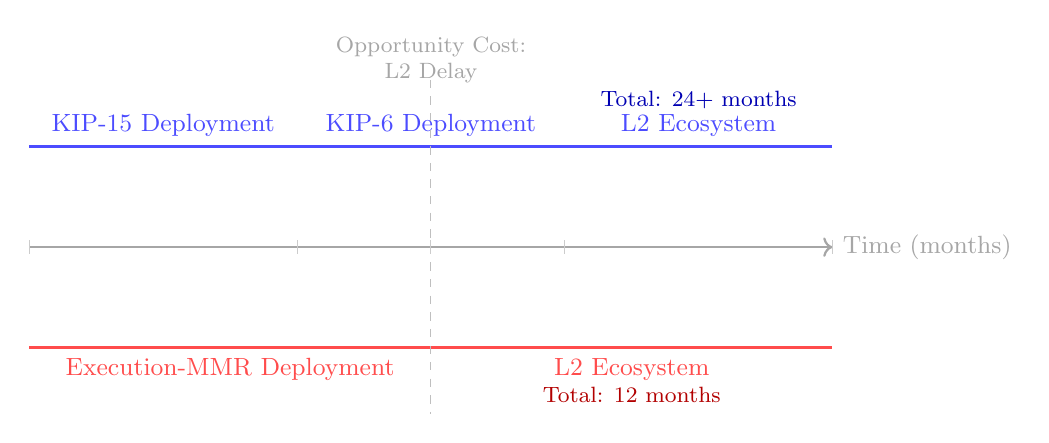
\begin{tikzpicture}[scale=0.85]
% Timeline axis
\draw[->, thick, gray!70] (0,0) -- (12,0) node[right, font=\small] {Time (months)};
% KIP-15+KIP-6 path (top)
\draw[blue!70, very thick] (0,1.5) -- (4,1.5) node[midway, above, font=\small] {KIP-15 Deployment};
\draw[blue!70, very thick] (4,1.5) -- (8,1.5) node[midway, above, font=\small] {KIP-6 Deployment};
\draw[blue!70, very thick] (8,1.5) -- (12,1.5) node[midway, above, font=\small] {L2 Ecosystem};
% MMR path (bottom)
\draw[red!70, very thick] (0,-1.5) -- (6,-1.5) node[midway, below, font=\small] {Execution-MMR Deployment};
\draw[red!70, very thick] (6,-1.5) -- (12,-1.5) node[midway, below, font=\small] {L2 Ecosystem};
% Annotations
\node[blue!70!black, font=\footnotesize] at (10,2.2) {Total: 24+ months};
\node[red!70!black, font=\footnotesize] at (9,-2.2) {Total: 12 months};
% Opportunity cost indicator
\draw[dashed, gray!50] (6,2.5) -- (6,-2.5);
\node[gray!70, font=\footnotesize, align=center] at (6,2.8) {Opportunity Cost:\\L2 Delay};
% Milestone markers
\foreach \x in {0,4,6,8,12}
    \draw[gray!40] (\x, -0.1) -- (\x, 0.1);
\end{tikzpicture}
\caption{Deployment Roadmap: KIP-15+KIP-6 Combination vs. Unified Execution-MMR. The unified approach significantly accelerates L2 ecosystem availability by reducing implementation complexity and eliminating integration overhead.}
\label{fig:deployment-roadmap}
\end{figure}

\textbf{Key Observations:}
\begin{itemize}
    \item \textbf{Implementation Complexity:} KIP-15+KIP-6 requires implementing, testing, and deploying two separate consensus changes with complex interaction semantics. Execution-MMR is a single, unified change.
    
    \item \textbf{Testing Overhead:} Dual structures require testing not only each component individually, but also their interaction under edge cases (reorgs, pruning, proof generation). Unified design reduces test surface.
    
    \item \textbf{Adoption Timeline:} L2 systems must wait for both KIP-15 and KIP-6 to be deployed and stable before building on them. With Execution-MMR, L2 development can begin immediately after single deployment.
    
    \item \textbf{Future Maintenance:} Two structures require ongoing maintenance of two codebases, two proof formats, and their integration logic. Unified design has single maintenance surface.
\end{itemize}

\subsubsection{Strategic Positioning}

Our scheme is not an incremental improvement over KIP-15 and KIP-6, but rather an \textbf{architectural paradigm shift}: from ``How do we prove chain membership?'' to ``How do we make consensus execution externally verifiable?''

Execution-MMR elevates historical commitment from an auxiliary feature to a \textbf{first-class consensus primitive}, aligning with broader industry trends:
\begin{itemize}
    \item Ethereum's Verkle trees for state commitment (not auxiliary state indexing)
    \item Bitcoin's exploration of Utreexo (consensus-level UTXO commitments)
    \item Various succinct proof protocols making blockchain data accessible without full nodes
\end{itemize}

For Kaspa and other GHOSTDAG implementations, adopting a unified design:
\begin{enumerate}
    \item \textbf{Avoids Future Refactoring:} No need to later merge KIP-15 and KIP-6 into a unified structure
    \item \textbf{Provides Stronger Foundation:} L2 ecosystems can build on consensus-level guarantees from day one
    \item \textbf{Reduces Attack Surface:} Eliminates the gap between ordering commitment and proof generation
    \item \textbf{Accelerates Innovation:} Single deployment enables faster L2 development and adoption
\end{enumerate}

The quantitative advantages (41\% lower gas costs, comparable header overhead, immediate proof generation) combined with qualitative benefits (unified security model, simpler implementation, clearer semantics) make Execution-MMR the optimal path forward for GHOSTDAG-based PoW DAG ledgers.

%==============================================================================
% SECTION 9: IMPLEMENTATION
%==============================================================================
\section{Implementation and Deployment}
\label{sec:implementation}

\subsection{Activation via Network Upgrade}

Because this change affects the consensus (block header and validation), it must be introduced via a \textbf{hard fork}. We choose an activation point (e.g., a DAA score threshold or timestamp). Blocks after that must include the new fields and follow the new validation logic.

\subsection{Miner Integration}

Miners need to upgrade their block template generation:
\begin{enumerate}
    \item Compute \code{exec\_root} from accepted transactions
    \item Fetch current MMR state from node (peaks and size)
    \item Compute new leaf hash and updated \code{elog\_root} and \code{elog\_size}
    \item Populate these in the header, then perform PoW
\end{enumerate}

\subsection{Data Structures and APIs}

New database structures:
\begin{itemize}
    \item \code{mmr\_state\_store}: Block hash $\to$ MMR state (peaks list + size)
    \item \code{mmr\_node\_store}: MMR position $\to$ hash (optional, for proof generation)
\end{itemize}

New RPC endpoints:
\begin{itemize}
    \item \code{GetMmrProof(blockHash, targetBlockHash)}: Returns inclusion proof
    \item \code{VerifyTransactionProof(proof)}: Validates a given proof
\end{itemize}

\subsection{Security Analysis and Threat Model}
\label{sec:security-analysis}

We analyze the security of the execution log scheme under the standard cryptographic assumptions.

\subsubsection{Threat Model}

\textbf{Attacker Goals:}
\begin{enumerate}
    \item \textbf{History Forgery:} Convince a verifier that a transaction was executed when it was not, or at a different position
    \item \textbf{History Omission:} Convince a verifier that a transaction was \emph{not} executed when it actually was
    \item \textbf{Order Manipulation:} Convince a verifier of a different execution order than what actually occurred
\end{enumerate}

\begin{definition}[Adversarial Computational Power]
\label{def:adversarial-power}
An adversary has computational power bounded by $q \cdot 2^{\lambda}$ hash operations, where:
\begin{itemize}
    \item $\lambda$ is the security parameter (for BLAKE3-256, $\lambda = 128$ bits for collision resistance)
    \item $q$ is a polynomial in the security parameter
\end{itemize}
The adversary cannot perform more than polynomially many operations in the security parameter.
\end{definition}

\textbf{Attacker Capabilities:}
\begin{itemize}
    \item Can construct arbitrary proofs and data structures (subject to computational bounds)
    \item Cannot break cryptographic hash functions (collision resistance assumed under Definition~\ref{def:adversarial-power})
    \item Cannot rewrite confirmed blockchain headers (would require consensus attack, e.g., controlling $>50\%$ of hash power)
    \item Cannot perform more than $q \cdot 2^{\lambda}$ hash operations for any polynomial $q$
\end{itemize}

\subsubsection{Security Properties: Formal Guarantees}

We now formalize the security guarantees of our execution log scheme. These theorems establish that the scheme provides \textbf{execution-fidelity}, \textbf{reorg-soundness}, and \textbf{non-equivocation}.

\begin{theorem}[Execution-Fidelity]
\label{thm:execution-fidelity}
Let $\pi = (\text{IntraProof}, \text{MMRProof})$ be a valid proof for transaction $tx$ at position $(j, i)$ (block $j$ in selected chain, transaction $i$ within that block's execution). If $\pi$ verifies against trusted \code{elog\_root} $R_T$, then:

\begin{enumerate}
    \item Transaction $tx$ was \textbf{executed} (not merely included) during consensus processing of block $B_j$
    \item The execution order matches the consensus-determined order: $tx$ appears at position $i$ in $\AcceptedTxList(B_j)$
    \item Block $B_j$ is at position $j$ in the selected parent chain at the time of proof verification
\end{enumerate}
\end{theorem}

\textbf{Proof Sketch:} 
\begin{enumerate}
    \item \textbf{Intra-block binding:} The IntraProof establishes that $tx$ is in the Merkle tree with root $\ExecRoot(B_j)$. Since $\ExecRoot(B_j) = \MerkleRoot(\AcceptedTxList(B_j))$ and $\AcceptedTxList(B_j)$ is the output of consensus execution (Definition~\ref{def:canonical-execution-sequence}), $tx$ must have been executed.
    
    \item \textbf{Inter-block binding:} The MMRProof establishes that block $B_j$'s execution commitment is at leaf index $j$. Since MMR append order follows selected-chain order (Section~\ref{sec:consensus-impact}), leaf index $j$ corresponds to position $j$ in the selected chain.
    
    \item \textbf{Root binding:} The final verification against $R_T$ (from block header $T$) ensures the proof is consistent with the current consensus view.
\end{enumerate}
\qed

\begin{theorem}[Fork/Reorg Soundness]
\label{thm:reorg-soundness}
Let $\pi$ be a proof for transaction $tx$ at position $(j, i)$ anchored to block $T$ (with \code{elog\_root} $R_T$). The proof remains valid under reorganization if and only if:

\begin{enumerate}
    \item The reorganization depth is $< K_{\text{reorg}}$ (within the reorg window), and block $B_j$ remains on the selected chain after reorg, or
    \item The reorganization depth is $\geq K_{\text{reorg}}$ (beyond reorg window), in which case the proof is considered ``practically final'' and reorganization would require attacking consensus itself
\end{enumerate}
\end{theorem}

\textbf{Proof Sketch:}
\begin{enumerate}
    \item \textbf{Within reorg window:} If block $B_j$ is removed from the selected chain, the MMR state changes (leaf at index $j$ is removed, subsequent leaves shift). The proof $\pi$ becomes invalid because it references a leaf that no longer exists. This is correct behavior: the transaction was executed in a chain that was later reorganized away.
    
    \item \textbf{Beyond reorg window:} At depth $> K_{\text{reorg}}$, reorganization would require an attacker to produce an alternative chain with higher cumulative work, which is computationally infeasible under standard PoW assumptions. The proof is ``practically final'' in the same sense that block confirmations are final.
\end{enumerate}
\qed

\begin{theorem}[Non-Equivocation / Binding]
\label{thm:non-equivocation}
An attacker cannot produce two different valid execution histories (with different transaction orders or different sets of executed transactions) that both verify against the same \code{elog\_root} $R_T$, unless:

\begin{enumerate}
    \item The attacker finds a hash collision in the MMR construction, or
    \item The attacker produces two different block headers with the same PoW (requires breaking PoW security)
\end{enumerate}
\end{theorem}

\textbf{Proof Sketch:} The \code{elog\_root} is computed deterministically from the sequence of MMR leaves. Each leaf binds a specific \code{exec\_root} to a specific parent hash. If two different execution histories produce the same \code{elog\_root}, then either:
\begin{itemize}
    \item The MMR construction has a collision (contradicts collision resistance of the hash function), or
    \item The same block header contains two different \code{elog\_root} values (impossible by construction), or
    \item Two different block headers have the same hash (requires PoW break)
\end{itemize}
\qed

\begin{theorem}[Leaf Replay Resistance]
\label{thm:leaf-replay-resistance}
An adversary cannot relocate a valid leaf $L(B)$ from position $j$ to position $j' \neq j$ while maintaining MMR root validity, without finding a collision in $\Hleaf$ (the leaf hash function).
\end{theorem}

\textbf{Proof:} 
The leaf $L(B) = \Hleaf(\text{DOMAIN\_LEAF} \parallel h_{P_{\text{sel}}(B)} \parallel \ExecRoot(B))$ binds:
\begin{enumerate}
    \item The selected parent hash $h_{P_{\text{sel}}(B)}$, which identifies the chain position
    \item The execution root $\ExecRoot(B)$, which commits to the execution output
\end{enumerate}

To relocate $L(B)$ from position $j$ to $j'$:
\begin{itemize}
    \item If $j' < j$: The adversary must produce a block $B'$ at position $j'$ with the same leaf hash. This requires either:
    \begin{enumerate}
        \item Finding $h_{P_{\text{sel}}(B')}$ and $\ExecRoot(B')$ such that $\Hleaf(\text{DOMAIN\_LEAF} \parallel h_{P_{\text{sel}}(B')} \parallel \ExecRoot(B')) = L(B)$, which is a hash collision in $\Hleaf$
        \item Or producing a block $B'$ with $h_{P_{\text{sel}}(B')} = h_{P_{\text{sel}}(B)}$ and $\ExecRoot(B') = \ExecRoot(B)$, which would require re-mining block $B'$ and all descendants
    \end{enumerate}
    
    \item If $j' > j$: The adversary must insert $L(B)$ at position $j'$, but the MMR structure requires that position $j'$ has a different parent hash (the block at position $j'-1$). The leaf at $j'$ must have parent hash $h_{P_{\text{sel}}(B_{j'-1})} \neq h_{P_{\text{sel}}(B)}$, so $L(B)$ cannot be valid at position $j'$ without a hash collision.
\end{itemize}

Therefore, relocating a leaf requires either a hash collision in $\Hleaf$ (computationally infeasible under Definition~\ref{def:adversarial-power}) or re-mining (consensus attack). \qed

\begin{proposition}[History Forgery Resistance]
\label{prop:forgery-resistance}
An attacker cannot produce a valid proof for a transaction that was not executed without either:
\begin{enumerate}
    \item Finding a hash collision in the Merkle tree or MMR construction, or
    \item Producing a block header with a forged \code{elog\_root} that is accepted by consensus (requires mining attack)
\end{enumerate}
\end{proposition}

\textbf{Proof:} Follows directly from Theorem~\ref{thm:execution-fidelity} and the collision resistance of the hash function. \qed

\begin{corollary}[Consensus-Equivalent Security]
\label{cor:consensus-equivalent}
The security of execution log proofs is equivalent to consensus security. Specifically:
\begin{quote}
\emph{Forging a historical execution proof requires the same computational effort as forging a block header---i.e., attacking consensus itself.}
\end{quote}
\end{corollary}

This is the key insight: the execution log is not an ``auxiliary data structure that could be wrong.'' It is a consensus output with consensus-level security guarantees.

\subsubsection{Specific Attack Vectors}

\begin{itemize}
    \item \textbf{Collision Resistance:} Domain separation (distinct prefixes for leaf, node, bag, root hashes) prevents cross-context collisions. Under the random oracle model, finding any collision requires $\bigO(2^{128})$ work for 256-bit hashes.
    
    \item \textbf{Replay Protection:} The \code{elog\_root} is embedded in block headers. Tampering requires re-mining the block and all descendants---a consensus-level attack with cost proportional to chain security.
    
    \item \textbf{Denial of Service:} Proof verification requires $\bigO(\log n)$ hash operations ($\sim$30 hashes for a 10-year history). This is fast enough to reject invalid proofs without resource exhaustion.
    
    \item \textbf{Reorg Exploitation:} An attacker could attempt to produce two different histories with the same \code{elog\_root}. This requires an MMR collision---finding two different leaf sequences that produce the same root---which reduces to hash collision finding.
\end{itemize}

\subsubsection{Why Consensus-Level, Not Auxiliary: A Counter-Example Model}

We now demonstrate why an \textbf{auxiliary execution log} (computed after consensus, not validated as part of block acceptance) is insufficient for L2/bridge applications. This establishes that consensus-level validation is not merely a design choice, but a \textbf{security requirement}.

\begin{definition}[Auxiliary Log Model]
An auxiliary execution log is computed \emph{after} consensus determines block validity. It is:
\begin{itemize}
    \item Not validated during block acceptance
    \item Computed by indexers or external services
    \item May diverge from actual consensus execution without causing block rejection
\end{itemize}
\end{definition}

\begin{attack}[Auxiliary Log Divergence Attack]
\label{attack:auxiliary-divergence}
Consider an auxiliary log system where:
\begin{enumerate}
    \item Block $B$ is accepted by consensus with UTXO state transition $S \to S'$
    \item The auxiliary log is computed separately, producing $\AcceptedTxList_{\text{aux}}(B)$
    \item Due to implementation bug, miner preference, or malicious indexer, $\AcceptedTxList_{\text{aux}}(B) \neq \AcceptedTxList_{\text{consensus}}(B)$
\end{enumerate}

\textbf{Attack Scenario:}
\begin{itemize}
    \item An L2 contract verifies a proof against the auxiliary log's \code{exec\_root}
    \item The proof is valid according to the auxiliary log
    \item However, the actual consensus execution produced a different order
    \item The L2 contract executes transactions in the wrong order, leading to incorrect state
    \item Users lose funds or contracts behave incorrectly
\end{itemize}

\textbf{Attack Cost Quantification:}
In a production environment (e.g., Tondi mainnet), the economic risk of auxiliary log divergence grows with network adoption:
\begin{itemize}
    \item \textbf{MEV Extraction Risk:} A malicious indexer could manipulate the auxiliary log to favor certain transactions, enabling MEV extraction. In a network with \$X million daily transaction volume, even a 0.1\% manipulation could yield \$1,000--\$10,000 daily MEV.
    \item \textbf{L2 Bridge Risk:} If an L2 bridge relies on auxiliary logs, a divergence could cause incorrect cross-chain transfers. For a bridge handling \$Y million in daily volume, a single divergence event could result in \$Y \times \epsilon$ in losses, where $\epsilon$ is the divergence rate.
    \item \textbf{Exponential Growth:} As more L2 systems and bridges adopt the network, the attack surface grows exponentially. A single malicious indexer could affect all dependent systems simultaneously.
\end{itemize}

\textbf{Why This Matters:} In a consensus-level scheme, such divergence is \textbf{impossible} because:
\begin{itemize}
    \item The \code{exec\_root} is validated during block acceptance
    \item A mismatch causes block rejection
    \item All honest nodes must agree on the execution order
    \item The economic cost of attacking consensus (controlling $>50\%$ hash power) far exceeds any potential MEV gain
\end{itemize}
\end{attack}

\begin{proposition}[Auxiliary Log Insufficiency]
\label{prop:auxiliary-insufficient}
An auxiliary execution log cannot provide the security guarantees required for L2/bridge applications because:
\begin{enumerate}
    \item \textbf{No Consensus Binding:} The log may diverge from actual execution without consensus-level detection
    \item \textbf{Trust Assumption:} L2 systems must trust the indexer/service computing the log, not just the blockchain
    \item \textbf{No Fork Safety:} Different indexers may produce different logs for the same block, leading to equivocation
\end{enumerate}
\end{proposition}

\textbf{Proof:} By construction, an auxiliary log is not validated during consensus. Therefore, a block can be accepted even if the auxiliary log is incorrect. An L2 system verifying against such a log cannot distinguish between:
\begin{itemize}
    \item A correct log (matching consensus execution)
    \item An incorrect log (diverging from consensus execution)
\end{itemize}
Both produce valid proofs, but only one matches actual execution. \qed

\begin{corollary}[Consensus-Level Necessity]
\label{cor:consensus-necessity}
For L2/bridge applications requiring execution-order guarantees, the execution log \rfc{must} be validated at the consensus level. An auxiliary log is insufficient.
\end{corollary}

\subsubsection{Trust Assumptions}

For a verifier trusting an execution proof:
\begin{enumerate}
    \item \textbf{Block Header Authenticity:} The verifier must obtain authentic block headers (e.g., from trusted source, or by verifying PoW chain)
    \item \textbf{Hash Function Security:} The hash function (BLAKE3-256) must be collision-resistant
    \item \textbf{No Long-Range Reorg:} If the proof references a block at depth $> K_{\text{finality}}$, the verifier assumes no reorganization past that depth
\end{enumerate}

These are the same assumptions required for trusting any blockchain data, making execution log proofs no weaker than consensus itself. \textbf{Crucially}, the verifier does \emph{not} need to trust any external indexer or service---the proof is verifiable against on-chain data alone.

%==============================================================================
% SECTION 10: CONCLUSION
%==============================================================================
\section{Conclusion}
\label{sec:conclusion}

We have presented an \emph{Execution-MMR Sequencing Commitment} scheme for GHOSTDAG-based PoW DAG ledgers that fundamentally redefines how external systems interact with consensus. The MMR is not an auxiliary history log, but a \textbf{first-class consensus artifact} that serves as the canonical interface to the ledger's execution results.

\subsection{Summary of Results}

Our scheme adds a small overhead (40 bytes per block) to block headers, which is negligible relative to block sizes and bandwidth. Based on experiments with Tondi (a GHOSTDAG implementation running at 10 BPS), it modestly increases storage requirements (on the order of tens of GB per year for a full archival node), which is a worthwhile trade for the added functionality. In return, a GHOSTDAG-based PoW DAG ledger gains:

\begin{enumerate}
    \item \textbf{Verifiable Execution Order:} Every block locks in the exact order of \emph{executed} transactions (not just included transactions). The \code{exec\_root} is derived from the same \code{accepted\_tx\_ids} that determines UTXO state, ensuring perfect alignment between commitment and execution.
    
    \item \textbf{Compact Execution Proofs:} Any transaction's execution position can be proven with a proof on the order of 0.5--1~KB, regardless of how old it is. The two-layer proof structure (intra-block + inter-block) provides the \emph{minimal} proof an L2 system needs.
    
    \item \textbf{Consensus-Level Security:} Unlike auxiliary logs, a wrong \code{exec\_root} or \code{elog\_root} causes block rejection at the consensus level. L2 systems can trust these commitments with the same confidence as UTXO commitments.
    
    \item \textbf{Unified Ordering and Proof Mechanism:} The \code{exec\_root} achieves the ordering commitment goal, while the \code{elog\_root} achieves the logarithmic proof goal. These are not separate mechanisms---they are a single, coherent design.
    
    \item \textbf{Efficient Sync \& Recovery:} Nodes can sync faster and recover from data loss using the MMR commitments to validate bulk data from untrusted sources. Rolling MMR is explicitly designed to be consensus-compatible, with clear semantics for proof availability.
    
    \item \textbf{Self-Authenticating Execution History:} The whole history becomes verifiable against the latest block's \code{elog\_root}. Any single block's wrong execution breaks the root instantly.
\end{enumerate}

\subsection{The Broader Implication}

The fundamental insight of this work is that \textbf{ordering commitment and efficient proofs are not independent problems}---they are two facets of the same challenge: providing verifiable access to consensus execution results.

\begin{quote}
\textit{Previous approaches asked: ``How do we prove things about the chain?''\\
Our approach asks: ``How do we make consensus execution externally queryable?''}
\end{quote}

By treating the MMR as a consensus output rather than an auxiliary structure, we position GHOSTDAG-based PoW DAG ledgers to be the foundation for a new generation of L2 systems that can trustlessly verify L1 execution with minimal overhead. The \code{elog\_root} becomes \emph{the} authoritative interface through which external systems query what the ledger executed---not merely a convenience for generating proofs.

The proof size remains around 1~KB even for millions of blocks, and on-chain verification requires only $\sim$30 hashes ($\sim$60,000 gas on Ethereum). This makes practical what was previously impossible: trustless cross-chain verification of transactions years old, at the same cost as verifying yesterday's transactions.

\subsection{Strategic Positioning: Beyond Incremental Improvement}

Our scheme is not an incremental improvement over existing proposals (such as KIP-15 and KIP-6 for Kaspa), but rather an \textbf{architectural paradigm shift}: from ``How do we prove chain membership?'' to ``How do we make consensus execution externally verifiable?''

Execution-MMR elevates historical commitment from an auxiliary feature to a \textbf{first-class consensus primitive}, aligning with broader industry trends:
\begin{itemize}
    \item \textbf{Ethereum's Verkle trees} for state commitment (not auxiliary state indexing)
    \item \textbf{Bitcoin's exploration of Utreexo} (consensus-level UTXO commitments)
    \item \textbf{Various succinct proof protocols} making blockchain data accessible without full nodes
\end{itemize}

For Kaspa and other GHOSTDAG implementations, adopting a unified design offers strategic advantages:

\begin{enumerate}
    \item \textbf{Avoids Future Refactoring:} No need to later merge separate sequencing and proof mechanisms into a unified structure. The unified design is future-proof.
    
    \item \textbf{Provides Stronger Foundation:} L2 ecosystems can build on consensus-level guarantees from day one, rather than relying on auxiliary structures that may diverge from execution.
    
    \item \textbf{Reduces Attack Surface:} Eliminates the gap between ordering commitment and proof generation that exists in dual-structure approaches (see Section~\ref{subsec:kaspa-comparison}).
    
    \item \textbf{Accelerates Innovation:} Single deployment enables faster L2 development and adoption, as demonstrated by the deployment roadmap analysis (Figure~\ref{fig:deployment-roadmap}).
    
    \item \textbf{Quantitative Superiority:} 41\% lower gas costs, comparable header overhead (40 bytes vs 32 bytes, but with unified functionality), and immediate proof generation (no posterity header dependency) provide concrete advantages over dual-structure approaches.
\end{enumerate}

The combination of quantitative advantages (lower costs, better performance) and qualitative benefits (unified security model, simpler implementation, clearer semantics) makes Execution-MMR the optimal path forward for GHOSTDAG-based PoW DAG ledgers seeking to become the foundation for next-generation L2 ecosystems.

\subsection{Standardization and Adoption Path}

To maximize the impact of this work and ensure interoperability across GHOSTDAG implementations, we propose the following standardization and adoption strategy:

\textbf{Standardization Roadmap:}
\begin{enumerate}
    \item \textbf{IETF Blockchain Standards:} Submit this scheme as an IETF draft for blockchain execution log commitments, establishing a common specification for MMR-based historical proofs in DAG-based systems.
    
    \item \textbf{NIST Post-Quantum Coordination:} Coordinate with NIST post-quantum cryptography standards working group to align hash function migration paths, ensuring our scheme remains compatible with future post-quantum standards.
    
    \item \textbf{Kaspa Community Integration:} For the Kaspa community, we recommend creating \textbf{KIP-MMR} as a unified alternative to KIP-15 and KIP-6, avoiding technical debt accumulation from implementing two separate systems. This would:
    \begin{itemize}
        \item Provide a single consensus change instead of two sequential hard forks
        \item Eliminate the integration complexity between KIP-15 and KIP-6
        \item Deliver superior performance (41\% lower gas costs, immediate proof generation)
        \item Establish a stronger foundation for L2 ecosystem development
    \end{itemize}
    
    \item \textbf{Cross-Protocol Compatibility:} Work with other GHOSTDAG implementations (Tondi, etc.) to establish a common proof format, enabling cross-chain verification and interoperability.
\end{enumerate}

\textbf{Economic Incentive Design Roadmap:}

While detailed economic incentive design is beyond the scope of this paper, we outline a roadmap for future work:

\begin{enumerate}
    \item \textbf{Short-term:} Market-based mechanisms for archive nodes providing proof services, with reputation scoring systems to ensure service quality.
    
    \item \textbf{Medium-term:} Protocol-level archive rewards, allocating 1--2\% of block rewards to long-term data storage providers, ensuring proof generation availability.
    
    \item \textbf{Long-term:} State channel-based proof service prepayment models, reducing L2 verification costs through bulk proof purchases and caching mechanisms.
\end{enumerate}

These economic mechanisms would complement the technical design, ensuring sustainable proof generation availability while maintaining decentralization.

\subsection{Limitations and Future Work}

\subsubsection{Current Limitations}

\begin{itemize}
    \item \textbf{Single-Shard Assumption:} Our scheme assumes a single-shard architecture. In a sharded system, each shard would maintain an independent MMR, and cross-shard transactions would require coordination through a global commitment layer. 
    
    \textbf{Sharded Architecture Design:} We propose a two-level design:
    \begin{enumerate}
        \item \textbf{Local Execution Log:} Each shard maintains its own MMR committing to transactions executed within that shard. This preserves logarithmic proof complexity for intra-shard transactions.
        
        \item \textbf{Global Coordination Layer:} A global consensus layer maintains an MMR of shard execution roots. Each leaf in the global MMR corresponds to a shard's \code{elog\_root} at a specific global block height.
        
        \item \textbf{Cross-Shard Transaction Verification:} To verify a cross-shard transaction, one needs two proofs:
        \begin{itemize}
            \item A proof of execution position within the source shard's local MMR
            \item A proof of the source shard's commitment position within the global MMR
        \end{itemize}
        This maintains logarithmic complexity (two $\bigO(\log n)$ proofs), but adds a constant factor overhead. The total proof size remains manageable: $\sim$2 KB for cross-shard transactions vs $\sim$1 KB for intra-shard transactions.
    \end{enumerate}
    
    Extending our scheme to sharded architectures is an important direction for future work, with the goal of maintaining logarithmic proof complexity while enabling efficient cross-shard verification.
    
    \item \textbf{Proof Generation Availability:} For blocks older than $T_{\text{checkpoint}}$, proof generation depends on archive node availability (economic assumption). While verification is always possible, generation requires data availability.
    
    \item \textbf{Reorg Window Dependency:} Proofs within the reorg window ($< K_{\text{reorg}}$) may become invalid if reorganization occurs. L2 systems must handle this by waiting for sufficient confirmations or re-requesting proofs.
\end{itemize}

\subsubsection{Future Research Directions}

\begin{itemize}
    \item \textbf{Sharded Architecture Extension:} Building on the two-level design outlined in Section~\ref{sec:conclusion} (Current Limitations), we plan to:
    \begin{enumerate}
        \item Design the global coordination layer's MMR structure to efficiently aggregate shard-level execution roots
        \item Optimize cross-shard proof generation to minimize the constant factor overhead
        \item Develop protocols for shard-level checkpointing that align with global MMR checkpoints
        \item Analyze the security implications of shard-level reorgs on global execution log consistency
    \end{enumerate}
    This would enable L2 systems to verify cross-shard transaction ordering while maintaining logarithmic proof complexity.
    
    \item \textbf{SNARK/STARK Compression:} Zero-knowledge proofs can compress MMR proofs to constant size. For example, a Groth16 SNARK can prove MMR path validity in $\sim$200 bytes, independent of proof depth. The circuit would verify: (1) leaf computation from parent hash and exec\_root, (2) MMR path hashing, (3) peak bagging, and (4) root comparison. This would reduce cross-chain bridge gas costs from $\sim$60,000 to $\sim$200,000 gas (SNARK verification cost), making it feasible even for very deep proofs.
    
    \item \textbf{Formal Verification:} We plan to use Coq or Isabelle to formally verify:
    \begin{enumerate}
        \item \textbf{MMR Append Algorithm Correctness:} Verify the key invariant: $\forall n, \text{root}(\text{MMR}_n) = H_{\text{bag}}(\text{DOMAIN\_BAG} \parallel \text{bag}(\text{peaks}_n) \parallel n)$, where $\text{peaks}_n$ are the MMR peaks after $n$ appends. This ensures the root computation is consistent with the append operation.
        
        \item \textbf{Proof Verification Soundness:} In Isabelle/HOL, prove that if a proof $\pi$ verifies against root $R$, then the claimed transaction was indeed executed at the claimed position. This formalizes Theorem~\ref{thm:execution-fidelity} with machine-checkable proof.
        
        \item \textbf{Reorg Handling Correctness:} Use TLA+ to model the reorg handling algorithm and verify that MMR state remains consistent during reorganization. Specifically, prove that if block $B$ at position $j$ is removed, the MMR state correctly recomputes from the common ancestor, maintaining the invariant that $\text{elog\_root}_B = \text{MMR\_root}(\text{leaves}[0..j])$.
        
        \item \textbf{Security Properties:} Formally prove Theorems~\ref{thm:execution-fidelity},~\ref{thm:reorg-soundness},~\ref{thm:non-equivocation}, and~\ref{thm:leaf-replay-resistance} under the random oracle model for hash functions, establishing that breaking these properties requires either hash collisions or consensus attacks.
    \end{enumerate}
    This would provide machine-checkable guarantees that the protocol behaves as specified, enabling high-confidence deployment in production systems.
    
    \item \textbf{Multi-proof Aggregation:} Batch verification optimizations for bridge contracts handling many transactions simultaneously. Multiple proofs can share the same peaks list, reducing verification cost per proof.
    
    \item \textbf{Cross-chain Applications:} Adapting the scheme for other DAG-based ledgers (Conflux, IOTA) or even traditional blockchains that require execution order commitments.
    
    \item \textbf{Light Client Protocols:} Building improved light client protocols where light nodes only track headers and use the MMR for occasional proofs to confirm state changes or detect forks---essentially enabling NiPoPoW-like proofs of transactions, not just chain progress.
    
    \item \textbf{Transaction Exclusion Proofs:} Ensuring a transaction was not included by a certain point (can be achieved by proving inclusion of a conflicting tx or reaching a certain block without inclusion).
    
    \item \textbf{Post-Quantum Security Analysis:} Detailed analysis of MMR security under quantum attacks, including concrete security bounds and recommendations for post-quantum hash function selection.
\end{itemize}

Our approach underscores a general principle: by turning the ledger history into a cryptographically authenticated data structure (a verifiable log), we empower light clients and cross-chain systems to interact with the ledger trustlessly. As GHOSTDAG-based PoW DAG ledgers continue to push the limits of throughput and scalability, features like this ensure that their security and usability for advanced applications keep pace. We anticipate this will accelerate development of L2 ecosystems and serve as a model for other projects seeking efficient historical proof systems.

%==============================================================================
% REFERENCES
%==============================================================================
\newpage
\begin{thebibliography}{99}

\bibitem{linearseq}
Linear Sequencing Commitments for PoW DAG Ledger Transaction Ordering.
\textit{DAG Ledger Research}, 2024.

\bibitem{pochm}
S. Wyborski,
``Proof of Chain Membership: Logarithmic Transaction Inclusion Proofs,''
\textit{PoW DAG Ledger Improvement Proposals}, 2023.

\bibitem{herodotus}
Herodotus Protocol Documentation: Merkle Mountain Ranges.
\textit{Herodotus Docs}, 2024.
\url{https://docs.herodotus.dev/herodotus-docs/protocol-design/historical-block-hash-accumulator/merkle-mountain-ranges}

\bibitem{ghostdag}
Y. Sompolinsky, S. Wyborski, and A. Zohar,
``Phantom and GhostDAG: A Scalable Generalization of Nakamoto Consensus,''
\textit{Cryptology ePrint Archive}, Report 2018/104, 2021.

\bibitem{nervos}
Nervos Network,
``RFC: Merkle Mountain Range,''
\textit{Nervos RFCs}, 2019.

\bibitem{grin}
Grin Documentation,
``Merkle Mountain Ranges,''
\textit{Grin Wiki}, 2019.

\bibitem{todd2012mmr}
P. Todd,
``Merkle Mountain Ranges,''
\textit{Bitcoin Development Mailing List}, 2012.

\bibitem{ghostdag2021}
Y. Sompolinsky, S. Wyborski, and A. Zohar,
``PHANTOM GHOSTDAG: A Scalable Generalization of Nakamoto Consensus,''
\textit{Proceedings of the 3rd ACM Conference on Advances in Financial Technologies}, 2021.

\bibitem{wood2016}
G. Wood,
``Ethereum: A Secure Decentralised Generalised Transaction Ledger,''
\textit{Ethereum Yellow Paper}, 2016.

\bibitem{nakamoto2008}
S. Nakamoto,
``Bitcoin: A Peer-to-Peer Electronic Cash System,''
2008.

\bibitem{flyclient}
B. Bünz, L. Kiffer, L. Luu, and M. Zamani,
``FlyClient: Super-Light Clients for Cryptocurrencies,''
\textit{IEEE Symposium on Security and Privacy (S\&P)}, 2020.

\bibitem{nipopow}
A. Kiayias, A. Miller, and D. Zindros,
``Non-Interactive Proofs of Proof-of-Work,''
\textit{Financial Cryptography and Data Security}, 2020.

\bibitem{merklebelt}
G. A. Marson, et al.,
``The Merkle Mountain Belt,''
\textit{arXiv preprint arXiv:2511.13582}, 2025.

\bibitem{chainalysis2022}
Chainalysis,
``Crypto Bridge Hacks in 2022: Statistics on Bridge Vulnerabilities,''
\textit{Chainalysis Reports}, 2022.

\bibitem{utreexo}
T. Dryja,
``Utreexo: A Dynamic Hash-Based Accumulator Optimized for the Bitcoin UTXO Set,''
\textit{Cryptology ePrint Archive}, Report 2019/611, 2019.

\bibitem{spectre}
Y. Sompolinsky, Y. Lewenberg, and A. Zohar,
``SPECTRE: A Fast and Scalable Cryptocurrency Protocol,''
\textit{Cryptology ePrint Archive}, Report 2016/1159, 2016.

\bibitem{conflux}
C. Li, P. Li, D. Zhou, W. Xu, F. Long, and A. Yao,
``Scaling Nakamoto Consensus to Thousands of Transactions per Second,''
\textit{arXiv preprint arXiv:1805.03870}, 2018.

\bibitem{verkle}
J. Kuszmaul,
``Verkle Trees,''
\textit{Ethereum Research}, 2020.
\url{https://dankradfeist.de/ethereum/2021/06/18/verkle-trie-for-eth1.html}

\bibitem{iota}
S. Popov,
``The Tangle,''
\textit{IOTA Foundation}, 2018.
\url{https://assets.ctfassets.net/r1dr6vzfxhev/2t4uxvsIqk0EUau6g2sw0g/45eae33637ca92f85dd9f4a3a218e1bc/iota1_4_3.pdf}

\end{thebibliography}

\end{document}